\documentclass[11pt,a4paper]{article}

\usepackage[margin=1in]{geometry}
\usepackage[T1]{fontenc}
\usepackage[utf8]{inputenc}
\usepackage{lmodern}
\usepackage{amsmath,amssymb,amsfonts}
\usepackage{booktabs,longtable,tabularx,multirow,array}
\usepackage{pdflscape}
\usepackage{graphicx}
\usepackage{hyperref}
\usepackage{cite}
\usepackage{enumitem}
\usepackage{caption}
\usepackage{subcaption}
\usepackage{microtype}
\usepackage{fancyhdr}
\usepackage{titlesec}
\usepackage{xcolor}
\usepackage{xltabular}

\hypersetup{
    colorlinks=true,
    linkcolor=blue!70!black,
    citecolor=blue!70!black,
    urlcolor=blue!70!black,
    pdftitle={Phase 2 Extended Literature Review and Research Methodology},
    pdfauthor={Saif Shahzad and Shahoud Shahid}
}

\pagestyle{fancy}
\fancyhf{}
\fancyhead[L]{\small Phase 2: Extended Literature Review \& Research Methodology}
\fancyhead[R]{\small Computer Networks}
\fancyfoot[C]{\thepage}
\renewcommand{\headrulewidth}{0.4pt}
\setlength{\headheight}{14pt}

\titleformat{\section}{\large\bfseries}{\thesection}{1em}{}
\titleformat{\subsection}{\normalsize\bfseries}{\thesubsection}{1em}{}
\titleformat{\subsubsection}{\small\bfseries}{\thesubsubsection}{1em}{}

% Table helpers (added in the revision; do not change the visual style)
\newcolumntype{L}[1]{>{\raggedright\arraybackslash}p{#1}}
\renewcommand{\arraystretch}{1.15}
\urlstyle{same}

\newcommand{\AlertsHour}{575}
\newcommand{\AlertsStrict}{944}
\newcommand{\CFourGap}{0.157}
\newcommand{\COneGap}{11.0}
\newcommand{\CTwoGap}{0.199}
\newcommand{\HISAttempts}{86}
\newcommand{\HISCThreeTestBest}{10 min}
\newcommand{\HISCThreeTestCI}{[0.119, 0.214]}
\newcommand{\HISCThreeTestDiff}{0.165}
\newcommand{\HISCThreeValBest}{same minute}
\newcommand{\HISCThreeValCI}{[0.133, 0.229]}
\newcommand{\HISCThreeValDiff}{0.179}
\newcommand{\HISCoreFDay}{61.5}
\newcommand{\HISCoreFHour}{62.7}
\newcommand{\HISCoreFInf}{61.0}
\newcommand{\HISCoreFStrict}{37.7}
\newcommand{\HISCoreFTie}{52.3}
\newcommand{\HISCorePRDay}{0.572}
\newcommand{\HISCorePRHour}{0.575}
\newcommand{\HISCorePRInf}{0.563}
\newcommand{\HISCorePRStrict}{0.364}
\newcommand{\HISCorePRTie}{0.521}
\newcommand{\HISDCoreFDay}{nan}
\newcommand{\HISDCoreFHour}{62.7}
\newcommand{\HISDCoreFInf}{nan}
\newcommand{\HISDCoreFStrict}{37.7}
\newcommand{\HISDCoreFTie}{52.3}
\newcommand{\HISDCorePRDay}{nan}
\newcommand{\HISDCorePRHour}{0.575}
\newcommand{\HISDCorePRInf}{nan}
\newcommand{\HISDCorePRStrict}{0.364}
\newcommand{\HISDCorePRTie}{0.521}
\newcommand{\HISDFDay}{nan}
\newcommand{\HISDFHour}{62.7}
\newcommand{\HISDFInf}{nan}
\newcommand{\HISDFStrict}{37.7}
\newcommand{\HISDFTie}{52.3}
\newcommand{\HISDSVDay}{nan}
\newcommand{\HISDSVHour}{0.341}
\newcommand{\HISDSVInf}{nan}
\newcommand{\HISDSVStrict}{0.286}
\newcommand{\HISDSVTie}{0.355}
\newcommand{\HISFDay}{72.9}
\newcommand{\HISFHour}{73.5}
\newcommand{\HISFInf}{71.9}
\newcommand{\HISFStrict}{54.4}
\newcommand{\HISFTie}{66.7}
\newcommand{\HISSVDay}{0.438}
\newcommand{\HISSVHour}{0.611}
\newcommand{\HISSVInf}{0.000}
\newcommand{\HISSVStrict}{0.578}
\newcommand{\HISSVTie}{0.617}
\newcommand{\HISWaitGainTest}{+0.148}
\newcommand{\HISWaitGainTestCI}{[+0.095, +0.205]}
\newcommand{\HISWaitGainVal}{+0.039}
\newcommand{\HISWaitGainValCI}{[+0.009, +0.070]}
\newcommand{\HourToInfPR}{-0.012}
\newcommand{\PolicyRows}{3}
\newcommand{\SameMinInflowBenign}{4.9}
\newcommand{\SameMinInflowIllicit}{39.9}
\newcommand{\SameMinSrcBenign}{14.8}
\newcommand{\SameMinSrcIllicit}{50.4}
\newcommand{\SanityHorizonsDone}{1}
\newcommand{\SanityPrev}{0.0011}
\newcommand{\SanityShuffledStrict}{0.0012}
\newcommand{\TailHIMediumDays}{28}
\newcommand{\TailHIMediumEvents}{6{,}987}
\newcommand{\TailHIMediumFone}{45.37}
\newcommand{\TailHIMediumRate}{58.5}
\newcommand{\TailHIMediumShare}{37.1}
\newcommand{\TailHISmallDays}{18}
\newcommand{\TailHISmallEvents}{1{,}108}
\newcommand{\TailHISmallFone}{48.18}
\newcommand{\TailHISmallRate}{59.1}
\newcommand{\TailHISmallShare}{40.7}
\newcommand{\TailLIMediumDays}{27}
\newcommand{\TailLIMediumEvents}{1{,}370}
\newcommand{\TailLIMediumFone}{28.76}
\newcommand{\TailLIMediumRate}{56.3}
\newcommand{\TailLIMediumShare}{19.3}
\newcommand{\TailLISmallDays}{17}
\newcommand{\TailLISmallEvents}{223}
\newcommand{\TailLISmallFone}{26.15}
\newcommand{\TailLISmallRate}{60.1}
\newcommand{\TailLISmallShare}{16.7}

\begin{document}

% -------------------------------------------------------------
% Title Page
% -------------------------------------------------------------
\begin{titlepage}
    \centering
    \vspace*{1.5cm}

    {\huge\bfseries Computer Networks Research Project\par}
    \vspace{0.8cm}
    {\LARGE\bfseries Phase 2: Extended Literature Review and\\Research Methodology\par}
    \vspace{1.2cm}

    \rule{\linewidth}{1.2pt}\\[0.4cm]
    {\Large\bfseries Decision Horizons in Graph-Based Anti-Money Laundering: What Detectors Know, When They Decide, and Whether It Is Early Enough\par}
    \vspace{0.3cm}
    {\normalsize Developed from the Phase 1 topic: Directed Multigraph GNNs for Real-Time AML on Transaction Networks\par}
    \rule{\linewidth}{1.2pt}\\[1.5cm]

    \begin{minipage}{0.48\textwidth}
        \begin{flushleft} \large
            \textbf{Submitted by:}\\[0.2cm]
            Saif Shahzad (23I-2634)\\
            Shahoud Shahid (23I-2515)\\[0.4cm]
            \textbf{Program:} BS Data Science\\
            \textbf{Department:} Artificial Intelligence and Data Science
        \end{flushleft}
    \end{minipage}
    \hfill
    \begin{minipage}{0.48\textwidth}
        \begin{flushright} \large
            \textbf{Course:} Computer Networks\\
            \textbf{Semester:} 7\\
            \textbf{Academic Year:} 2026\\
            \textbf{Submission Date:} October 20, 2026\\
            \textbf{Revision 2:} October 25, 2026\\
            \textbf{Revision 3:} November 1, 2026
        \end{flushright}
    \end{minipage}

    \vfill
    {\large National University of Computer and Emerging Sciences (FAST-NUCES)\par}
    \vspace*{1cm}
\end{titlepage}

\newpage
\tableofcontents
\newpage
\listoffigures
\listoftables
\newpage

% =============================================================
\section{Introduction and Project Context}
\label{sec:intro}

Public blockchains such as Bitcoin and Ethereum settle value transfers between pseudonymous accounts without intermediaries. The same properties that make them attractive (global reach, irreversibility and permissionless participation) also make them attractive for laundering criminal proceeds. Chainalysis estimates that illicit cryptocurrency addresses received \emph{at least} US\$154 billion in 2025, which the company explicitly describes as a lower-bound estimate \cite{chainalysis2026crime}.

Rule-based anti-money laundering (AML) monitoring relies largely on per-account thresholds and static heuristics (aggregate inflow, velocity, watch-lists). Laundering, however, is a \emph{relational and temporal} activity that is deliberately spread across many accounts and many transfers. Typical patterns include:
\begin{enumerate}[leftmargin=*]
    \item \textbf{Fan-out / fan-in and scatter--gather:} funds are split across many intermediary accounts and later re-aggregated, often through many small parallel transfers. These typologies (together with cycles, bipartite, stack and random patterns) are exactly those simulated in the IBM synthetic AML benchmark \cite{altman2023ibmaml}.
    \item \textbf{Peeling chains (UTXO chains):} a large unspent output is repeatedly split, sending a small amount onward and returning change, producing long, directed chains of transactions.
    \item \textbf{Bursty layering:} many transfers between the same pair of accounts within a short interval, which a static, per-pair summary (``total amount sent from $u$ to $v$'') hides.
\end{enumerate}

Graph Neural Networks (GNNs) \cite{kipf2017gcn,hamilton2017sage,velickovic2018gat} learn from such relational structure. When applied to blockchains and bank transfer networks, nodes are accounts (or transactions) and edges are timestamped, valued transfers. Our extended review of nine 2025--2026 studies (Sections~\ref{sec:individual_analyses}--\ref{sec:comparison_table}) and of the closest earlier work (Section~\ref{sec:prior_work}) shows three recurring, evidence-backed limitations:
\begin{enumerate}[leftmargin=*]
    \item \textbf{Lossy multigraph collapse.} Several recent pipelines merge all transfers between an account pair into a single edge before learning: Tian and Zhang sum the amounts of parallel edges \cite{tian2025kar}, Al-E'mari et al.\ remove duplicate transaction edges \cite{alemari2026explainable}, and the IJCAI-26 TAML system defines one edge per account pair whose features aggregate all transactions within a time span \cite{rico2026taml}.
    \item \textbf{Evaluation views that do not match deployment.} Strong detectors are evaluated with a view of the transaction stream that a real-time system would not have. On the most widely used AML benchmark, the standard protocol gives each test transfer access to transactions that happen after it (Section~\ref{sec:evaluation_views}). A temporal split separates training from testing; it does not make test-time inference causal.
    \item \textbf{Evaluation protocols that hinder comparison.} Random or stratified node splits \cite{jia2025lmae4eth,kasula2025ajk,alemari2026explainable}, undocumented splits and baselines copied from other papers \cite{li2025tfgat}, and balanced re-sampling \cite{tian2025kar} make reported numbers difficult to compare and can overstate deployable performance.
\end{enumerate}

These limitations must be read against important earlier work. Some of it already handles directed multigraphs offline (Multi-GNN \cite{egressy2024multigraph}, DIAM \cite{ding2024diam}, MEGA-GNN \cite{bilgi2026mega}) or streams hand-engineered subgraph features in real time (Graph Feature Preprocessor \cite{blanusa2024gfp}). Other work studies, in generic temporal-graph settings, the staleness that batching causes in memory-based models (PRES \cite{su2024pres}, BADGNN \cite{zhou2025badgnn}, AnchorRM \cite{anchorrm2026}, StreamTGN \cite{streamtgn2026}).

Our contribution changes the question from \emph{how accurate is a detector} to \emph{what does a detector know when it decides, and is that decision early enough to matter}. It has four parts. The first is the \textbf{decision horizon} $H$: how long after a transfer a detector may look before deciding. The horizon places real-time scoring ($H=0$), batch monitoring (finite $H$) and the standard benchmark protocol ($H=\infty$) on one axis. The second is an \textbf{audit of the AMLworld benchmark}: test metrics on all four Small and Medium datasets include a period after background traffic has ended, which materially raises headline F1. The third is an \textbf{outcome metric}, the share of laundered value not yet moved when the first alert fires, together with an adaptive multi-horizon alert policy that spends a daily alert budget across decision points. The fourth is a \textbf{timing-only threat model} (an adversary who changes nothing except when real transfers are submitted) and a design-level defence, \textbf{timing-invariant detection}, which builds on evidence such an adversary cannot alter: logical-clock windows, event order and conservation of funds.

\paragraph{Status of claims.} This document separates four kinds of statement: \emph{verified} facts about published work or code, read directly from the source; \emph{measured} results, generated from our logs and labelled with their dataset; \emph{hypotheses}, stated before the data that tests them; and \emph{proposals}. Results from HI-Small are discovery results. They become confirmed claims only on datasets not yet modelled when the hypotheses were frozen (Section~\ref{sec:preliminary}).

\paragraph{Revision note (Revision 3, 1 November 2026).} This revision keeps what the nine paper analyses (Section~\ref{sec:individual_analyses}) report about each paper unchanged, and updates only the sentences that link them to our design. A direct audit of the Multi-GNN and FraudGT code and of the raw data found problems with Revision 2's research design, so this revision (i) replaces the primary research question: Revision 2's staleness penalty assumed a unit-based detector may not use its own unit, a rule inherited from TGN's semantics rather than from causality; (ii) retires the intra-block context as a claimed contribution, because AnchorRM covers the learned version and a detector alerting at unit close may legitimately use the whole unit; (iii) makes DMT-GNN's memory and two-stage aggregation a gated secondary question; (iv) replaces the 21-day plan, because the instructor has confirmed that 15 November 2026 is a progress milestone rather than the final deadline; and (v) reports preliminary measured results. Revision 2 is preserved in the project archive.

\paragraph{Why this is a Computer Networks project.} A blockchain or instant-payment rail delivers transactions to observers as a stream, and an AML detector is a stream-processing service attached to that network. The central trade-off of this work is the classic networking trade-off between \emph{delay and information}: waiting longer delivers more evidence but a later decision. It is closely related to the freshness questions studied through Age of Information \cite{kaul2012aoi}, with one difference: here the value of an update depends on an adversary's funds-flow schedule. The proposed defence draws directly on logical clocks from distributed systems \cite{lamport1978clocks}. We therefore measure end-to-end decision delay as the sum of the chosen horizon and of queueing and service latency under offered load, using measured service times and a queue simulator validated against the M/M/1 closed form. The regulatory motivation is concrete: EU Regulation 2024/886 requires euro credit transfers to settle within ten seconds at all hours \cite{eu2024instant,abolfadl2026kontograph}, which leaves no overnight batch window.

% =============================================================
\section{Connection to the Phase 1 Literature Review}
\label{sec:phase1_connection}

In Phase 1 we established the topic \textit{``Directed Multigraph GNNs for Real-Time AML on Cryptocurrency Transaction Networks''} and critically analysed three 2026 works. These three papers are \emph{not} counted towards the Phase 2 quota.
\begin{enumerate}[leftmargin=*]
    \item \textbf{TcfDyG \cite{li2026tcfdyg}} (\textit{Blockchain: Research and Applications}, 2026, Art.\ no.\ 100553): a continuous-time dynamic GNN with time-aware neighbour sampling, multi-channel feature encoding and MLP-Mixer channel fusion, evaluated mainly on temporal \emph{link prediction} (including Bitcoin-Alpha, Bitcoin-OTC and Ethereum phishing interaction graphs). Limitations noted in Phase 1: link-prediction framing rather than transaction-level AML decisions, local sampling, and no streaming latency analysis.
    \item \textbf{ETX2Vec \cite{lu2026etx2vec}} (\textit{Scientific Reports}, 16, Art.\ no.\ 16743, 2026): temporal, amount-biased random walks with Skip-Gram embeddings on an Ethereum transaction multigraph that keeps timestamps and amounts on edges. Limitations: no GNN backbone, transductive and offline, one-hop subgraphs.
    \item \textbf{FG-EGCN \cite{han2026fgegcn}} (\textit{Scientific Reports}, 16, Art.\ no.\ 22352, 2026): an EvolveGCN-H temporal encoder with a residual feature branch, node-wise feature gating and focal loss on Elliptic. Limitations: discrete snapshots, no edge-level multiplicity, online updating left to future work.
\end{enumerate}

\subsection{Phase 1 Core Research Gaps}
The Phase 1 synthesis identified four gaps:
\begin{itemize}[leftmargin=*]
    \item \textbf{Gap 1 (Structural):} no integrated directed-multigraph temporal GNN that preserves parallel transfers, fund-flow direction and continuous time.
    \item \textbf{Gap 2 (Operational):} no end-to-end streaming evaluation (latency, throughput, online memory updates).
    \item \textbf{Gap 3 (Generalization):} reliance on single or synthetic benchmarks without cross-domain validation.
    \item \textbf{Gap 4 (Forensic):} insufficient explanations for investigators.
\end{itemize}

\subsection{How Phase 2 Refines the Phase 1 Gaps}
Phase 2 preserves the research topic, motivation and direction of Phase 1. The extended literature (Sections~\ref{sec:individual_analyses}--\ref{sec:research_gaps}) changes \emph{how} each gap is framed, as summarized in Table~\ref{tab:gap_evolution}. The main change is that ``a GNN that handles directed multigraphs'' is no longer an open problem in the \emph{offline} setting, and that the evaluations establishing this assume a view of the future that real-time deployments do not have. The defensible gap is therefore what a detector knows when it decides, and whether that decision is early enough to matter, with multigraph-aware aggregation inside continuous-time memory as a gated extension.

\begin{table}[htbp]
\centering
\small
\caption{Evolution of the Phase 1 Research Gaps into the Refined Phase 2 Gaps}
\label{tab:gap_evolution}
\begin{tabularx}{\textwidth}{L{2.9cm} X L{3.0cm}}
\toprule
\textbf{Phase 1 gap} & \textbf{What the Phase 2 evidence shows} & \textbf{Phase 2 status} \\
\midrule
Gap 1 (Structural) & Offline multigraph GNNs exist \cite{egressy2024multigraph,ding2024diam,bilgi2026mega}, but recent 2025--2026 AML pipelines still collapse parallel transfers \cite{tian2025kar,alemari2026explainable,rico2026taml}, and no reviewed work combines multi-edge aggregation with continuous-time memory. & Refined into \textbf{G1} (Section~\ref{sec:research_gaps}); now a gated extension. \\
\midrule
Gap 2 (Operational) & Per-batch latency is sometimes reported \cite{lin2026chronowave,kasula2025ajk}, and high offline throughput exists \cite{egressy2024multigraph}; batch staleness is studied for generic temporal graphs \cite{su2024pres,anchorrm2026,streamtgn2026}. What is missing for AML is detection quality and stoppable value as functions of an explicit decision horizon; published evaluations use an unstated look-ahead (Section~\ref{sec:evaluation_views}). & Refined into \textbf{G2}; the primary research question and the main networking contribution. \\
\midrule
Gap 3 (Generalization) & Random splits, balanced re-sampling and single synthetic benchmarks dominate \cite{jia2025lmae4eth,kasula2025ajk,tian2025kar,rico2026taml}. & Refined into \textbf{G3}: one chronological, explicit-view protocol across several datasets. The AMLworld audit adds \textbf{G5}, and the threat model adds \textbf{G6}. \\
\midrule
Gap 4 (Forensic) & Post-hoc explanation on static graphs is now evaluated rigorously \cite{alemari2026explainable}, but explaining memory-based temporal models is a separate research problem. & Retained as \textbf{G4}, \emph{explicitly deferred}: qualitative case studies only. \\
\bottomrule
\end{tabularx}
\end{table}

\subsection{Phase 2 Expansion Scope}
Phase 2 analyses \textbf{nine additional papers} published in 2025--2026 in Q1/Q2 journals or CORE A* conferences (Section~\ref{sec:selection}). They are complemented by a positioning study of the closest earlier work, which is outside the 2025--2026 window and therefore not counted (Section~\ref{sec:prior_work}).

% =============================================================
\section{Literature Search, Screening and Verification Protocol}
\label{sec:selection}

\subsection{Search Strategy}
Revision 3 repeated the searches on 1 November 2026, adding terms for look-ahead and temporal leakage in AML evaluation, early detection and time to detection, timing or timestamp attacks on temporal graphs, and the AMLworld date range; the additions are logged in Appendix~\ref{app:verification}. The original searches were run in October 2026 across Crossref, IEEE Xplore, SpringerLink/Nature, MDPI, ScienceDirect, the AAAI and IJCAI proceedings, and arXiv (arXiv was used only to locate authors' versions of peer-reviewed papers or closest-prior-work preprints). Query terms combined \{\textit{anti-money laundering, illicit transaction, phishing, fraud}\} with \{\textit{graph neural network, temporal graph, dynamic graph, multigraph}\} and \{\textit{Bitcoin, Ethereum, cryptocurrency, blockchain, financial transaction network}\}.

\subsection{Inclusion Criteria}
A paper was counted towards the Phase 2 quota only if \emph{all} of the following held:
\begin{enumerate}[leftmargin=*]
    \item published (final version of record) in 2025 or 2026;
    \item an original research article (not an editorial, survey, news item or web page);
    \item published in a venue ranked Q1/Q2 (SJR or JCR) or a CORE A*/A conference;
    \item directly relevant to learning on cryptocurrency or financial transaction graphs for illicit-activity detection;
    \item with an identifiable method, dataset and evaluation protocol;
    \item with a full text that we could read in order to verify the details reported in Section~\ref{sec:individual_analyses}.
\end{enumerate}

\subsection{Verification Procedure}
For each paper we (i) verified title, authors, venue, volume/pages or article number, year and DOI against Crossref metadata and the publisher's landing page; (ii) read the full text (publisher version, or the authors' version where the publisher page was not machine-readable) and checked every number reported in this document against it; and (iii) checked the venue ranking against the CORE portal (conferences) or SJR/JCR-derived listings (journals). The SCImago portal itself blocked automated access during this review. Journal quartiles were therefore taken from publisher bibliometric pages and secondary SJR/JCR mirrors, and are labelled as such in Appendix~\ref{app:verification}. Where a detail could not be verified, it is either omitted or explicitly marked as ``not reported in the version examined''.

\subsection{Included Papers}
Table~\ref{tab:eligibility_audit} lists the nine included papers.

\begin{table}[htbp]
\centering
\scriptsize
\caption{Eligibility Audit of the Nine Phase 2 Papers (all metadata verified against Crossref)}
\label{tab:eligibility_audit}
\begin{tabularx}{\textwidth}{L{0.55cm} L{3.3cm} L{0.6cm} L{2.6cm} L{2.2cm} X}
\toprule
\textbf{\#} & \textbf{First author / short title} & \textbf{Year} & \textbf{Venue (publisher)} & \textbf{Ranking} & \textbf{Relevance to this project} \\
\midrule
P1 & X.~Yang --- GeneralDyG \cite{yang2025generaldyg} & 2025 & Proc.\ AAAI-25 (AAAI) & CORE2023 A* & Event-level temporal ego-graph anomaly detection; evaluated on Bitcoin-Alpha/OTC trust networks. \\
P2 & Z.~Tian --- KAR \cite{tian2025kar} & 2025 & Electronics (MDPI) & SJR Q2 (Comp.\ Netw.\ \& Comm.)$^{\dagger}$ & Continual GNN learning on the Ethereum phishing multigraph; explicitly merges parallel edges. \\
P3 & S.~Ferretti --- AML GNN benchmark \cite{ferretti2025aml} & 2025 & IEEE Access (IEEE) & SJR Q1$^{\dagger}$ (SJR 2024 = 0.849) & Controlled comparison of GNN families and feature sets for Bitcoin AML (Elliptic). \\
P4 & M.~Li --- TFGAT \cite{li2025tfgat} & 2025 & Scientific Reports (Springer Nature) & JCR Q1$^{\dagger}$ (Multidiscipl.) & Global--local attention and pseudo-labelling for Bitcoin AML. \\
P5 & V.~K.~Kasula --- AJKGS-ABCM \cite{kasula2025ajk} & 2025 & Discover Artificial Intelligence (Springer Nature) & SJR Q1$^{\dagger}$ (SJR 2024 = 0.876) & Multi-class Ethereum address classification with attention and jumping knowledge; reports latency. \\
P6 & Y.~Jia --- LMAE4Eth \cite{jia2025lmae4eth} & 2025 & IEEE Trans.\ Inf.\ Forensics Security (IEEE) & SJR Q1$^{\dagger}$ (Comp.\ Netw.\ \& Comm.) & Transaction-semantics language model + masked graph autoencoder for Ethereum fraud; three real datasets. \\
P7 & Z.~Lin --- ChronoWave-GNN \cite{lin2026chronowave} & 2026 & Scientific Reports (Springer Nature) & JCR Q1$^{\dagger}$ (Multidiscipl.) & Temporal graph transformer for Bitcoin AML with latency profiling; batch-mode. \\
P8 & S.~Al-E'mari --- Explainable GNNs \cite{alemari2026explainable} & 2026 & Future Internet (MDPI) & SJR Q2 (Comp.\ Netw.\ \& Comm.)$^{\dagger}$ & Multi-class Ethereum fraud with statistical testing and quantitative explanations. \\
P9 & R.~Rico --- TAML \cite{rico2026taml} & 2026 & Proc.\ IJCAI-26 (IJCAI) & CORE2023 A* & Joint AML classification and sub-network discovery; evaluated on IBM AML, SAML-D, Elliptic++. \\
\bottomrule
\end{tabularx}
\par\smallskip
{\scriptsize $^{\dagger}$Quartile taken from a publisher bibliometrics page or a secondary SJR/JCR listing (the SCImago portal blocked automated access); see Appendix~\ref{app:verification}.\par}
\end{table}

\subsection{Screened but Excluded Candidates}
Transparency about exclusions is part of a defensible review. Table~\ref{tab:excluded} lists candidates that were screened and \emph{not} counted, with reasons. Three of them appeared in our earlier Phase 2 draft and were removed from the quota after verification.

\begin{table}[htbp]
\centering
\scriptsize
\caption{Screened Candidates Excluded from the Phase 2 Quota}
\label{tab:excluded}
\begin{tabularx}{\textwidth}{L{4.0cm} L{2.6cm} X}
\toprule
\textbf{Candidate} & \textbf{Venue / year} & \textbf{Reason for exclusion (and how it is used instead)} \\
\midrule
Chen et al., MDST-GNN \cite{chen2025mdst} & Adv.\ Intell.\ Syst., 2025 & Metadata verified, but the full text could not be accessed for verification (publisher bot-protection page); only the abstract could be checked. Excluded so that no unverifiable numbers enter the review. \\
\midrule
Zhou \& Abbas, unsupervised dynamic GNN \cite{zhou2025unsup} & IEEE Access, 2025 & Evaluated only on non-financial graphs (communication and protein networks) for link prediction; insufficient relevance. \\
\midrule
Asiri \& Somasundaram, GCN fraud detection \cite{asiri2025gcn} & Sci.\ Rep., 2025 & Full text (PubMed Central) contains integrity anomalies: metric definitions refer to ``skin cancer'', the training table reports 0.9856 training accuracy against 0.168 validation accuracy, the text calls an AUC of 0.9444 ``perfect'', and it states that ``random feature vectors are assigned to generate synthetic features''. Cited only as a cautionary example in Section~\ref{sec:thematic_review}. \\
\midrule
Li et al., TGDAMFormer (Appl.\ Intell., 2026) & Applied Intelligence, 2026 & Directly relevant (Elliptic++), but subscription-only; the method could not be verified beyond the abstract. \\
\midrule
Egressy et al.\ \cite{egressy2024multigraph}; Ding et al.\ \cite{ding2024diam}; Blanu\v{s}a et al.\ \cite{blanusa2024gfp}; Lin et al.\ \cite{lin2024fraudgt} & AAAI-24; CIKM-24; ICAIF-24; ICAIF-24 & Highly relevant but published in 2024 (outside the window); analysed as closest prior work in Section~\ref{sec:prior_work}. \\
\midrule
Bilgi \& Atasu, MEGA-GNN \cite{bilgi2026mega} & TMLR (accepted, 2026) & Highly relevant, but a Q1/Q2 ranking for TMLR could not be verified; analysed as closest prior work. \\
\midrule
TeMP-TraG \cite{gounoue2025tempt}; Amatriciana \cite{digennaro2025amatriciana} & arXiv preprints & Not verifiable as peer-reviewed 2025--2026 Q1/Q2 publications; used as related work only. \\
\bottomrule
\end{tabularx}
\end{table}

\section{Detailed Individual Paper Analyses}
\label{sec:individual_analyses}

Each of the nine included papers is analysed under the fifteen headings (A--O) used throughout this review. All numbers below were checked against the full text examined (Appendix~\ref{app:verification}). Statements under headings L--O are our own assessment unless they are explicitly attributed to the authors. Details that the paper does not report are stated as such rather than inferred.

% =========================================================================
% Paper 1: GeneralDyG (Yang et al., AAAI 2025)
% =========================================================================
\subsection{Paper 1: GeneralDyG --- A Generalizable Anomaly Detection Method in Dynamic Graphs}
\label{sec:p1_generaldyg}

\subsubsection*{A. Bibliographic Information and Eligibility}
\begin{itemize}[leftmargin=*]
    \item \textbf{Full Title:} A Generalizable Anomaly Detection Method in Dynamic Graphs
    \item \textbf{Authors:} Xiao Yang, Xuejiao Zhao, and Zhiqi Shen
    \item \textbf{Publication Year:} 2025 (published April 11, 2025)
    \item \textbf{Venue:} \textit{Proceedings of the AAAI Conference on Artificial Intelligence} (AAAI-25), Vol.~39, No.~20, pp.~22001--22009
    \item \textbf{Publisher:} Association for the Advancement of Artificial Intelligence (AAAI)
    \item \textbf{DOI / Source URL:} \href{https://doi.org/10.1609/aaai.v39i20.35508}{10.1609/aaai.v39i20.35508}; open access: \url{https://ojs.aaai.org/index.php/AAAI/article/view/35508}
    \item \textbf{Ranking / Quartile:} CORE2023 \textbf{A*} (verified on the ICORE conference portal).
    \item \textbf{Relevance to This Project:} Event-level anomaly detection on continuous-time dynamic graphs, evaluated on two Bitcoin trading trust networks. Relevant to how temporal neighbourhoods around an event can be sampled; it does not address AML labels or transaction multigraphs directly.
    \item \textbf{Eligibility Decision:} \textbf{Eligible.} Original research published in 2025 at a CORE A* venue; full text examined (authors' version, arXiv:2412.16447).
\end{itemize}

\subsubsection*{B. Research Problem and Motivation}
The authors argue that existing dynamic-graph anomaly detectors generalise poorly across domains because of three challenges: \textit{data diversity} (graphs differ in structure and feature semantics), \textit{dynamic feature capture} (structural and temporal changes are entangled), and \textit{computational cost}. They aim for one detector that works for both node-level and edge-level anomalies across different dynamic graphs.

\subsubsection*{C. Research Objectives and Contributions}
\begin{enumerate}[leftmargin=*]
    \item \textit{Temporal ego-graph sampling:} for each event, a temporal $k$-hop ego-graph is extracted around it, with hierarchical tokens marking the hop levels of the ego-graph.
    \item \textit{TensGNN:} a GNN extractor that alternates node-feature and edge-feature propagation layers (the final layer is a node layer for node-level tasks and an edge layer for edge-level tasks), embedding nodes, edges and topology into the feature space.
    \item \textit{Temporal-aware Transformer:} the topological structure information of the ego-graph is overlaid on the Query and Key, while the original event features are retained.
\end{enumerate}

\subsubsection*{D. Related Work and Theoretical Foundation}
The paper builds on continuous-time dynamic graph (CTDG) learning (e.g., TGAT \cite{xu2020tgat}, TGN \cite{rossi2020tgn}) and on dynamic-graph anomaly detectors such as TADDY, StrGNN, SAD and SLADE, and node-level detectors such as GDN and FuSAGNet. It positions ego-graph sampling as a way to keep computation local while still capturing temporal context.

\subsubsection*{E. Dataset and Data Collection}
\begin{itemize}[leftmargin=*]
    \item \textbf{Edge level:} Bitcoin-Alpha and Bitcoin-OTC, trust networks of Bitcoin users trading on the btc-alpha.com and bitcoin-otc.com platforms. Following the TADDY protocol, anomalies are injected into the test set at 1\%, 5\% and 10\%.
    \item \textbf{Node level:} SWaT and WADI (water-treatment sensor graphs), used as in GDN.
\end{itemize}

\subsubsection*{F. Preprocessing and Feature Engineering}
Each event is represented by its temporal $k$-hop ego-graph; node, edge and topological structure information are mapped into the feature space, and hierarchical tokens encode the hop level of each element. The paper does not use transaction amounts or AML-specific features.

\subsubsection*{G. Model Architecture and Technical Methodology}
The ego-graph sequence is encoded by TensGNN (alternating node and edge propagation) and then by a Transformer whose attention is conditioned on the ego-graph topology (structure injected into Query and Key; original features kept in the Value path). Anomaly scores are produced for the target edge or node.

\subsubsection*{H. Experimental Setup}
GeneralDyG is compared with 20 baselines spanning graph embeddings (node2vec, DeepWalk), dynamic GNNs (TGAT, TGN), dynamic-graph anomaly detectors (AddGraph, StrGNN, TADDY, SAD, SLADE) and node-level detectors (GDN, BTAD, MST-GAT, FuSAGNet, MTAD-GAT and others). Implementation hyperparameters and hardware are not reported in the version examined and are therefore not stated here.

\subsubsection*{I. Evaluation Metrics}
Edge level: ROC-AUC and Average Precision (AP). Node level: F1.

\subsubsection*{J. Results and Quantitative Interpretation}
\begin{itemize}[leftmargin=*]
    \item \textbf{Bitcoin-Alpha (AUC / AP, \%):} 94.01 / 24.00 (1\% anomalies); 95.41 / 24.02 (5\%); 96.28 / 26.73 (10\%).
    \item \textbf{Bitcoin-OTC (AUC / AP, \%):} 94.66 / 27.89 (1\%); 94.86 / 29.97 (5\%); 95.59 / 27.13 (10\%).
    \item \textbf{Node level (F1, \%):} SWaT 85.19 (second best: FuSAGNet 83.69); WADI 60.43 (slightly below FuSAGNet, 60.70).
\end{itemize}
Note that AP remains below 0.30 even when AUC exceeds 0.94, a reminder that ROC-AUC alone overstates performance on rare anomalies \cite{saito2015prroc}.

\subsubsection*{K. Ablation Studies and Component Analysis}
Bitcoin-Alpha (10\%) AUC / AP and WADI F1: full model 96.28 / 26.73 and 60.43; without ego-graph sampling 96.01 / 19.33 and 59.45; without TensGNN 92.02 / 22.63 and 55.13; without the Transformer 93.71 / 20.20 and 58.46. Ego-graph sampling contributes most to AP; TensGNN contributes most to AUC and WADI F1.

\subsubsection*{L. Limitations and Weaknesses}
\begin{enumerate}[leftmargin=*]
    \item \textit{Injected anomalies:} the edge-level evaluation uses synthetically injected anomalies, not labelled laundering or fraud.
    \item \textit{No transaction semantics:} the datasets carry no transfer amounts, and repeated interactions between the same pair are not modelled as an explicit multigraph.
    \item \textit{No systems evaluation:} no per-event latency, throughput or streaming evaluation is reported.
\end{enumerate}

\subsubsection*{M. Future Research Directions and Threats to Validity}
The authors propose studying the interpretability of anomaly detection in dynamic graphs and providing stronger theoretical support. The main threat to validity for our purposes is construct validity: injected edge anomalies may not resemble coordinated laundering patterns.

\subsubsection*{N. Relevance to Our Proposed Research}
GeneralDyG shows that sampling a bounded temporal neighbourhood around each event is an effective and computationally contained way to obtain temporal context. This supports our bounded, view-restricted sampler (Step 5).

\subsubsection*{O. Paper-Specific Conclusion and Comparative Positioning}
GeneralDyG is a strong, generalisable dynamic-graph anomaly detector, but its evaluation does not involve labelled financial crime, transaction amounts, parallel transfers or streaming latency, which are the dimensions our study targets.

% =========================================================================
% Paper 2: KAR (Tian & Zhang, Electronics 2025)
% =========================================================================
\subsection{Paper 2: Tian \& Zhang --- Continual Graph Learning with Knowledge-Augmented Replay}
\label{sec:p2_kar}

\subsubsection*{A. Bibliographic Information and Eligibility}
\begin{itemize}[leftmargin=*]
    \item \textbf{Full Title:} Continual Graph Learning with Knowledge-Augmented Replay: A Case for Ethereum Phishing Detection
    \item \textbf{Authors:} Zonggui Tian and Du Zhang
    \item \textbf{Publication Year:} 2025 (published August 22, 2025)
    \item \textbf{Venue:} \textit{Electronics} (MDPI), Vol.~14, No.~17, Art.\ no.\ 3345
    \item \textbf{Publisher:} MDPI
    \item \textbf{DOI / Source URL:} \href{https://doi.org/10.3390/electronics14173345}{10.3390/electronics14173345}
    \item \textbf{Ranking / Quartile:} SJR \textbf{Q2}, Computer Networks and Communications (secondary listing; see Appendix~\ref{app:verification}).
    \item \textbf{Relevance to This Project:} Continual learning on the XBlock Ethereum phishing network, our conditional real-data extension; explicitly reports collapsing parallel transfers.
    \item \textbf{Eligibility Decision:} \textbf{Eligible.} Peer-reviewed 2025 article in a Q2 venue; full text examined (MDPI open access).
\end{itemize}

\subsubsection*{B. Research Problem and Motivation}
GNNs retrained on new data forget earlier patterns (catastrophic forgetting), while retraining on the full history is expensive. The authors study \emph{sample-incremental} continual graph learning on the evolving Ethereum transaction network and ask how knowledge from later stages can reinforce, rather than overwrite, earlier knowledge.

\subsubsection*{C. Research Objectives and Contributions}
\begin{enumerate}[leftmargin=*]
    \item \textit{Temporal partitioning:} the network is split chronologically into 10 incremental transaction networks (ITNs) with an approximately equal number of phishing accounts each.
    \item \textit{Evolutionary transaction subgraphs:} incremental (ITSG) and accumulative (ATSG) transaction subgraphs describe how an account's transactions evolve; detection is reformulated as classification of first-order subgraphs.
    \item \textit{Knowledge-Augmented Replay (KAR):} a memory buffer stores phishing accounts that reappear in later stages (plus an equal number of reappearing non-phishing accounts) and replays their accumulated subgraphs with inter-stage edges retained.
    \item \textit{An $\epsilon$-$k$ bounded convergence criterion} for continual learning, linking average accuracy to backward transfer.
\end{enumerate}

\subsubsection*{D. Related Work and Theoretical Foundation}
The work draws on continual learning (regularisation methods such as EWC and the topology-aware TWP; distillation such as LwF; and experience replay) and on Ethereum phishing detection with graph embeddings and GNNs. Its key argument is that \emph{inter-stage edges} (connections between the current stage and earlier stages) carry knowledge that most continual-graph-learning methods ignore.

\subsubsection*{E. Dataset and Data Collection}
\begin{itemize}[leftmargin=*]
    \item \textbf{XBlock Ethereum transaction network:} 2,973,489 addresses, 13,551,303 transactions, 1,165 labelled phishing addresses; the largest connected component (2,973,382 addresses; 13,551,214 transactions; 1,157 phishing) is used.
    \item \textbf{Partitioning:} the 1,157 phishing accounts are ordered by first timestamp and allocated to 10 ITNs (116 phishing accounts in each of the first seven, 115 in each of the last three).
    \item \textbf{Class balance:} each stage dataset contains all phishing subgraphs and an \emph{equal number} of randomly selected non-phishing subgraphs.
\end{itemize}

\subsubsection*{F. Preprocessing and Feature Engineering}
\begin{itemize}[leftmargin=*]
    \item \textbf{Parallel-edge collapse:} each snapshot ``is a multigraph''; the authors simplify it ``into a simple graph by merging parallel edges and summing their transaction amounts''.
    \item \textbf{Node features:} number of first-order neighbours, in-degree, out-degree, total degree, in-strength, out-strength and total strength. The paper also lists node labels as an available feature when the task is reformulated as graph classification; any reuse of this design must ensure that the label of the account being classified is never an input.
\end{itemize}

\subsubsection*{G. Model Architecture and Technical Methodology}
Four backbones (GCN, GAT, GATv2, GIN) share a template of two graph convolution layers (50\% dropout), global pooling to a subgraph vector and a linear classifier. KAR, naïve fine-tuning and full retraining differ in how the central-node set and subgraphs are constructed at each stage.

\subsubsection*{H. Experimental Setup}
Within each stage, the balanced dataset is randomly shuffled and split 70/30 into training and test sets. Hidden size $d=32$; maximum epochs $\{100, 300, 500\}$; learning rate $\{0.001, 0.003, 0.005\}$; batch size 32; PyTorch 2.1.2 and PyTorch Geometric on an NVIDIA V100 (16\,GB). EWC, LwF and TWP are compared under a unified protocol.

\subsubsection*{I. Evaluation Metrics}
Average accuracy (ACC) over all stages and backward transfer (BWT), using the standard continual-learning definitions cited by the authors.

\subsubsection*{J. Results and Quantitative Interpretation}
\begin{itemize}[leftmargin=*]
    \item With inter-stage edges retained, KAR and retraining reach or exceed 90\% stage-wise average accuracy (GIN-based variants remain stable or decline slightly); KAR matches retraining while using less memory.
    \item With inter-stage edges removed, naïve fine-tuning and replay stabilise around 50\% and retraining around 60\%, with negative backward transfer indicating forgetting.
    \item With inter-stage edges retained, KAR also outperforms EWC, LwF and TWP on both accuracy and forgetting.
\end{itemize}

\subsubsection*{K. Ablation Studies and Component Analysis}
The central ablation (with versus without inter-stage edges) shows that cross-stage connectivity, not only parameter regularisation, determines whether forgetting occurs on this network.

\subsubsection*{L. Limitations and Weaknesses}
\begin{enumerate}[leftmargin=*]
    \item \textit{Multigraph collapse:} summing parallel transfers removes per-transfer amounts, timing and burst counts.
    \item \textit{Balanced evaluation:} 1:1 class balance and accuracy as the main metric do not reflect precision at the real prevalence ($1{,}165/2{,}973{,}489 \approx 0.04\%$ of addresses).
    \item \textit{Random splits within stages:} the chronological stage structure is respected across stages, but not within each stage.
    \item \textit{First-order subgraphs only.}
\end{enumerate}

\subsubsection*{M. Future Research Directions and Threats to Validity}
The authors propose adapting knowledge augmentation to other continual-learning settings, refining the $\epsilon$-bounded convergence criterion, and applying KAR to broader cryptocurrency anomaly detection, including AML. Threats to validity for our use: the balanced accuracy metric and the label-as-feature design described in heading F.

\subsubsection*{N. Relevance to Our Proposed Research}
KAR is direct evidence for Gap G1 (explicit summing of parallel transfers on the same Ethereum network we use) and shows that temporal connectivity across time periods matters. This motivates retaining state across time rather than treating periods independently, which is why the gated extension considers node memory.

\subsubsection*{O. Paper-Specific Conclusion and Comparative Positioning}
KAR demonstrates that preserving cross-period connectivity prevents forgetting on Ethereum, but its simple-graph representation, balanced datasets and stage-level updates leave per-transfer modelling and decision timing untested.

% =========================================================================
% Paper 3: Ferretti et al. (IEEE Access 2025)
% =========================================================================
\subsection{Paper 3: Ferretti et al. --- Enhancing AML Frameworks in Cryptocurrency Transactions}
\label{sec:p3_ferretti}

\subsubsection*{A. Bibliographic Information and Eligibility}
\begin{itemize}[leftmargin=*]
    \item \textbf{Full Title:} Enhancing Anti-Money Laundering Frameworks: An Application of Graph Neural Networks in Cryptocurrency Transaction Classification
    \item \textbf{Authors:} Stefano Ferretti, Gabriele D'Angelo, and Vittorio Ghini
    \item \textbf{Publication Year:} 2025 (published March 17, 2025)
    \item \textbf{Venue:} \textit{IEEE Access}, Vol.~13, pp.~50201--50215
    \item \textbf{Publisher:} IEEE
    \item \textbf{DOI / Source URL:} \href{https://doi.org/10.1109/ACCESS.2025.3552240}{10.1109/ACCESS.2025.3552240}
    \item \textbf{Code:} \url{https://github.com/stefano-ferretti/aml-elliptic-gnn}
    \item \textbf{Ranking / Quartile:} SJR \textbf{Q1} (secondary listing); SJR 2024 = 0.849 (IEEE Access bibliometrics page).
    \item \textbf{Relevance to This Project:} Controlled comparison of GNN families and feature sets for Bitcoin AML on Elliptic; isolates the contribution of features versus graph structure.
    \item \textbf{Eligibility Decision:} \textbf{Eligible.} Peer-reviewed 2025 Q1 journal article; full text examined (IEEE Xplore, open access).
\end{itemize}

\subsubsection*{B. Research Problem and Motivation}
Practitioners lack controlled guidance on which GNN architectures and feature sets work best for classifying illicit cryptocurrency transactions. The authors analyse the Elliptic dataset (class imbalance, correlated features) and compare GNN variants under several feature configurations.

\subsubsection*{C. Research Objectives and Contributions}
\begin{enumerate}[leftmargin=*]
    \item Comparison of GCN, GAT, GATv2, GraphSAGE and Chebyshev convolutions.
    \item Three architectural variants per family: a two-layer baseline, a variant with a \emph{final} linear layer (+Lin), and a variant with the linear layer and skip connections (+Lin+Skip).
    \item Three feature configurations: transaction features only (\texttt{tx}), all features (\texttt{tx+agg}), and transaction features plus a reduced set of aggregated features excluding those with very high correlation (\texttt{tx+agg\_red}).
\end{enumerate}

\subsubsection*{D. Related Work and Theoretical Foundation}
Builds on spatial and spectral GNNs \cite{kipf2017gcn,hamilton2017sage,velickovic2018gat} and on the Elliptic benchmark \cite{weber2019elliptic}. Skip connections are motivated as a remedy for over-smoothing in message passing.

\subsubsection*{E. Dataset and Data Collection}
Elliptic: 203,769 transaction nodes and 234,355 directed edges; each node has 167 features, of which the first 94 relate to the transaction itself (e.g., numbers of inputs and outputs) and the rest are aggregated from neighbouring transactions. Timestamps are anonymised time steps (relative ordering only).

\subsubsection*{F. Preprocessing and Feature Engineering}
Feature correlation analysis reveals many aggregated-feature pairs with correlation above 0.8, and several above 0.9; \texttt{tx+agg\_red} excludes aggregated features with ``extraordinary'' correlation to other features. The number of excluded features is not needed for our argument and is not repeated here.

\subsubsection*{G. Model Architecture and Technical Methodology}
Each model has two graph-convolution layers with ReLU and dropout; +Lin adds a final linear layer; +Lin+Skip adds skip connections that preserve information from earlier message-passing rounds before the final linear layer and log-softmax output.

\subsubsection*{H. Experimental Setup}
Adam with an initial learning rate of $9\times10^{-3}$, reduced by a factor of 0.9 when validation loss does not improve for 100 epochs; 64 hidden units (\texttt{tx}) or 110 (\texttt{tx+agg}, \texttt{tx+agg\_red}); up to 13,000 epochs with early-stopping patience of 1,000; 15 repetitions per configuration; one NVIDIA L40 (48\,GB) node. The train/validation/test split protocol is not described in the text examined.

\subsubsection*{I. Evaluation Metrics}
Precision, recall and F1 for the illicit class; an averaged F1 over both classes (described as micro-averaged in the methods and reported as ``M.A.\ F1'' in the results); training time.

\subsubsection*{J. Results and Quantitative Interpretation}
\begin{itemize}[leftmargin=*]
    \item Best configuration: Chebyshev+Lin on \texttt{tx+agg\_red}, with illicit F1 = \textbf{0.906}, precision 0.955, recall 0.863, and averaged F1 0.983.
    \item GATv2 reaches illicit F1 above 0.885 in configurations with aggregated features; GraphSAGE on \texttt{tx+agg} has the highest recall (0.818); GCN-based models perform relatively worse.
    \item \texttt{tx+agg} generally outperforms \texttt{tx}; \texttt{tx+agg\_red} gives ``only marginal improvements'' but the best overall score.
    \item Removing the dataset features and keeping only graph structure (plus structural node metrics) produced ``very poor results''.
\end{itemize}

\subsubsection*{K. Ablation Studies and Component Analysis}
The feature-configuration and architecture-variant grid acts as an ablation: aggregated neighbourhood features help; the final linear layer and skip connections generally help, but not uniformly across architectures (largest gains for GAT).

\subsubsection*{L. Limitations and Weaknesses}
\begin{enumerate}[leftmargin=*]
    \item \textit{Undocumented split protocol}, so leakage across time steps cannot be ruled out from the text.
    \item \textit{Transaction graph without amounts on edges}: Elliptic has no parallel transfers or per-edge values, so multigraph effects cannot be studied.
    \item \textit{Offline evaluation} only; no streaming or latency analysis.
\end{enumerate}

\subsubsection*{M. Future Research Directions and Threats to Validity}
The authors call for more transparent datasets, potentially synthetic transaction networks generated by agent-based models, further study of heterogeneous GNNs (their preliminary heterogeneous results were lower), and methods to explain which nodes, edges and features drive predictions.

\subsubsection*{N. Relevance to Our Proposed Research}
(1) The structure-only failure supports keeping transaction attributes on every event (Step 4). (2) Chebyshev+Lin (0.906) is a reported reference point for Elliptic, not a baseline we reproduce. (3) The authors' call for synthetic agent-based data supports using the IBM simulator data \cite{altman2023ibmaml}, alongside an independent simulator and a real chain as extensions.

\subsubsection*{O. Paper-Specific Conclusion and Comparative Positioning}
A careful offline benchmark showing that features dominate and that architectural details matter; it does not address multigraph structure, streaming, or a documented temporal protocol.

% =========================================================================
% Paper 4: TFGAT (Li et al., Sci. Rep. 2025)
% =========================================================================
\subsection{Paper 4: TFGAT --- Global-Local Graph Attention with Cyclic Pseudo-Labels}
\label{sec:p4_tfgat}

\subsubsection*{A. Bibliographic Information and Eligibility}
\begin{itemize}[leftmargin=*]
    \item \textbf{Full Title:} Global-local graph attention with cyclic pseudo-labels for bitcoin anti-money laundering detection
    \item \textbf{Authors:} Meng Li, Lu Jia, and XinQiao Su
    \item \textbf{Publication Year:} 2025 (published July 2, 2025)
    \item \textbf{Venue:} \textit{Scientific Reports} (Springer Nature), Vol.~15, Art.\ no.\ 22668
    \item \textbf{Publisher:} Springer Nature
    \item \textbf{DOI / Source URL:} \href{https://doi.org/10.1038/s41598-025-08365-9}{10.1038/s41598-025-08365-9}
    \item \textbf{Ranking / Quartile:} JCR \textbf{Q1}, Multidisciplinary Sciences (secondary listing).
    \item \textbf{Relevance to This Project:} Combines global (Transformer) and local (GAT) attention with semi-supervised pseudo-labelling for Bitcoin AML; reports parameters and training times.
    \item \textbf{Eligibility Decision:} \textbf{Eligible.} Peer-reviewed 2025 Q1 article; full text examined (open access).
\end{itemize}

\subsubsection*{B. Research Problem and Motivation}
The authors identify three challenges: GCNs assign uniform neighbour weights and can be misled by concealed illicit transactions; node-level GCNs fail to extract global information; and labels are expensive, so most transactions are unlabelled (157,205 of Elliptic's 203,769 nodes, about 77\%).

\subsubsection*{C. Research Objectives and Contributions}
\begin{enumerate}[leftmargin=*]
    \item \textbf{TFGAT} with a Global--Local Attention Mechanism: a Transformer encoder extracts global information across transactions, and a GAT layer then attends over local neighbours.
    \item \textbf{DCPLU} (Deep Cyclic Pseudo-Label Updating): a supervised TFGAT generates pseudo-labels for unlabelled nodes; semi-supervised training on true plus pseudo-labels then updates the pseudo-labels cyclically until validation performance converges, without manifold or Euclidean-distance assumptions.
\end{enumerate}

\subsubsection*{D. Related Work and Theoretical Foundation}
Positions itself against supervised GCN-based AML models (GCN, Skip-GCN, EvolveGCN, temporal attention models) and semi-supervised label-propagation methods, whose similarity assumptions the authors argue do not hold for concealed illicit transactions.

\subsubsection*{E. Dataset and Data Collection}
Elliptic: over 200,000 transaction nodes, about 234,000 edges, 49 time steps (about two weeks apart), labels illicit/licit/unknown; ``AF'' denotes all 166 features and ``LF'' the 94 local features in the baseline table.

\subsubsection*{F. Preprocessing and Feature Engineering}
The paper uses the Elliptic features directly; no additional feature engineering or normalisation procedure is described in the text examined. Class imbalance is handled by a weighted cross-entropy loss (weight 1.0 for the legal class; illegal-class weight 10 in the supervised stage and 6 in the semi-supervised stage, chosen by Bayesian optimisation over $[2, 15]$).

\subsubsection*{G. Model Architecture and Technical Methodology}
Two TransformerEncoder layers with 4 heads and $d_{\text{model}}=512$ (selected by Bayesian optimisation from 1--4 layers, 2--8 heads and $\{192, 256, 512, 1024\}$), followed by multi-head GAT attention over neighbours and a two-layer classifier. DCPLU retrains the same architecture with the label set $y_{\text{new}}$ (true labels plus current pseudo-labels), so the parameter count, and hence inference cost, is unchanged.

\subsubsection*{H. Experimental Setup}
1,000 epochs with Adam; $L_2$ weight $5\times10^{-5}$; learning rate reduced by 20\% (supervised) or 10\% (semi-supervised) every 100 iterations; model selection by validation F1. Twenty-one baselines are listed, with results taken from earlier publications (Weber et al., Vassallo et al., Lo et al.) rather than re-run. The train/validation/test split is not described in the text examined. The printed F1 formula (Eq.~20) omits the factor 2.

\subsubsection*{I. Evaluation Metrics}
Illicit-class precision, recall and F1; ROC-AUC.

\subsubsection*{J. Results and Quantitative Interpretation}
\begin{itemize}[leftmargin=*]
    \item TFGAT: precision 0.9813, recall 0.8322, F1 0.9006.
    \item TFGAT + DCPLU: precision \textbf{0.9814}, recall \textbf{0.8390}, F1 \textbf{0.9046}; AUC 0.9187.
    \item Classical label-propagation variants perform markedly worse, which the authors attribute to violated smoothness assumptions.
\end{itemize}

\subsubsection*{K. Ablation Studies and Component Analysis}
Parameters and training time: Transformer only 6.8M, 4.5\,h (the text states 4.7\,h); GAT only 6.6M, 3.2\,h; TFGAT 6.7M, 4.1\,h; TFGAT + DCPLU 6.7M, 5.1\,h. F1: Transformer 0.8603 (0.8674 with DCPLU); GAT 0.8062 (0.8154); TFGAT 0.9006 (0.9046). Removing the Transformer causes the largest drop.

\subsubsection*{L. Limitations and Weaknesses}
\begin{enumerate}[leftmargin=*]
    \item \textit{Undocumented split} and \textit{borrowed baselines} prevent a controlled comparison.
    \item \textit{Global attention over all transactions} scales quadratically with the number of nodes attended to; with 4--5\,h training it is unsuited to frequent updates.
    \item \textit{Static graph}: time steps are not used to model temporal dynamics.
\end{enumerate}

\subsubsection*{M. Future Research Directions and Threats to Validity}
The paper does not state explicit future-work directions in the version examined. The main threats to validity are the unreported split and the non-reproduced baselines.

\subsubsection*{N. Relevance to Our Proposed Research}
TFGAT shows that wider context improves recall, but at a cost that is incompatible with streaming. This motivates bounding the temporal neighbourhood per event (Step 5) and measuring cost explicitly (Step 8).

\subsubsection*{O. Paper-Specific Conclusion and Comparative Positioning}
High illicit-class F1 on Elliptic with a static, global-attention model; the evaluation protocol and cost leave deployability under streaming unaddressed.

% =========================================================================
% Paper 5: Kasula et al. (Discover AI 2025)
% =========================================================================
\subsection{Paper 5: Kasula et al. --- Blockchain Address Classification Using AJK-GraphSAGE}
\label{sec:p5_kasula}

\subsubsection*{A. Bibliographic Information and Eligibility}
\begin{itemize}[leftmargin=*]
    \item \textbf{Full Title:} Blockchain address classification using graph neural networks for enhanced security and analytics
    \item \textbf{Authors:} Vinay Kumar Kasula, Akhila Reddy Yadulla, Mounica Yenugula, Bhargavi Konda, and Supraja Ayyamgari
    \item \textbf{Publication Year:} 2025 (published October 24, 2025)
    \item \textbf{Venue:} \textit{Discover Artificial Intelligence} (Springer Nature), Vol.~5, Art.\ no.\ 285
    \item \textbf{Publisher:} Springer Nature
    \item \textbf{DOI / Source URL:} \href{https://doi.org/10.1007/s44163-025-00508-1}{10.1007/s44163-025-00508-1}
    \item \textbf{Ranking / Quartile:} SJR \textbf{Q1} (SJR 2024 = 0.876; secondary listing).
    \item \textbf{Relevance to This Project:} Address-level Ethereum classification with attention over layer depths; one of only two reviewed studies that report per-batch inference time.
    \item \textbf{Eligibility Decision:} \textbf{Eligible.} Original 2025 research article in a Q1 journal; full text examined (open access).
\end{itemize}

\subsubsection*{B. Research Problem and Motivation}
Manual-feature classifiers generalise poorly across platforms, and plain neighbourhood aggregation treats all neighbours and all depths equally. The authors aim to classify Ethereum addresses into functional categories (useful for forensics and AML) using adaptive multi-depth graph representations.

\subsubsection*{C. Research Objectives and Contributions}
\begin{enumerate}[leftmargin=*]
    \item \textbf{AJKGS-ABCM:} an attention-guided jumping-knowledge GraphSAGE for address classification under an account-balance model, with attention over neighbours and over layer depths.
    \item A labelled 11-class Ethereum address dataset (22,312 addresses).
    \item Training- and inference-time profiling against GraphSAGE, GATv2 and a Graph Transformer.
\end{enumerate}

\subsubsection*{D. Related Work and Theoretical Foundation}
Builds on GraphSAGE \cite{hamilton2017sage} and Jumping Knowledge networks \cite{xu2018jk}; baselines include KNN on handcrafted features, DeepWalk, Node2Vec, Struc2Vec, I2BGNN, GCN and GraphSAGE.

\subsubsection*{E. Dataset and Data Collection}
\begin{itemize}[leftmargin=*]
    \item \textbf{Labels:} 22,312 addresses compiled from Etherscan, a Kaggle labelled dataset, XLabelCloud and manually validated social-media sources, in 11 classes: Exchange, Mining pool/Mining, Gambling, Token contract, Darknet, Wallet, Scam, ICO (fundraising), Hacker, Mixer and General user. The authors describe the imbalance as moderate (Exchange and General user frequent; Mixer and Darknet rare).
    \item \textbf{Transactions:} 3,437,967 transactions directly involving the labelled addresses, extended with neighbouring interactions to 58,172,811; after removing failed transactions, 59,465,095 valid transactions are used to build node features and the graph.
\end{itemize}

\subsubsection*{F. Preprocessing and Feature Engineering}
Transaction data were collected via the Etherscan API and the Google BigQuery Ethereum dataset; an adjacency structure and account-state node features are built from the transactions. Mini-batches are drawn with stratified sampling to mitigate class imbalance. The exact feature list and normalisation are not restated here.

\subsubsection*{G. Model Architecture and Technical Methodology}
$K$ GraphSAGE layers with neighbour attention produce layer outputs $\mathbf{h}_i^{(1)},\dots,\mathbf{h}_i^{(K)}$. Layer-level attention weights are computed as
\begin{equation}
    \mathbf{A}_i = \operatorname{softmax}\!\left(\mathbf{W}_a \cdot \operatorname{CONCAT}\big(\mathbf{h}_i^{(1)}, \dots, \mathbf{h}_i^{(K)}\big)\right),
\end{equation}
the layer outputs are fused with these weights (jumping knowledge), and a fully connected softmax layer outputs the class probabilities.

\subsubsection*{H. Experimental Setup}
Training ratios of 60\%, 70\% and 80\% with random splits, 20 repetitions each; the 80:20 split is used for the main comparison; embedding dimension 128; timing on an NVIDIA RTX A6000 (48\,GB).

\subsubsection*{I. Evaluation Metrics}
Precision, recall, micro-F1 and macro-F1; training time per epoch and inference time per batch.

\subsubsection*{J. Results and Quantitative Interpretation}
\begin{itemize}[leftmargin=*]
    \item 80:20 split: AJKGS-ABCM precision 0.862, recall 0.852, micro-F1 0.849, macro-F1 \textbf{0.856}; GraphSAGE 0.823, I2BGNN 0.824, GCN 0.807 and KNN 0.648 (macro-F1).
    \item Cost: 14.9\,s per epoch and 20.8\,ms per batch, versus 12.3\,s and 18.4\,ms for GraphSAGE (GATv2: 16.7\,s and 24.6\,ms; Graph Transformer: 21.5\,s and 32.1\,ms).
\end{itemize}

\subsubsection*{K. Ablation Studies and Component Analysis}
The comparison with plain GraphSAGE isolates the attention and jumping-knowledge additions: +3.3 percentage points macro-F1 (0.856 vs.\ 0.823) for about 21\% more training time per epoch and +2.4\,ms per batch.

\subsubsection*{L. Limitations and Weaknesses}
\begin{enumerate}[leftmargin=*]
    \item \textit{Random splits} over a time-evolving graph allow information from later transactions to inform earlier labels.
    \item \textit{Static, cumulative graph}: timing and multiplicity of transactions are not modelled.
    \item \textit{Per-batch timing only}: no arrival-driven latency, throughput or freshness analysis.
\end{enumerate}

\subsubsection*{M. Future Research Directions and Threats to Validity}
The conclusion does not state explicit future-work directions in the version examined. The main threat to validity is the random split protocol.

\subsubsection*{N. Relevance to Our Proposed Research}
Kasula et al.\ provide one of the few cost measurements in the reviewed set and show that attention-based aggregation adds modest overhead. We do not adopt jumping knowledge. Their per-batch timing motivates our more complete systems metrics (Step 8).

\subsubsection*{O. Paper-Specific Conclusion and Comparative Positioning}
A solid multi-class address classifier with useful cost reporting; its random splits and static graph leave temporal validity and streaming behaviour open.

% =========================================================================
% Paper 6: LMAE4Eth (Jia et al., IEEE TIFS 2025)
% =========================================================================
\subsection{Paper 6: LMAE4Eth --- Ethereum Fraud Detection with Transaction Semantics and Masked Graph Embedding}
\label{sec:p6_lmae4eth}

\subsubsection*{A. Bibliographic Information and Eligibility}
\begin{itemize}[leftmargin=*]
    \item \textbf{Full Title:} LMAE4Eth: Generalizable and Robust Ethereum Fraud Detection by Exploring Transaction Semantics and Masked Graph Embedding
    \item \textbf{Authors:} Yifan Jia, Yanbin Wang, Jianguo Sun, Ye Tian, and Peng Qian
    \item \textbf{Publication Year:} 2025
    \item \textbf{Venue:} \textit{IEEE Transactions on Information Forensics and Security} (TIFS), Vol.~20, pp.~10260--10274
    \item \textbf{Publisher:} IEEE
    \item \textbf{DOI / Source URL:} \href{https://doi.org/10.1109/TIFS.2025.3612149}{10.1109/TIFS.2025.3612149}; authors' version: arXiv:2509.03939v1
    \item \textbf{Ranking / Quartile:} SJR \textbf{Q1} in Computer Networks and Communications and in Safety, Risk, Reliability and Quality (secondary listings).
    \item \textbf{Relevance to This Project:} Ethereum fraud detection on three real datasets, including the XBlock network, our conditional real-data extension.
    \item \textbf{Eligibility Decision:} \textbf{Eligible.} Peer-reviewed 2025 Q1 journal article. Metadata verified on Crossref; technical details below were checked against the authors' version (arXiv:2509.03939v1) and may differ in minor ways from the version of record.
\end{itemize}

\subsubsection*{B. Research Problem and Motivation}
The authors argue that (i) existing detectors treat transaction histories as numerical sequences and miss their contextual meaning; (ii) Ethereum transaction records are highly homogeneous, which makes discriminative account embeddings hard to learn; and (iii) self-supervised graph methods that rely on structure reconstruction perform poorly on node-level fraud detection and scale poorly.

\subsubsection*{C. Research Objectives and Contributions}
\begin{enumerate}[leftmargin=*]
    \item \textbf{TxCLM}, a transaction-token contrastive language model that turns numerical transaction records into text-like sequences and is pretrained with masked-transaction and token-aware contrastive objectives.
    \item \textbf{MAGAE}, a masked account-graph autoencoder that reconstructs masked account node features, combined with layer-neighbour (LABOR) sampling for large graphs.
    \item A \textbf{cross-attention fusion network} that combines the language-model and graph embeddings, with expert account features.
\end{enumerate}

\subsubsection*{D. Related Work and Theoretical Foundation}
Positions itself against graph-embedding methods (DeepWalk, Role2Vec, Trans2Vec), transaction-sequence Transformers (BERT4ETH, ZipZap, T5, Longformer), GNNs and graph-level methods (GCN, GAT, GraphSAGE, GRAND, TSGN, GrabPhisher, CATALOG and others) and graph autoencoders (GAE, VGAE, GATE).

\subsubsection*{E. Dataset and Data Collection}
\begin{enumerate}[leftmargin=*]
    \item \textbf{MulDiGraph} (XBlock): 2,973,489 accounts, 13,551,303 transactions, 1,165 phishing accounts.
    \item \textbf{B4E}: 597,258 accounts (3,220 phishing), collected from an Ethereum node for January 2017 to May 2022.
    \item \textbf{SPN}: 496,740 accounts (5,619 phishing) and 831,082 transaction edges, collected up to June 2024.
\end{enumerate}

\subsubsection*{F. Preprocessing and Feature Engineering}
Each transaction becomes a short text of the form ``amount: $v$, direction: $d$, timestamp: $\tau$'' ($d\in\{-1,1\}$); an account's transactions form one ``sentence'', and addresses are excluded from the text. In the account graph, edge weights are proportional to the number of transactions between two accounts. The main experiments use a random 7:1:2 node split; an additional experiment splits by connected component so that no edges cross sets.

\subsubsection*{G. Model Architecture and Technical Methodology}
TxCLM (a BERT-style encoder trained with masked-transaction and token-aware contrastive losses) and MAGAE (a masked graph autoencoder with a scaled-cosine reconstruction error) produce account embeddings. A cross-attention fusion network with learnable aggregation and fusion tokens combines them for classification with a cross-entropy loss.

\subsubsection*{H. Experimental Setup}
Comparison against a large set of baselines (the paper reports 21 in the experiments section and 15 in the abstract) on the three datasets under the random 7:1:2 split. Wall-clock training time and hardware are not reported in the version examined.

\subsubsection*{I. Evaluation Metrics}
Precision, recall, F1 and balanced accuracy.

\subsubsection*{J. Results and Quantitative Interpretation}
\begin{itemize}[leftmargin=*]
    \item MulDiGraph: F1 \textbf{0.8960} (best baseline T5: 0.7936).
    \item B4E: F1 \textbf{0.8143} (best baseline CATALOG: 0.7258).
    \item SPN: F1 \textbf{0.8002} (best baseline GrabPhisher: 0.7353).
    \item With 1\% of B4E labels, F1 is 56.28\%; under the connected-component split, F1 is 0.8996, 0.8216 and 0.7895 on the three datasets (D1--D3 in the paper).
\end{itemize}

\subsubsection*{K. Ablation Studies and Component Analysis}
On B4E: full model 0.8143; without the language model 0.6446 ($-16.97$ points); without the graph model 0.7632 ($-5.11$ points); MAGAE replaced by a plain GAE 0.7785; fusion replaced by addition 0.7625. Transaction semantics contribute more than the graph branch.

\subsubsection*{L. Limitations and Weaknesses}
\begin{enumerate}[leftmargin=*]
    \item \textit{Batch mode:} the method assumes a graph snapshot and sufficient transaction history; incremental updates are not supported (stated by the authors).
    \item \textit{Random node split} in the main experiments, with no temporal split.
    \item \textit{Count-weighted edges:} individual transfers enter only through the text sequences, not as separate edges in message passing.
\end{enumerate}

\subsubsection*{M. Future Research Directions and Threats to Validity}
The authors plan streaming and incremental learning and collaboration with blockchain data providers for more diverse, up-to-date and multi-chain data. Threats to validity: random splits, and the use of public datasets that may not reflect evolving behaviour (acknowledged by the authors).

\subsubsection*{N. Relevance to Our Proposed Research}
LMAE4Eth is direct evidence for G2 (batch-only; streaming named as future work) and G3 (random splits). Its ablation shows that per-transaction information (amount, direction, timing) is highly informative, which supports keeping every transfer as a separate event with its attributes (Step 4).

\subsubsection*{O. Paper-Specific Conclusion and Comparative Positioning}
State-of-the-art offline Ethereum fraud detection across three real datasets; its batch design and random splits leave temporal deployment questions open.

% =========================================================================
% Paper 7: ChronoWave-GNN (Lin et al., Sci. Rep. 2026)
% =========================================================================
\subsection{Paper 7: ChronoWave-GNN --- A Wavelet-Temporal Graph Transformer for Bitcoin AML}
\label{sec:p7_chronowave}

\subsubsection*{A. Bibliographic Information and Eligibility}
\begin{itemize}[leftmargin=*]
    \item \textbf{Full Title:} Detecting illicit transactions in bitcoin: a wavelet-temporal graph transformer approach for anti-money laundering
    \item \textbf{Authors:} Ziqian Lin, Qining Luo, Dongze Wu, Jie Shen, Lingying Li, Xunyi Nong, and Zhenkai Qin
    \item \textbf{Publication Year:} 2026 (published January 13, 2026)
    \item \textbf{Venue:} \textit{Scientific Reports} (Springer Nature), Vol.~16, Art.\ no.\ 1548
    \item \textbf{Publisher:} Springer Nature
    \item \textbf{DOI / Source URL:} \href{https://doi.org/10.1038/s41598-025-23901-3}{10.1038/s41598-025-23901-3}
    \item \textbf{Ranking / Quartile:} JCR \textbf{Q1}, Multidisciplinary Sciences (secondary listing).
    \item \textbf{Relevance to This Project:} Temporal graph transformer for Bitcoin AML with inference-latency profiling and a sliding-window update prototype; the authors explicitly name streaming and temporal memory as open problems.
    \item \textbf{Eligibility Decision:} \textbf{Eligible.} Peer-reviewed 2026 Q1 article; full text examined (open access).
\end{itemize}

\subsubsection*{B. Research Problem and Motivation}
The authors argue that graph-based AML methods overlook the \emph{frequency} characteristics of transactional behaviour: laundering mixes rapid bursts with slow, low-frequency layering, so detectors should capture non-stationary, multi-scale patterns.

\subsubsection*{C. Research Objectives and Contributions}
\begin{enumerate}[leftmargin=*]
    \item \textbf{ChronoWave-GNN}, combining discrete wavelet features with temporal encodings in a temporal graph transformer (TGAT+).
    \item A time--frequency view of transaction graphs as non-stationary spatio-temporal signals.
    \item Experiments on robustness, temporal generalisation and inference efficiency.
\end{enumerate}

\subsubsection*{D. Related Work and Theoretical Foundation}
Builds on TGAT-style temporal attention \cite{xu2020tgat}, graph wavelet methods and AML-specific temporal models; it compares itself with Amatriciana and with spatio-temporal GNNs.

\subsubsection*{E. Dataset and Data Collection}
Main benchmark: Elliptic (transactions as nodes, 166 features, 49 time steps); unknown-label nodes are removed before graph construction. The paper states that 45,576 transactions are labelled, about 21\% of them illicit; the canonical Elliptic release has 46,564 labelled transactions of which 4,545 (about 9.8\%) are illicit. Cross-dataset results are also reported on IBM AMLSim and an Ethereum phishing graph of nearly three million nodes.

\subsubsection*{F. Preprocessing and Feature Engineering}
A level-2 Haar wavelet transform is applied to each node's feature vector to obtain low-frequency approximation coefficients, which are standardised and concatenated with the raw features. Each node's time step is encoded with an 8-dimensional sinusoidal encoding followed by a learnable linear projection. The headline results use a stratified 80/10/10 split of labelled nodes; a separate experiment uses chronological rolling windows.

\subsubsection*{G. Model Architecture and Technical Methodology}
TGAT+ is a 3-layer TransformerConv network with ELU activations and dropout 0.4; a linear layer with softmax produces class probabilities. Training uses label smoothing ($\epsilon=0.1$), AdamW (learning rate 0.005, weight decay $5\times10^{-4}$), cosine annealing, up to 200 epochs and early stopping on validation F1 (patience 20).

\subsubsection*{H. Experimental Setup}
PyTorch Geometric on one NVIDIA A100; five random seeds; baselines GAT, GraphSAGE, T-GCN, TGAT, DySAT and GraphMLP (with further comparisons in the paper's conclusion and cross-dataset tables).

\subsubsection*{I. Evaluation Metrics}
Accuracy, precision, recall and F1 (averaged over five runs); inference latency per batch (mean and P95) and throughput.

\subsubsection*{J. Results and Quantitative Interpretation}
\begin{itemize}[leftmargin=*]
    \item Elliptic: accuracy \textbf{0.9802} and F1 \textbf{0.9799}.
    \item Inference (TorchScript, single GPU): about \textbf{8.4\,ms per batch}, P95 below 10\,ms, throughput above 5.5 million nodes per second; an INT8 CPU variant and an ``OnlineGraphStore'' with sliding-window updates are also demonstrated.
    \item An edge-feature variant gives small but statistically significant gains (about 0.3--0.5 points).
\end{itemize}

\subsubsection*{K. Ablation Studies and Component Analysis}
Removing any component degrades performance; dropout matters most for generalisation. Removing the wavelet features lowers accuracy, precision, recall and F1 by roughly 0.01 (the authors describe this as modest but consistent). Level-2 decomposition works best, and fixed sinusoidal encodings perform on par with learnable Time2Vec.

\subsubsection*{L. Limitations and Weaknesses}
\begin{enumerate}[leftmargin=*]
    \item \textit{Batch mode on snapshots:} in the authors' words, the model ``operates on static graph snapshots in batch mode''.
    \item \textit{Split protocol of the headline result:} a stratified random split of labelled nodes allows later time steps to inform earlier ones (the rolling-window experiment partly addresses this).
    \item \textit{Reporting inconsistency:} the stated labelled-node count and illicit share differ from the canonical Elliptic statistics, which complicates comparison with other work.
    \item \textit{Per-batch latency only:} no arrival-driven queueing or freshness analysis.
\end{enumerate}

\subsubsection*{M. Future Research Directions and Threats to Validity}
The authors call for dynamic GNNs, temporal memory mechanisms and low-latency streaming architectures capable of online inference, as well as learnable spectral modules and better interpretability. Threats to validity: the split protocol and the dataset statistics noted above.

\subsubsection*{N. Relevance to Our Proposed Research}
ChronoWave-GNN is direct evidence for G2: even a latency-profiled, efficient model is evaluated in batch mode, and its authors name temporal memory and streaming as future work. Its per-batch latency figures are a reference point for the systems metrics of Step 8, not a comparison target (different data, task and hardware).

\subsubsection*{O. Paper-Specific Conclusion and Comparative Positioning}
Efficient and accurate on Elliptic under its protocol, but snapshot-based. It leaves open how quality depends on when a decision is taken, which our work studies.

% =========================================================================
% Paper 8: Al-E'mari et al. (Future Internet 2026)
% =========================================================================
\subsection{Paper 8: Al-E'mari et al. --- Explainable GNNs for Multi-Class Fraudulent Address Classification}
\label{sec:p8_alemari}

\subsubsection*{A. Bibliographic Information and Eligibility}
\begin{itemize}[leftmargin=*]
    \item \textbf{Full Title:} Explainable Graph Neural Networks for Multi-Class Fraudulent Address Classification in Ethereum
    \item \textbf{Authors:} Salam Al-E'mari, Yousef Sanjalawe, Salam Fraihat, and Ahd Aljarf
    \item \textbf{Publication Year:} 2026 (published August 28, 2026)
    \item \textbf{Venue:} \textit{Future Internet} (MDPI), Vol.~18, No.~9, Art.\ no.\ 461
    \item \textbf{Publisher:} MDPI
    \item \textbf{DOI / Source URL:} \href{https://doi.org/10.3390/fi18090461}{10.3390/fi18090461}
    \item \textbf{Ranking / Quartile:} SJR \textbf{Q2}, Computer Networks and Communications (secondary listing).
    \item \textbf{Relevance to This Project:} Multi-class Ethereum fraud detection under extreme imbalance, with paired statistical testing across seeds and quantitative explanation metrics.
    \item \textbf{Eligibility Decision:} \textbf{Eligible.} Peer-reviewed 2026 article in a Q2 venue; full text examined (MDPI open access).
\end{itemize}

\subsubsection*{B. Research Problem and Motivation}
Most Ethereum fraud studies are binary and cannot distinguish fraud types; graph models are rarely explained; and the contribution of graph structure over address-level features is usually assumed rather than tested.

\subsubsection*{C. Research Objectives and Contributions}
\begin{enumerate}[leftmargin=*]
    \item A multi-class version of the BLTE dataset (Normal, Phishing, Scamming).
    \item A comparison of GAT, GCN and GraphSAGE with feature-only learners (MLP, Random Forest, XGBoost) and a re-implemented Chebyshev GCN over ten seeds, with exact Wilcoxon signed-rank tests, Holm correction, effect sizes and confidence intervals.
    \item Quantitative GNNExplainer evaluation (fidelity, sparsity, stability), plus construct-validity checks on edge construction and label noise.
\end{enumerate}

\subsubsection*{D. Related Work and Theoretical Foundation}
Builds on GNN-based Ethereum fraud detection, post-hoc explanation with GNNExplainer \cite{ying2019gnnexplainer}, and Dem\v{s}ar's recommendations for classifier comparison \cite{demsar2006statistical}.

\subsubsection*{E. Dataset and Data Collection}
\begin{itemize}[leftmargin=*]
    \item 73,033 addresses with 23 behavioural features and 6,588 directed edges; Normal 72,865 (99.77\%), Phishing 69 (0.09\%), Scamming 99 (0.14\%). A single ``Fake ICO'' address was removed.
    \item 88.03\% of addresses are isolated; the largest connected component has 1,187 nodes.
    \item Edges are built from transaction records between addresses in the node set, and \emph{duplicate transaction edges are removed} to obtain a clean directed edge list.
\end{itemize}

\subsubsection*{F. Preprocessing and Feature Engineering}
Labels are derived by matching addresses to an external attack-category table. Splits are stratified 70/15/15 (random, per seed). The class-weighted cross-entropy uses weights inversely proportional to class frequency.

\subsubsection*{G. Model Architecture and Technical Methodology}
Two-layer GAT (8 heads), GCN and GraphSAGE (mean aggregator) with 64 hidden units, ReLU and dropout 0.5, followed by a softmax classifier. GNNExplainer learns edge and feature masks for each explained node.

\subsubsection*{H. Experimental Setup}
Adam (learning rate 0.01, weight decay $5\times10^{-4}$), 300 full-batch epochs; ten stratified seeds; PyTorch 2.0.1 and PyTorch Geometric 2.3.1 on an NVIDIA RTX 3090 (24\,GB).

\subsubsection*{I. Evaluation Metrics}
Accuracy, macro precision/recall/F1, weighted F1, per-class metrics and absolute-count confusion matrices; explanation fidelity$^-$ (edge, feature, joint), sparsity and stability.

\subsubsection*{J. Results and Quantitative Interpretation}
\begin{itemize}[leftmargin=*]
    \item Ten-seed means: GraphSAGE macro-F1 \textbf{51.08 $\pm$ 1.54\%} (accuracy 98.84\%, weighted F1 99.27\%); MLP 49.03 $\pm$ 2.16\%; XGBoost 45.33\%; Chebyshev GCN 46.25\%; GCN 38.68\%; GAT 24.93\%.
    \item GraphSAGE vs.\ MLP is \textbf{not significant} after Holm correction (adjusted $p = 0.074$; effect size $r = 0.60$; 95\% CI of the macro-F1 difference $[-0.2, 4.3]$ points); GraphSAGE is significantly better than the other models.
    \item Even GraphSAGE reaches only about 14\% precision on Phishing and 21\% on Scamming; each test split contains only 10 Phishing and 15 Scamming addresses.
    \item Explanations (GraphSAGE): joint fidelity$^-$ 31.88\%, sparsity 90.23\%, stability 71.52\%.
\end{itemize}

\subsubsection*{K. Ablation Studies and Component Analysis}
Class weighting raises macro recall from 35.62\% to 80.75\% and macro-F1 from 34.41\% to 51.12\%, at a cost of 0.84 points of accuracy. Removing the connectivity feature group lowers macro-F1 by 7.44 points and removing temporal features by 6.91 points.

\subsubsection*{L. Limitations and Weaknesses}
\begin{enumerate}[leftmargin=*]
    \item \textit{Very sparse graph}: with 88\% isolated nodes, message passing can help only a small fraction of addresses.
    \item \textit{Duplicate edges removed}, so repeated transfers between the same pair are not represented.
    \item \textit{Tiny minority test sets} and random (non-temporal) splits.
\end{enumerate}

\subsubsection*{M. Future Research Directions and Threats to Validity}
The authors note that the study uses a single dataset and a single static graph snapshot, and that transfer to other Ethereum datasets, further fraud categories and temporal settings is not established; external validation is needed before deployment.

\subsubsection*{N. Relevance to Our Proposed Research}
(1) Its paired, multiplicity-corrected multi-seed protocol informs Step 9; because we run only three seeds (exact Wilcoxon cannot reach $p<0.05$ two-sided with three or five pairs), we use a paired block bootstrap instead. (2) The class-weighting ablation supports a cost-sensitive loss. (3) The result that a feature-only MLP is statistically indistinguishable from the best GNN motivates a strong feature-based baseline (B1, Step 6). (4) Its explanation metrics are a reference for future work; explanations are out of scope in this project.

\subsubsection*{O. Paper-Specific Conclusion and Comparative Positioning}
A methodologically careful study that tempers claims of GNN superiority; its static, de-duplicated, very sparse graph contrasts with the dense, temporal multigraphs we study.

% =========================================================================
% Paper 9: TAML (Rico et al., IJCAI 2026)
% =========================================================================
\subsection{Paper 9: TAML --- Translating Latent Representations for Money Laundering Detection}
\label{sec:p9_taml}

\subsubsection*{A. Bibliographic Information and Eligibility}
\begin{itemize}[leftmargin=*]
    \item \textbf{Full Title:} Translating Latent Representations for Money Laundering Detection
    \item \textbf{Authors:} Ramon Rico, Ioana Hulpus, Stan Leisink, Boyang Zhao, and Yannis Velegrakis
    \item \textbf{Publication Year:} 2026 (IJCAI-26 proceedings)
    \item \textbf{Venue:} \textit{Proceedings of the Thirty-Fifth International Joint Conference on Artificial Intelligence} (IJCAI-26), Special Track on AI4Tech, pp.~6500--6508
    \item \textbf{Publisher:} International Joint Conferences on Artificial Intelligence Organization
    \item \textbf{DOI / Source URL:} \href{https://doi.org/10.24963/ijcai.2026/723}{10.24963/ijcai.2026/723}; code: \url{https://github.com/rricocuevas1/taml}
    \item \textbf{Ranking / Quartile:} CORE2023 \textbf{A*} (verified on the ICORE conference portal).
    \item \textbf{Relevance to This Project:} Evaluates on the IBM AML HI-Small data, our discovery set, and explicitly aggregates all transactions between an account pair into one edge.
    \item \textbf{Eligibility Decision:} \textbf{Eligible.} Peer-reviewed 2026 paper at a CORE A* venue; full text examined (open-access proceedings).
\end{itemize}

\subsubsection*{B. Research Problem and Motivation}
Money-laundering detection involves two related tasks, classifying accounts as suspicious and discovering the laundering sub-network around an account, yet state-of-the-art methods solve one task, or both in separate representation spaces (e.g., Diga, AMAP).

\subsubsection*{C. Research Objectives and Contributions}
\begin{enumerate}[leftmargin=*]
    \item \textbf{TAML}, an encoder-agnostic system that embeds accounts and transactions in one latent space and solves both tasks there.
    \item A \textit{translation unit}: inspired by TransE, the embedding of a transaction is trained to act as a translation from its source account's embedding to its destination account's embedding when both accounts are laundering accounts.
    \item A \textit{self-translation unit}: an account's own features act as a ``self-loop'' translation that makes account embeddings label-informative for classification.
\end{enumerate}

\subsubsection*{D. Related Work and Theoretical Foundation}
Related to group-aware AML GNNs (ComGA, GAGNN), sequential approaches that first discover sub-networks and then classify (Diga, AMAP), shallow sub-network discovery (DenseFlow), AML transformers (FraudGT \cite{lin2024fraudgt}, Tab-AML) and the geometric anomaly detector PBAD.

\subsubsection*{E. Dataset and Data Collection}
\begin{itemize}[leftmargin=*]
    \item \textbf{IBM-AML HI-Small} \cite{altman2023ibmaml}: 5,000,000 transactions over 10 days, built into 10 directed attributed graphs; 515,000 accounts with 26 derived features; 5,893 positive accounts (an account is positive if it takes part in at least one laundering transaction).
    \item \textbf{SAML-D}: 9,504,852 synthetic transactions over 11 months; 856,951 accounts, 2,470 positive.
    \item \textbf{Elliptic++} \cite{elmougy2023ellipticpp}: 822,942 Bitcoin accounts and 2,868,964 transactions; only the first 42 of 49 time steps are used.
\end{itemize}

\subsubsection*{F. Preprocessing and Feature Engineering}
A directed edge $(v,u)$ exists if at least one transaction goes from $v$ to $u$, and its feature vector ``contains aggregated information about all transactions from account $v$ to account $u$ within a fixed timespan''. Account features are derived from transactions. To prevent leakage, test accounts and their transactions are removed from training and validation; normalisation uses training and validation data only; splits are temporal 70/15/15. Class imbalance is handled by majority-class undersampling in the training set.

\subsubsection*{G. Model Architecture and Technical Methodology}
Any graph encoder (GCN, GIN, GAT, GAT with edge features, FraudGT) produces ``t-'' and ``s-embeddings''; an MLP embeds each transaction as a translation vector. A supervised contrastive loss with learnable ``virtual thresholds'' enforces the translation relations, and the total loss is a convex combination ($\lambda$) of the translation and self-translation losses. At inference, the translation unit explores the $K$-hop ego-network forwards and backwards to estimate the laundering sub-network, and the account's classification score is the mean self-translation risk over that sub-network.

\subsubsection*{H. Experimental Setup}
Baselines: XGBoost, PBAD, Diga (the authors could not reproduce its reported performance), AMAP, DenseFlow, FraudGT and Tab-AML; results averaged over 5 seeds.

\subsubsection*{I. Evaluation Metrics}
Classification: AUPRC, AUROC and normalised AUPRC (AUNPRC). Sub-network discovery: node-wise precision and recall averaged per class (P0, P1, R1).

\subsubsection*{J. Results and Quantitative Interpretation}
\begin{itemize}[leftmargin=*]
    \item TAML-FraudGT has the best performance across most datasets, time windows and metrics.
    \item On IBM-AML its AUPRC on the two test days is \textbf{0.39} and \textbf{0.65}, against \textbf{0.43} and \textbf{0.65} for FraudGT, i.e.\ comparable classification on this dataset.
    \item For sub-network discovery, TAML-FraudGT reaches P1 $\geq 0.95$ on every dataset and time step.
\end{itemize}

\subsubsection*{K. Ablation Studies and Component Analysis}
On Elliptic++, the full model (AUNPRC 0.64, AUROC 0.92) outperforms variants with only one unit; replacing the translation unit by Diga's shallow sub-network proposer lowers sub-network discovery quality; sharing one backbone between the two units degrades both tasks. TAML also improves every tested encoder over the same encoder trained with majority-class-undersampled binary cross-entropy, and edge-feature-aware encoders (GAT with edge features, FraudGT) perform best.

\subsubsection*{L. Limitations and Weaknesses}
\begin{enumerate}[leftmargin=*]
    \item \textit{Aggregated edges}: one edge per account pair per timespan removes per-transfer timing, amounts and counts.
    \item \textit{Daily snapshots}: the IBM data are processed as 10 daily graphs.
    \item \textit{Account-level labels with majority undersampling}: results are not directly comparable with the transaction-level (edge) results on the same data reported by Multi-GNN \cite{egressy2024multigraph}.
\end{enumerate}

\subsubsection*{M. Future Research Directions and Threats to Validity}
The paper does not state explicit future-work directions in the version examined. For our purposes, the main threat is comparability: account-level, undersampled training on daily snapshots differs from the edge-level, full-imbalance streaming setting we study.

\subsubsection*{N. Relevance to Our Proposed Research}
TAML is direct evidence for G1 (explicit per-pair aggregation) and G2 (daily snapshots), and it shows that edge-feature-aware encoders help on IBM-AML. It also confirms that the IBM HI-Small data are an accepted benchmark at a top venue.

\subsubsection*{O. Paper-Specific Conclusion and Comparative Positioning}
An elegant joint classification and sub-network discovery method at a CORE A* venue; its aggregated, snapshot-based representation leaves the per-transfer, event-level setting open.

\section{Closest Prior Work and Methodological Positioning}
\label{sec:prior_work}

A defensible contribution must be positioned not only against the nine 2025--2026 studies, but also against closely related work that falls outside the 2025--2026 window or whose venue ranking could not be verified (Table~\ref{tab:excluded}). The most important conclusion of this positioning is that \emph{a graph neural network that processes directed multigraphs is not, by itself, an open problem in the offline setting}, and that the staleness caused by batching in memory-based temporal GNNs has been studied for generic benchmarks (Section~\ref{sec:staleness_work}). What remains open is what AML detectors know when they decide, how quality and stoppable value depend on that, and whether the standard benchmark and metric can measure it (Section~\ref{sec:evaluation_views}).

\subsection{Detailed Review of Closest Prior Work}

\subsubsection{Multi-GNN: Provably Powerful GNNs for Directed Multigraphs (Egressy et al., AAAI 2024)}
Egressy et al.\ \cite{egressy2024multigraph} add three adaptations to standard message-passing GNNs: \textbf{multigraph port numbering}, \textbf{ego IDs} and \textbf{reverse message passing}. They show that together these allow the detection of any directed subgraph pattern. Edge updates (EU) are used as an additional variant. They treat AML on the IBM synthetic data \cite{altman2023ibmaml} as \emph{edge classification}, using a 60/20/20 temporal split of transactions with separate train, validation and test graph snapshots.

\paragraph{Reported evidence on IBM AML (arXiv v3 tables and appendix).}
\begin{itemize}[leftmargin=*]
    \item \textbf{Minority-class F1 on HI-Small:} XGBoost with graph features (GFs) 63.23\%; GIN 28.70\%; GIN+EU 47.73\%; PNA 56.77\%; Multi-GIN+EU 64.79\%; Multi-PNA 64.59\%; \textbf{Multi-PNA+EU 68.16\%}. Only the multigraph-adapted variants exceed the XGBoost+GFs baseline; the best margin is 4.93 points.
    \item \textbf{LI-Small} (lower illicit ratio): best result 33.07\% (Multi-PNA+EU), versus 27.30\% for XGBoost+GFs.
    \item \textbf{Cost on HI-Small (RTX 3090, GIN-based models):} total training time 1,876\,s for plain GIN and 12,958\,s ($\approx$3.6\,h) for GIN with reverse message passing, ports and ego IDs; inference throughput between 18,700 and 58,663 transactions per second.
\end{itemize}

\paragraph{Relationship and differentiation.} Multi-GNN learns on static graph snapshots with neighbourhood sampling and has no continuous-time encoding or node memory. Its reverse message passing motivates our separate incoming and outgoing aggregation, and it is our main multigraph baseline (B2). Its evaluation view is examined in Section~\ref{sec:evaluation_views}.

\subsubsection{DIAM: Illicit Account Detection on Cryptocurrency MultiGraphs (Ding et al., CIKM 2024)}
DIAM \cite{ding2024diam} models cryptocurrency transaction networks as directed multigraphs with attributed edges. Its \textbf{Edge2Seq} module learns from the sequences of attributes of an account's incoming and outgoing parallel edges. A \textbf{Multigraph Discrepancy} module then uses attention-assisted message passing to separate normal from illicit accounts. It is evaluated against 14--15 baselines on four Bitcoin and Ethereum datasets (up to 20 million nodes and 203 million edges).

\paragraph{Relationship and differentiation.} DIAM is the closest crypto-specific precedent for per-edge sequence modelling. It is evaluated offline and does not maintain node memory over a stream or report latency.

\subsubsection{MEGA-GNN: Message Passing for Multigraphs with Edge Attributes (Bilgi \& Atasu)}
MEGA-GNN \cite{bilgi2026mega} uses a two-stage, neighbour-aware aggregation: messages from parallel edges between the same pair of nodes are first aggregated, and the results are then aggregated across distinct neighbours. The authors argue that collapsing to a simple graph loses information, and that adding auxiliary edge identifiers (as in port numbering) breaks permutation equivariance. MEGA-GNN is permutation equivariant, has the same asymptotic complexity as standard GNNs with edge updates, and reports gains on AML datasets.

\paragraph{Relationship and differentiation.} MEGA-GNN is the conceptual reference for the two-stage aggregation in our gated DMT-GNN extension. It uses the same test-graph construction as Multi-GNN (Section~\ref{sec:evaluation_views}).

\subsubsection{Graph Feature Preprocessor (Blanu\v{s}a et al., ICAIF 2024)}
The Graph Feature Preprocessor (GFP) \cite{blanusa2024gfp} is a software library that mines money-laundering subgraph patterns (e.g., fan, cycle and scatter--gather patterns) from a transaction stream in real time. It uses multicore parallelism and a dynamic in-memory graph, and outputs graph features that substantially improve gradient-boosting models on synthetic AML and Ethereum phishing data.

\paragraph{Relationship and differentiation.} GFP shows that \emph{streaming} feature extraction for AML is feasible, but it relies on predefined patterns and a tree-based classifier rather than learned representations. Graph-feature-augmented XGBoost (B1) represents this family in our study.

\subsubsection{FraudGT: the Current Accuracy Reference on IBM AML (Lin et al., ICAIF 2024)}
FraudGT \cite{lin2024fraudgt} is a graph transformer for financial fraud detection designed to be simple, effective and efficient; it is also the strongest encoder in TAML \cite{rico2026taml}. Its paper describes HI-Small as 515,088 accounts and 5,078,345 transactions over 10 days with an illicit rate of 0.102\%, split temporally 64/19/17 by transactions.

\paragraph{Reported evidence (minority-class F1, Table~2 of the paper).} On HI-Small: FraudGT 69.68\%, PE-FraudGT \textbf{76.41\%} and Multi-FraudGT 76.13\%, against 68.60\% for Multi-PNA+EU and 63.23\% for XGBoost with graph features in the same table. On LI-Small, the best reported value is 47.01\% (Multi-FraudGT). The Multi-PNA+EU value differs slightly from the 68.16\% reported by Egressy et al.\ \cite{egressy2024multigraph}, which illustrates why we compare published numbers with stated caveats rather than as exact references.

\paragraph{Relationship and differentiation.} FraudGT sets the published accuracy bar on HI-Small, about eight points above Multi-GNN. It is a published reference with the same whole-window view (Section~\ref{sec:evaluation_views}), and we do not compete with it on that view. Whether the bar holds at small horizons, or without the tail, is unknown.

\subsubsection{SALT-GNN: Dense Neighbourhoods in AML Graphs (Losavio et al., arXiv 2026)}
SALT-GNN \cite{losavio2026saltgnn} (a July 2026 preprint) reports that AML GNNs that look adequate on aggregate F1 degrade on recipient accounts with many incoming transactions, and introduces a recipient-degree-stratified evaluation to expose this. The authors attribute the degradation to multiset non-discriminability, cardinality blindness and attention attenuating weak multi-hop signals, and fuse degree-aware statistical aggregation with attention at every layer. They report 3--6 points higher dense-context F1 on HI-Small and HI-Medium with up to 77\% fewer parameters than graph-transformer baselines.

\paragraph{Relationship and differentiation.} SALT-GNN overlaps with two elements of our design: the count term in TD-GNN's pooling and our degree-stratified error analysis (Step 11). We therefore claim neither as new. SALT-GNN uses a temporal split and does not study decision timing.

\subsubsection{Batch Staleness in Memory-Based Temporal GNNs}
\label{sec:staleness_work}
Memory-based temporal GNNs such as TGN \cite{rossi2020tgn} process events in batches; events in the same batch do not see each other's memory updates. Four recent lines of work study this effect:
\begin{itemize}[leftmargin=*]
    \item \textbf{PRES} (Su et al., ICLR 2024 \cite{su2024pres}) characterises this ``temporal discontinuity'' as the factor that limits batch size in memory-based dynamic GNN \emph{training}, and proposes an iterative prediction--correction scheme with a memory-coherence objective.
    \item \textbf{BADGNN} (Zhou and Ren, arXiv 2025 \cite{zhou2025badgnn}) also targets training with large batches, using temporal Lipschitz regularisation and adaptive attention adjustment.
    \item \textbf{AnchorRM} (Gharwi et al., arXiv October 2026 \cite{anchorrm2026}; full text read) treats the memory committed at the start of a batch as a fixed anchor and predicts a residual for each event from the causally preceding interactions of the same batch. It reports an average 6.16$\times$ training speedup with competitive predictive performance on Wikipedia, Reddit, MOOC and LastFM, on three memory-based backbones.
    \item \textbf{StreamTGN} (Zhang et al., arXiv March 2026 \cite{streamtgn2026}; full text read) is a GPU serving system that keeps node memory resident and updates only affected nodes. It processes batches under a bounded-staleness model in which edges of a batch share a logical timestamp, and it uses a financial institution processing 10,000 transactions per second as a motivating example, but it does not evaluate AML detection.
\end{itemize}

\paragraph{Relationship and differentiation.} Staleness from batching, and mitigations for it, are \emph{not} contributions of this project. Reading AnchorRM in full settled a question Revision 2 left open: its use of causally preceding same-batch interactions covers the learned version of our former intra-block context, so we no longer claim that idea. These works share an assumption we now question for detection: that an event in a batch should be scored as if at its own arrival. A detector that raises its alert when the batch closes may use the whole batch without violating causality, because every event in the batch has already arrived by the decision time. The relevant axis for detection is therefore the decision horizon, of which batching is one implementation.

\subsubsection{What Published AML Numbers Measure: Evaluation Views}
\label{sec:evaluation_views}
This subsection reports facts we verified directly in papers and released code. It concerns the protocol, and it does not suggest any error of intent: the authors state their setting clearly.

\paragraph{The standard protocol uses a batch view (verified).} Egressy et al.\ define three snapshots and state that ``the test graph contains all the transactions, but only the test indices are used for evaluation'', describing this as ``the most likely scenario faced by banks and financial authorities who want to classify new batches of transactions'' \cite{egressy2024multigraph}. MEGA-GNN adopts the same construction \cite{bilgi2026mega}. The released code matches: in Multi-GNN's \texttt{data\_loading.py}, the test graph takes the full \texttt{edge\_index}; its \texttt{LinkNeighborLoader} calls pass neither \texttt{time\_attr} nor a temporal strategy. FraudGT's dataset class builds \texttt{e\_test} from train, validation and test indices in the same way \cite{lin2024fraudgt}. A test transfer can therefore draw on transfers that occur after it, up to the end of the test window. In addition, \texttt{z\_norm} is applied separately to each snapshot, so test features are standardised with statistics that include later transactions.

\paragraph{This is a legitimate batch setting, with an unstated horizon.} A bank that scores a closed batch may use everything in it. The issue is that the implied horizon is not stated and differs by transfer: a test edge's look-ahead equals the time remaining until the end of the test window. The result is then cited as evidence of ``real-time'' suitability, or compared directly with streaming systems.

\paragraph{The most-cited comparison uses unequal views (verified).} Blanu\v{s}a et al.\ evaluate GFP with batch sizes 128 and 2048 on AML data and reserve an unlimited batch for ETH Phishing, noting that an unlimited batch ``essentially corresponds to an offline solution'' because ``the future transactions are also visible'', and that GNN baselines ``require the entire dataset to be available'' \cite{blanusa2024gfp}. Their Table~5 reports XGBoost with graph features at 63.23\% minority F1 on HI-Small at batch size 128 and 64.77\% at 2048. That 63.23\% is the value reported by Multi-GNN as the XGBoost+GFs baseline which Multi-PNA+EU (68.16\%) beats. So the widely repeated ranking ``multigraph GNNs beat graph-feature boosting'' compares a near-streaming feature pipeline with a model that sees the whole test window. Whether the ranking survives equal views is untested, and it is one of our questions (C7, Section~\ref{sec:preliminary}). Note that GFP's near-equality of 128 and 2048 is a limited test of look-ahead: both batches are minutes wide.

\paragraph{Future information has been shown to help elsewhere.} Nguyen et al.\ \cite{nguyen2022future} make the closest prior argument: in posterior card-fraud detection, verification takes days, so later payments on the card are available before a decision. A bidirectional LSTM using two subsequent transactions outperforms past-only models on over 30 million real transactions (transaction-level AUCPR 0.403 against 0.344 with aggregated features). Their ``early card-level'' metric scores a model's detection of the first fraud on a card. This establishes that look-ahead is valuable, so we do not claim that. Four things differ here: they study one card's sequence rather than a multi-account graph with coordinated typologies; they vary the number of future transactions rather than a time horizon; they report only the benefit of waiting, not what waiting costs in funds already moved; and they do not address benchmark protocol or adversarial timing.

\paragraph{Adjacent audits and precedents.} Daniluk and Dabrowski \cite{daniluk2023global} show a trivial, optimisation-free baseline beating published methods on the Temporal Graph Benchmark, which is a direct precedent for the kind of benchmark finding reported here. Su et al.\ \cite{su2024temporal} argue that instance-based metrics such as AP miss temporal structure in errors. Maganti \cite{maganti2026liability} shows on Elliptic, in a seed-matched experiment, that training-time exposure to test-period adjacency produces a 39.5-point paired F1 gap for GraphSAGE, and that the published GNN ranking inverts under a strictly inductive protocol. That work concerns training exposure on node classification with coarse time steps, on a different benchmark. KONTOGRAPH \cite{abolfadl2026kontograph} builds a real-time AML pipeline on simulated SEPA Instant data under a 200\,ms budget, and uses property-based tests that perturb future events to find leakage in features. That is the closest prior engineering practice, and we adopted the same kind of test; it does not measure performance as a function of horizon, and it does not study AMLworld. Kaufman et al.\ provide the general formulation of leakage \cite{kaufman2012leakage}. Based on the searches logged in Appendix~\ref{app:verification}, we found no prior work that measures a quality-versus-horizon curve for graph-based AML, or that reports the benchmark tail effect described next. Absence from our searches is not proof of absence; the search is repeated before any submission.

\paragraph{Documented span versus file contents (verified from the data).} Altman et al.\ report 10 days spanned for the Small datasets and 16 for Medium \cite{altman2023ibmaml}, and FraudGT describes HI-Small as covering 10 days \cite{lin2024fraudgt}. The released files run longer (18, 17, 28 and 27 days for HI-Small, LI-Small, HI-Medium and LI-Medium). Background traffic stops at exactly the documented boundary and laundering continues afterwards. The Multi-GNN split, which loops over all days in the file, places those days in the test set. Its log line prints only \texttt{split[2][:5]}, the first five test days, which may explain why this has not been widely noticed. Measurements are in Section~\ref{sec:preliminary}.

\subsubsection{Adversarial Robustness of Transaction and Temporal Graph Models}
\label{sec:adversarial_work}
\begin{itemize}[leftmargin=*]
    \item \textbf{MemFreezing} (Dai et al., ICML 2025 \cite{dai2025memfreezing}; full text read): an attacker with knowledge of the model and the graph up to the attack time \emph{injects fake nodes or edges} to push node memories into a stable ``frozen'' state. It does not alter the timing of existing events.
    \item \textbf{HIA} (Jeon et al., arXiv 2025 \cite{jeon2025hia}; full text read): a restricted black-box attack that ranks node--time pairs with a surrogate and mixes edge injection with targeted deletion.
    \item \textbf{TD-PGD and TDAP} (Sharma et al. \cite{sharma2023tdap}): constrain structural perturbations on discrete-time dynamic graphs so they stay close to natural graph evolution.
    \item \textbf{Heijmans et al.} (arXiv, 22 October 2026 \cite{heijmans2026robust}; read): the first adversarial study we found on multigraph AML models, from the same group as MEGA-GNN. A white-box attacker rewires receivers of illicit transfers on AMLworld, and adversarial training is the defence. The introduction lists ``timing transactions'' among documented evasion tactics, but the framework ``considers only structural edge rewiring''; perturbing transaction attributes, including timestamps, appears only as future work.
\end{itemize}

\paragraph{Relationship and differentiation.} All of these attackers change the graph. A launderer cannot normally inject accounts into a bank's ledger, nor reroute funds without altering the laundering scheme itself. They do have direct control over \emph{when} they submit. Our threat model assumes only that control: no injected accounts, no changed amounts or counterparties, no gradient access, with funds-flow order preserved. This is a weaker and more realistic adversary. Because Heijmans et al.\ name timestamp perturbation as a possible extension, we treat this part of the novelty claim as time-sensitive.

\paragraph{Defending by design rather than by training.} Adversarial training, the defence in Heijmans et al., needs attack examples and adds training cost. Distributed systems offer another route: Lamport \cite{lamport1978clocks} showed that ordering events does not require synchronised physical time. Applied here, evidence defined over logical time (the last $k$ events of an account, the order of events, conservation of funds across them) is unchanged by an adversary who moves events on the wall clock without reordering them. Last-$k$ neighbour sampling is already common in temporal GNNs \cite{rossi2020tgn}, so the mechanism is not new. Evaluating it as a defence against timing-only evasion, and measuring what it costs on clean data, is what we propose; both remain untested hypotheses (C8, Section~\ref{sec:preliminary}).

\subsubsection{Delay, Money and Alert Capacity}
Linking detection to money and time is not new in fraud research, so we do not present stoppable value as a new idea. FRAUDability \cite{doytshman2023fraudability} reports money stolen and time to detection for simulated attacks on individual users. Shen and Kurshan \cite{shen2020dqn} treat alert-threshold selection under processing capacity as a sequential decision problem, using net fraud savings, and adjust thresholds over \emph{operational time}. Our differences are specific: the unit is a multi-transfer laundering attempt in a graph, and the decision variable is \emph{how long after each transfer to look}. A transfer can be re-scored as evidence arrives, which is what makes the budget question new.

Deciding early with partial evidence is well studied for time series (Mori et al.\ \cite{mori2018early} optimise accuracy and earliness jointly), and spending a fixed error budget across repeated looks is standard in sequential clinical trials through alpha-spending functions (Lan and DeMets \cite{lan1983alpha}). We did not find these ideas applied to transaction-graph AML. Repeatedly re-scoring a transfer has the same statistical problem as repeated looks at a trial: every extra look spends false alerts, which is why our policy spends a fixed alert budget across decision points. LAS-GNN \cite{verlaan2025lasgnn} models temporal laundering motifs; it addresses how to represent time, not when to decide.

\subsubsection{TeMP-TraG and Amatriciana}
\begin{itemize}[leftmargin=*]
    \item \textbf{TeMP-TraG} (Gounoue et al., arXiv 2025 \cite{gounoue2025tempt}): a message-passing mechanism for transaction graphs that prioritises more recent transactions when aggregating messages; it improves four GNNs by 6.19\% on average.
    \item \textbf{Amatriciana} (Di Gennaro et al., arXiv 2025, listed by its authors as an ICDM 2024 workshop paper \cite{digennaro2025amatriciana}): a temporal GNN that uses the whole transaction graph without splitting it into time-based subgraphs; it reports an F1 of 0.76 and 55\% fewer false positives than earlier approaches on a public dataset.
\end{itemize}

\subsection{Comparative Methodological Positioning Matrix}
Table~\ref{tab:prior_work_positioning} compares the closest prior work with this project. Entries are limited to what the cited papers state; ``n.r.''\ means not reported in the sources examined.

\begin{table}[htbp]
\centering
\scriptsize
\caption{Positioning of This Project Against the Closest Prior Work}
\label{tab:prior_work_positioning}
\begin{tabularx}{\textwidth}{L{2.3cm} L{1.85cm} L{1.85cm} L{1.85cm} L{1.85cm} L{1.6cm} X}
\toprule
\textbf{Dimension} & \textbf{Multi-GNN \cite{egressy2024multigraph}} & \textbf{DIAM \cite{ding2024diam}} & \textbf{MEGA-GNN \cite{bilgi2026mega}} & \textbf{GFP \cite{blanusa2024gfp}} & \textbf{FraudGT \cite{lin2024fraudgt}} & \textbf{This project} \\
\midrule
\textbf{Venue} & AAAI 2024 & CIKM 2024 & TMLR (accepted 2026) & ICAIF 2024 & ICAIF 2024 & Phase 3 \\
\midrule
\textbf{Parallel transfers} & Kept; ports, ego IDs, reverse MP & Kept; Edge2Seq over in/out edge sequences & Kept; two-stage aggregation & Mined as subgraph-pattern features & n.r. & Kept as events; direction-separated sampling and pooling \\
\midrule
\textbf{Temporal model} & Temporal split, static snapshots & n.r. & n.r. & Streaming, dynamic in-memory graph & n.r. & Explicit view $V(e,H)$ with signed time differences \\
\midrule
\textbf{Learned node memory} & No & No & No & No (feature engine) & No & No (gated extension) \\
\midrule
\textbf{Latency / streaming evidence} & Offline inference throughput & n.r. & n.r. & Real-time feature extraction & Offline efficiency & Horizon curves, stoppable value, adaptive alerting, service times, queue simulation \\
\midrule
\textbf{Task and data} & Edge classification (IBM AML); Ethereum phishing & Account classification (Bitcoin, Ethereum) & Edge-attributed multigraphs incl.\ AML & Features for GBT (synthetic AML, Ethereum phishing) & Edge classification (IBM AML incl.\ HI-Small, LI-Small) & Edges on AMLworld and SAML-D; Ethereum conditional \\
\bottomrule
\end{tabularx}
\end{table}

\subsection{Synthesis: The Defensible Scientific Niche}
This work does \emph{not} claim to be the first GNN for multigraphs (Multi-GNN \cite{egressy2024multigraph}, DIAM \cite{ding2024diam}, MEGA-GNN \cite{bilgi2026mega}), the first streaming AML system (GFP \cite{blanusa2024gfp}, KONTOGRAPH \cite{abolfadl2026kontograph}), the most accurate model on IBM AML (FraudGT \cite{lin2024fraudgt}), the first degree-aware AML analysis (SALT-GNN \cite{losavio2026saltgnn}), the first treatment of batch staleness (PRES, BADGNN, AnchorRM, StreamTGN \cite{su2024pres,zhou2025badgnn,anchorrm2026,streamtgn2026}), the first demonstration that future information helps fraud detection \cite{nguyen2022future}, the first money-denominated fraud metric \cite{doytshman2023fraudability,shen2020dqn}, the first observation that leakage matters \cite{kaufman2012leakage,maganti2026liability}, or the first adversarial study of multigraph AML \cite{heijmans2026robust}. Its claimed contribution, in order of priority, is:
\begin{enumerate}[leftmargin=*]
    \item an \textbf{audit of the AMLworld benchmark} that quantifies how much the post-simulation tail contributes to headline results, with a clean evaluation protocol;
    \item a \textbf{decision-horizon framework} for graph-based AML: quality against horizon, retrained per horizon, at equal views across feature-based and learned detectors;
    \item evidence of a \textbf{conflict between F1 and stoppable value} about how long to wait, under an alert budget, and an evaluation of whether re-scoring across horizons beats one good fixed horizon;
    \item a \textbf{timing-only threat model} with matched-displacement controls, and \textbf{timing-invariant detection} as a design-level defence.
\end{enumerate}
Items (2) and (4) are the parts most directly grounded in computer networking: a delay--information trade-off under arrival processes and service limits, and logical rather than physical time as the basis for robust evidence.

\section{Thematic Extended Literature Review and Synthesis}
\label{sec:thematic_review}

This section synthesises the evidence from the nine papers (Section~\ref{sec:individual_analyses}) and the closest prior work (Section~\ref{sec:prior_work}) across five themes.

\subsection{Theme 1: Evolution of Temporal Graph Modeling Paradigms}
The reviewed work falls into three temporal paradigms.

\paragraph{Static graphs.} Ferretti et al.\ \cite{ferretti2025aml}, TFGAT \cite{li2025tfgat}, Kasula et al.\ \cite{kasula2025ajk}, LMAE4Eth \cite{jia2025lmae4eth} and Al-E'mari et al.\ \cite{alemari2026explainable} learn on a single cumulative graph. Time is either ignored or enters only as a feature (LMAE4Eth encodes timestamps inside its transaction text).

\paragraph{Snapshots and stages.} TAML \cite{rico2026taml} builds daily graphs; KAR \cite{tian2025kar} learns over ten chronological stages; ChronoWave-GNN \cite{lin2026chronowave} encodes Elliptic's discrete time steps and operates on snapshots in batch mode; FG-EGCN (Phase 1) uses EvolveGCN over snapshots \cite{han2026fgegcn}. Snapshotting introduces artificial boundaries:
\begin{enumerate}[leftmargin=*]
    \item \textit{Loss of ordering within a snapshot:} transfers inside one window become unordered, so bursts and their sequence are hidden.
    \item \textit{Update delay:} a detector that refreshes its view only at snapshot boundaries cannot use the newest transactions until the next boundary. Equally, a detector that decides at a boundary may use everything before it, so snapshotting sets an implicit decision horizon (Step 1).
\end{enumerate}

\paragraph{Continuous-time event streams.} GeneralDyG \cite{yang2025generaldyg} and TcfDyG (Phase 1) \cite{li2026tcfdyg}, like TGAT \cite{xu2020tgat} and TGN \cite{rossi2020tgn}, treat the data as timestamped events $e_k=(u_k,v_k,t_k,\mathbf{x}_{e_k})$. Time differences are encoded with a learnable functional time encoding \cite{xu2020tgat,rossi2020tgn}:
\begin{equation}
    \phi(\Delta t) = \big[\cos(\omega_1 \Delta t + b_1), \dots, \cos(\omega_d \Delta t + b_d)\big],
\end{equation}
with learnable frequencies $\omega_i$ and phases $b_i$, so exact inter-event intervals are used without discretisation.

\paragraph{Memory versus recomputation.} Memory-based models (TGN) keep a state vector per node and update it as events arrive, which costs memory proportional to the number of accounts but avoids recomputing history. Snapshot models avoid persistent state but must rebuild or re-encode the graph to incorporate new transactions. ChronoWave-GNN's authors explicitly name temporal memory and low-latency streaming as future work \cite{lin2026chronowave}, and LMAE4Eth's authors name streaming and incremental learning \cite{jia2025lmae4eth}.

\subsection{Theme 2: Graph Structure vs.\ Tabular Domain Features}
The evidence consistently shows that transaction attributes, not topology alone, carry most of the signal:
\begin{itemize}[leftmargin=*]
    \item \textbf{Structure alone fails.} Ferretti et al.\ report ``very poor results'' when the dataset features are removed and only graph structure is used, whereas Chebyshev+Lin on reduced features reaches illicit F1 0.906 \cite{ferretti2025aml}.
    \item \textbf{Feature-only models are competitive on sparse graphs.} On a graph with 88.03\% isolated nodes, GraphSAGE (macro-F1 51.08\%) is not significantly better than a feature-only MLP (49.03\%; Holm-adjusted $p=0.074$) \cite{alemari2026explainable}.
    \item \textbf{Per-transaction semantics matter most.} Removing LMAE4Eth's transaction-semantics language model lowers F1 from 0.8143 to 0.6446, while removing its graph branch lowers it to 0.7632 \cite{jia2025lmae4eth}.
    \item \textbf{Strong tabular baselines on IBM AML.} XGBoost with graph features reaches 63.23\% minority F1 on HI-Small; standard GNNs are below it (GIN 28.70\%, PNA 56.77\%), and only multigraph-adapted GNNs exceed it (best 68.16\%) \cite{egressy2024multigraph}.
\end{itemize}

\paragraph{Synthesis.} In financial transaction networks, message passing is most useful as a way to \emph{propagate and contextualise transaction attributes} (amounts, timing, counterparties). A credible study must therefore include a strong feature-based baseline (B1) and must keep attributes on every transfer.

\subsection{Theme 3: Multigraph Preservation vs.\ Topological Simplification}
Transaction networks are directed multigraphs: the same pair of accounts can transact many times. Yet three of the nine recent studies explicitly simplify them:
\begin{enumerate}[leftmargin=*]
    \item \textbf{KAR} \cite{tian2025kar} merges parallel edges and sums their amounts.
    \item \textbf{Al-E'mari et al.} \cite{alemari2026explainable} remove duplicate transaction edges.
    \item \textbf{TAML} \cite{rico2026taml} defines one edge per account pair whose features aggregate all transactions within a timespan.
\end{enumerate}
LMAE4Eth weights account-graph edges by transaction count and keeps per-transaction detail only in its text sequences \cite{jia2025lmae4eth}.

\paragraph{What aggregation can lose.} A per-pair sum or count cannot distinguish, for example, ten small transfers made within minutes from one large transfer, nor their timing relative to other activity of the same account (an illustrative case, not an empirical claim). Egressy et al.\ show that standard message passing needs adaptations to detect arbitrary directed multigraph patterns \cite{egressy2024multigraph}, and Bilgi and Atasu argue that collapsing to a simple graph loses information \cite{bilgi2026mega}. Whether keeping per-transfer detail \emph{improves detection inside a memory-based temporal model} is untested; this is our gated extension.

\subsection{Theme 4: Extreme Class Imbalance and Optimization Pitfalls}
Illicit activity is rare: about 0.07\% of transactions in IBM HI-Small \cite{egressy2024multigraph}, about 0.04\% of addresses in the XBlock Ethereum network \cite{tian2025kar}, and 0.23\% of addresses in BLTE \cite{alemari2026explainable}. The reviewed studies handle this in different ways:
\begin{itemize}[leftmargin=*]
    \item \textbf{Cost-sensitive losses:} class weighting raises macro-F1 from 34.41\% to 51.12\% on BLTE \cite{alemari2026explainable}; TFGAT uses a weighted cross-entropy with illegal-class weights of 10 and 6 \cite{li2025tfgat}.
    \item \textbf{Semi-supervision:} TFGAT's cyclic pseudo-labelling exploits the roughly 77\% unlabelled Elliptic nodes and raises recall from 0.8322 to 0.8390 \cite{li2025tfgat}.
    \item \textbf{Re-sampling:} KAR uses 1:1 balanced datasets \cite{tian2025kar} and TAML undersamples the majority class \cite{rico2026taml}. Accuracy measured on balanced test sets does not reflect precision at operational prevalence, where even a small false-positive rate produces many alerts.
    \item \textbf{Cautionary example:} Asiri and Somasundaram \cite{asiri2025gcn}, excluded from the quota, report 0.9856 training accuracy alongside 0.168 validation accuracy, call an AUC of 0.9444 ``perfect'', and their metric definitions refer to ``skin cancer''. This illustrates why reviews must check full texts and tables, not abstracts.
\end{itemize}

Our detectors are evaluated at full prevalence, and alert thresholds are set on full-prevalence validation data. For training, LightGBM uses log-loss and TD-GNN weighted binary cross-entropy on all positives and a fixed-rate sample of negatives (Step 3). Focal loss \cite{lin2017focal} is retained as an option for the gated DMT-GNN extension.

\subsection{Theme 5: Methodological Rigor, Temporal Leakage, and Systems Latency}
Four recurring issues limit comparability and deployability:
\begin{enumerate}[leftmargin=*]
    \item \textbf{Random splits over temporal data.} Kasula et al.\ \cite{kasula2025ajk} (random 60--80\% splits), LMAE4Eth \cite{jia2025lmae4eth} (random 7:1:2), Al-E'mari et al.\ \cite{alemari2026explainable} (stratified 70/15/15) and the headline result of ChronoWave-GNN \cite{lin2026chronowave} (stratified 80/10/10) do not separate training and test data in time. Later transactions can therefore inform earlier predictions.
    \item \textbf{Temporal splits with non-causal test views.} TAML \cite{rico2026taml} and Multi-GNN \cite{egressy2024multigraph} use temporal splits, which is better practice. But a temporal split is not a causal evaluation: in the Multi-GNN protocol, a test transfer can use all later test transfers (Section~\ref{sec:evaluation_views}). Revision 2 of this document did not make this distinction. Maganti shows that a related exposure can invert published rankings on Elliptic \cite{maganti2026liability}.
    \item \textbf{Undocumented splits and borrowed baselines.} Ferretti et al.\ \cite{ferretti2025aml} and TFGAT \cite{li2025tfgat} do not describe their split in the texts examined; TFGAT's baseline numbers are taken from earlier papers.
    \item \textbf{Limited systems evaluation.} Kasula et al.\ report 20.8\,ms per batch \cite{kasula2025ajk}, ChronoWave-GNN about 8.4\,ms per batch with P95 below 10\,ms \cite{lin2026chronowave}, GFP 30\,ms and 148\,ms per batch of 128 and 2048 \cite{blanusa2024gfp}, and Multi-GNN reports offline throughput \cite{egressy2024multigraph}. Among the works reviewed, only KONTOGRAPH sets a latency budget under an operational regime \cite{abolfadl2026kontograph}. None reports decision timing against the laundering it is meant to interrupt: how much money has already moved when an alert fires.
\end{enumerate}

\paragraph{Connecting to Computer Networks.} Blockchains deliver transactions in protocol-defined batches (blocks; roughly 12-second slots on Ethereum and about 10-minute target intervals on Bitcoin), and instant-payment rails settle within seconds. A monitoring service attached to such a network is a stream processor. Its useful properties are whether it keeps up with the arrival rate, how long a decision takes end to end, and what that delay costs in missed evidence and in funds already gone. These are the quantities our experiments measure.

\section{Comprehensive Cross-Paper Comparison Table}
\label{sec:comparison_table}

Table~\ref{tab:cross_paper_comparison} compares the nine papers on the required dimensions: title, year, dataset, preprocessing, models or techniques, evaluation metrics, results, and limitations or research gap. Results are not directly comparable across rows because datasets, tasks, metrics and split protocols differ; the split protocol is therefore stated in the preprocessing column.

\begin{landscape}
\centering
\small
\setlength{\tabcolsep}{3.5pt}
\begin{longtable}{L{0.55cm} L{2.3cm} L{0.8cm} L{2.6cm} L{2.9cm} L{3.0cm} L{2.1cm} L{3.2cm} L{3.6cm}}
\caption{Cross-Paper Comparison of the Nine Phase 2 Papers (values as reported in the full texts examined)} \label{tab:cross_paper_comparison} \\
\toprule
\textbf{\#} & \textbf{Title / Venue} & \textbf{Year} & \textbf{Dataset Used} & \textbf{Preprocessing (incl.\ split)} & \textbf{Models / Techniques} & \textbf{Evaluation Metrics} & \textbf{Reported Results} & \textbf{Limitations / Research Gap} \\
\midrule
\endfirsthead

\toprule
\textbf{\#} & \textbf{Title / Venue} & \textbf{Year} & \textbf{Dataset Used} & \textbf{Preprocessing (incl.\ split)} & \textbf{Models / Techniques} & \textbf{Evaluation Metrics} & \textbf{Reported Results} & \textbf{Limitations / Research Gap} \\
\midrule
\endhead

\bottomrule
\endfoot

P1 & GeneralDyG \cite{yang2025generaldyg}\newline Proc.\ AAAI-25 & 2025 & Bitcoin-Alpha, Bitcoin-OTC (trust networks); SWaT, WADI & Temporal $k$-hop ego-graphs with hierarchical tokens; anomalies injected into test set (1/5/10\%, TADDY protocol). & TensGNN (alternating node/edge layers) + temporal-aware Transformer; unsupervised. & ROC-AUC, AP (edge); F1 (node). & B-Alpha AUC 94.01/95.41/\textbf{96.28}, AP 24.00/24.02/\textbf{26.73}; B-OTC AUC 94.66/94.86/\textbf{95.59}, AP 27.89/29.97/27.13; SWaT F1 \textbf{85.19}; WADI 60.43. & Injected anomalies, not AML labels; no amounts or explicit multigraph; no latency evaluation. \\
\midrule
P2 & KAR \cite{tian2025kar}\newline Electronics & 2025 & XBlock Ethereum (2.97M addresses, 13.55M transactions, 1,165 phishing) & 10 chronological stages; \textbf{parallel edges merged (amounts summed)}; 1:1 class balance; random 70/30 within each stage. & GCN, GAT, GATv2, GIN on first-order subgraphs; knowledge-augmented replay with inter-stage edges. & Average accuracy, backward transfer. & With inter-stage edges: KAR and retraining $\geq$90\% average accuracy; without: naïve/replay $\approx$50\%, retraining $\approx$60\%. & Multigraph collapsed; balanced data hides prevalence; stage-level updates; first-order subgraphs. \\
\midrule
P3 & AML GNN benchmark \cite{ferretti2025aml}\newline IEEE Access & 2025 & Elliptic (203,769 nodes, 234,355 edges, 167 features) & \texttt{tx}, \texttt{tx+agg}, \texttt{tx+agg\_red} (highly correlated aggregated features excluded); split not described. & GCN, GAT, GATv2, SAGE, Chebyshev; +final linear layer; +skip connections. & Illicit P, R, F1; averaged F1; training time. & Chebyshev+Lin (\texttt{tx+agg\_red}): F1 \textbf{0.906}, P 0.955, R 0.863, avg.\ F1 0.983; GATv2 F1 $>$0.885; structure-only ``very poor''. & Split undocumented; no parallel transfers or edge amounts; offline only. \\
\midrule
P4 & TFGAT \cite{li2025tfgat}\newline Sci.\ Rep. & 2025 & Elliptic (over 200K nodes, about 234K edges; 166 features) & Elliptic features used directly; weighted cross-entropy (class weights 1 vs.\ 10/6); split not described. & 2-layer Transformer encoder + GAT; deep cyclic pseudo-label updating (DCPLU). & Illicit P, R, F1; ROC-AUC. & TFGAT F1 0.9006; +DCPLU P \textbf{0.9814}, R \textbf{0.8390}, F1 \textbf{0.9046}, AUC 0.9187; 4.1--5.1\,h training. & Split undocumented; baselines copied; global attention and long training unsuited to streaming. \\
\midrule
P5 & AJKGS-ABCM \cite{kasula2025ajk}\newline Discover AI & 2025 & 22,312 labelled Ethereum addresses, 11 classes; 59.47M valid transactions & Etherscan and BigQuery collection; stratified mini-batches; random 60/70/80\% splits, 20 repetitions. & GraphSAGE with neighbour attention and attention-guided jumping knowledge. & P, R, micro-F1, macro-F1; time per epoch and per batch. & 80:20: P 0.862, R 0.852, micro-F1 0.849, macro-F1 \textbf{0.856} (GraphSAGE 0.823); 20.8\,ms/batch. & Random splits; static cumulative graph; per-batch timing only. \\
\midrule
P6 & LMAE4Eth \cite{jia2025lmae4eth}\newline IEEE TIFS & 2025 & MulDiGraph (XBlock), B4E (597,258 accounts), SPN (496,740 accounts) & Transactions serialised as text (amount, direction, timestamp); count-weighted edges; random 7:1:2 split. & TxCLM language model + masked account-graph autoencoder (MAGAE) + cross-attention fusion. & P, R, F1, balanced accuracy. & F1: MulDiGraph \textbf{0.8960}, B4E \textbf{0.8143}, SPN \textbf{0.8002}; w/o LM 0.6446, w/o graph 0.7632 (B4E). & Batch mode, no incremental updates (authors); random split; per-transfer detail only in text. \\
\midrule
P7 & ChronoWave-GNN \cite{lin2026chronowave}\newline Sci.\ Rep. & 2026 & Elliptic (stated as 45,576 labelled nodes); cross-checks on AMLSim and Ethereum phishing & Level-2 Haar wavelet features + sinusoidal time-step encoding; stratified 80/10/10 (plus rolling-window test). & TGAT+ (3-layer TransformerConv), label smoothing, AdamW. & Accuracy, P, R, F1; latency per batch, P95, throughput. & Acc.\ \textbf{0.9802}, F1 \textbf{0.9799}; $\approx$8.4\,ms/batch, P95 $<$10\,ms; $>$5.5M nodes/s. & Snapshot batch mode (authors); random headline split; dataset statistics inconsistent with canonical Elliptic. \\
\midrule
P8 & Explainable GNNs \cite{alemari2026explainable}\newline Future Internet & 2026 & BLTE multi-class (73,033 addresses, 23 features, 6,588 edges) & \textbf{Duplicate transaction edges removed}; inverse-frequency class weights; stratified 70/15/15, 10 seeds. & GraphSAGE, GCN, GAT, Chebyshev GCN; MLP, RF, XGBoost; GNNExplainer; Wilcoxon + Holm. & Accuracy, macro and weighted F1; fidelity$^-$, sparsity, stability. & GraphSAGE macro-F1 \textbf{51.08$\pm$1.54\%} vs.\ MLP 49.03$\pm$2.16\% (adj.\ $p=0.074$); unweighted 34.41\%; joint fidelity$^-$ 31.88\%. & 88\% isolated nodes; de-duplicated static graph; tiny minority test sets; random splits. \\
\midrule
P9 & TAML \cite{rico2026taml}\newline Proc.\ IJCAI-26 & 2026 & IBM-AML HI-Small, SAML-D, Elliptic++ & \textbf{One aggregated edge per account pair per timespan}; 10 daily graphs (IBM); derived account labels; majority undersampling; temporal 70/15/15. & Translation + self-translation units over any encoder (best: FraudGT); translation-guided sub-network search. & AUPRC, AUROC, AUNPRC; sub-network P0, P1, R1. & IBM-AML AUPRC \textbf{0.39/0.65} (two test days) vs.\ FraudGT 0.43/0.65; sub-network P1 $\geq$0.95 on all datasets. & Aggregated edges; daily snapshots; account-level undersampled setting not comparable with edge-level results. \\
\end{longtable}
\end{landscape}

\subsection{Cross-Study Capability Matrix}
Table~\ref{tab:capability_matrix} summarises which capabilities each study demonstrates. \checkmark\ = yes; $\sim$ = partially; $\times$ = no; ? = not reported in the text examined. The last row lists this project's capabilities; those not yet demonstrated are marked $\sim$.

\begin{table}[htbp]
\centering
\scriptsize
\setlength{\tabcolsep}{2.5pt}
\caption{Capability Matrix of the Reviewed Studies, the Closest Prior Work, and This Project}
\label{tab:capability_matrix}
\begin{tabularx}{\textwidth}{L{3.0cm} *{8}{>{\centering\arraybackslash}X}}
\toprule
\textbf{Paper / System} & \textbf{C1: Multi} & \textbf{C2: Time} & \textbf{C3: Mem} & \textbf{C4: Stream} & \textbf{C5: Imbal} & \textbf{C6: Real} & \textbf{C7: Causal} & \textbf{C8: XAI} \\
\midrule
P1: GeneralDyG \cite{yang2025generaldyg} & $\times$ & \checkmark & $\times$ & $\times$ & n/a & \checkmark & ? & $\times$ \\
P2: KAR \cite{tian2025kar} & $\times$ & $\sim$ & $\times$ & $\times$ & $\times$ & \checkmark & $\sim$ & $\times$ \\
P3: Ferretti et al.\ \cite{ferretti2025aml} & $\times$ & $\times$ & $\times$ & $\times$ & ? & \checkmark & ? & $\times$ \\
P4: TFGAT \cite{li2025tfgat} & $\times$ & $\times$ & $\times$ & $\times$ & \checkmark & \checkmark & ? & $\times$ \\
P5: Kasula et al.\ \cite{kasula2025ajk} & $\times$ & $\times$ & $\times$ & $\sim$ & $\sim$ & \checkmark & $\times$ & $\times$ \\
P6: LMAE4Eth \cite{jia2025lmae4eth} & $\sim$ & $\sim$ & $\times$ & $\times$ & \checkmark & \checkmark & $\times$ & $\times$ \\
P7: ChronoWave-GNN \cite{lin2026chronowave} & $\times$ & $\sim$ & $\times$ & $\sim$ & \checkmark & \checkmark & $\sim$ & $\sim$ \\
P8: Al-E'mari et al.\ \cite{alemari2026explainable} & $\times$ & $\times$ & $\times$ & $\times$ & \checkmark & \checkmark & $\times$ & \checkmark \\
P9: TAML \cite{rico2026taml} & $\times$ & $\sim$ & $\times$ & $\times$ & $\times$ & \checkmark & \checkmark & \checkmark \\
\midrule
Prior: Multi-GNN \cite{egressy2024multigraph} & \checkmark & $\sim$ & $\times$ & $\sim$ & \checkmark & \checkmark & \checkmark & $\times$ \\
Prior: DIAM \cite{ding2024diam} & \checkmark & ? & $\times$ & ? & ? & \checkmark & ? & $\times$ \\
\midrule
\textbf{This project} & \checkmark & \checkmark & $\times$ & \checkmark & $\sim$ & $\sim$ & \checkmark & $\times$ \\
\bottomrule
\end{tabularx}
\vspace{3pt}
\begin{minipage}{\textwidth}
\scriptsize
\textbf{Capabilities:} \textbf{C1:} parallel transfers kept as separate edges in learning; \textbf{C2:} use of transaction time ($\checkmark$ continuous time; $\sim$ discrete steps, stages or timestamps as features); \textbf{C3:} learned node memory updated over time; \textbf{C4:} latency or streaming evaluation ($\sim$ per-batch latency or offline throughput only); \textbf{C5:} imbalance handled without 1:1 down/undersampling ($\sim$ stratified batch sampling; n/a for unsupervised); \textbf{C6:} evaluated on real public blockchain data; \textbf{C7:} temporal train/test separation ($\sim$ partly, e.g.\ chronological stages with random splits inside, or a supplementary rolling-window test; this does not imply causal test-time views, Section~\ref{sec:evaluation_views}); \textbf{C8:} instance-level explanations ($\sim$ attention visualisations or qualitative only).
\end{minipage}
\end{table}

\section{Research Gap Identification and Synthesis}
\label{sec:research_gaps}

Table~\ref{tab:gap_synthesis} synthesises the research gaps using evidence from three primary papers chosen because each works on a cryptocurrency or AML transaction network at account or transaction level and documents its graph construction, temporal processing and split protocol in enough detail to support every gap:
\begin{enumerate}[leftmargin=*]
    \item \textbf{Paper 1 --- KAR (Tian \& Zhang, \textit{Electronics} 2025) \cite{tian2025kar}:} continual learning on the XBlock Ethereum network (our conditional extension).
    \item \textbf{Paper 2 --- LMAE4Eth (Jia et al., \textit{IEEE TIFS} 2025) \cite{jia2025lmae4eth}:} Ethereum fraud detection on three real datasets, including XBlock.
    \item \textbf{Paper 3 --- TAML (Rico et al., IJCAI 2026) \cite{rico2026taml}:} AML classification and sub-network discovery on IBM HI-Small (our discovery set), SAML-D and Elliptic++.
\end{enumerate}
Corroborating evidence from the other six papers and the closest prior work is given in Section~\ref{sec:gap_justification}.

\begin{table}[htbp]
\centering
\scriptsize
\caption{Research-Gap Synthesis Table (evidence from three primary 2025--2026 papers)}
\label{tab:gap_synthesis}
\begin{tabularx}{\textwidth}{L{2.0cm} L{2.75cm} L{2.75cm} L{2.75cm} X}
\toprule
\textbf{Research Gap} & \textbf{Evidence from Paper 1: KAR \cite{tian2025kar}} & \textbf{Evidence from Paper 2: LMAE4Eth \cite{jia2025lmae4eth}} & \textbf{Evidence from Paper 3: TAML \cite{rico2026taml}} & \textbf{Proposed Research Opportunity} \\
\midrule
\textbf{G1 (Structural):}\newline parallel transfers collapsed before learning & Each snapshot ``is a multigraph''; parallel edges are merged and their amounts summed into a simple weighted graph. & Account-graph edges are weighted by transaction count; individual transfers enter only as text tokens, not as edges in message passing. & One directed edge per account pair, with features aggregating all transactions within a fixed timespan. & Keep every transfer as a directed event in features and sampling. Two-stage aggregation inside a memory-based model is tested only if gate G2 finds a gap worth closing. \\
\midrule
\textbf{G2 (Decision timing):}\newline no horizon or stoppable-value characterisation & Learning proceeds stage by stage over 10 chronological partitions; updates happen at stage granularity. & Batch mode on a graph snapshot; the authors list streaming and incremental learning as future work. & IBM data processed as 10 daily graphs; scalability is reported as training/inference runtime versus volume, not arrival-driven latency. & An explicit decision horizon $H$; detection quality, stoppable value and end-to-end delay as functions of $H$ and offered load; alert budgets spent across horizons. \\
\midrule
\textbf{G3 (Evaluation validity):}\newline protocols that hinder comparison & 1:1 balanced datasets with random 70/30 splits inside each stage; accuracy and backward transfer only. & Random 7:1:2 node split in the main experiments; no temporal split. & Temporal split, but account-level derived labels with majority undersampling, so IBM results are not comparable with edge-level results on the same data. & One chronological protocol with a stated view, reported separately for the test core and tail, full-prevalence evaluation, a strong feature-based baseline, paired bootstrap, and frozen hypotheses confirmed on unseen datasets. \\
\midrule
\textbf{G4 (Forensic, deferred):}\newline explanations for streaming detectors & No instance-level explanations reported. & No instance-level explanation analysis reported in the version examined. & The discovered sub-network serves as an explanation, but it is computed on aggregated daily snapshots. & Out of scope: formal temporal explainers remain deferred. \\
\bottomrule
\end{tabularx}
\end{table}

\subsection{Detailed Justification of the Four Research Gaps}
\label{sec:gap_justification}
\begin{enumerate}[leftmargin=*]
    \item \textbf{G1 (Structural multigraph preservation):}
    \begin{itemize}[leftmargin=*]
        \item \textit{What has been done:} offline GNNs that keep parallel edges exist (Multi-GNN \cite{egressy2024multigraph}, DIAM \cite{ding2024diam}, MEGA-GNN \cite{bilgi2026mega}).
        \item \textit{Existing approaches in 2025--2026 AML work:} parallel transfers are summed \cite{tian2025kar}, de-duplicated \cite{alemari2026explainable}, aggregated per pair \cite{rico2026taml} or reduced to counts \cite{jia2025lmae4eth}.
        \item \textit{Limitations:} aggregation removes per-transfer amounts, timing and counts within a pair.
        \item \textit{What remains uninvestigated:} whether per-counterparty, direction-specific aggregation of individual transfers adds value \emph{inside a continuous-time memory model}, where memory already summarises history.
        \item \textit{Importance:} the IBM simulator generates typologies built from many related transfers (fan-in/out, scatter--gather, cycles) \cite{altman2023ibmaml}, and LMAE4Eth's ablation shows per-transaction information is highly informative \cite{jia2025lmae4eth}; whether this transfers to graph aggregation is an empirical question.
    \end{itemize}

    \item \textbf{G2 (Decision timing and evaluation views):}
    \begin{itemize}[leftmargin=*]
        \item \textit{What has been done:} per-batch latency on one GPU (ChronoWave-GNN \cite{lin2026chronowave}, Kasula et al.\ \cite{kasula2025ajk}), offline throughput (Multi-GNN \cite{egressy2024multigraph}, FraudGT \cite{lin2024fraudgt}), real-time feature extraction with batch sizes up to 2048 (GFP \cite{blanusa2024gfp}) and a point-in-time pipeline under a latency budget (KONTOGRAPH \cite{abolfadl2026kontograph}). For generic temporal graphs, batch staleness has been characterised and mitigated \cite{su2024pres,zhou2025badgnn,anchorrm2026,streamtgn2026}.
        \item \textit{Existing approaches:} the leading edge-level AML models are evaluated on a test graph containing the whole test window \cite{egressy2024multigraph,bilgi2026mega,lin2024fraudgt}, or on snapshots and stages \cite{tian2025kar,jia2025lmae4eth,rico2026taml,lin2026chronowave}.
        \item \textit{Limitations:} the horizon each result assumes is rarely stated and is non-uniform across transfers; published comparisons mix views (Section~\ref{sec:evaluation_views}); detection delay relative to the laundering it should interrupt is not reported.
        \item \textit{What remains uninvestigated:} detection quality as a function of an explicit horizon with retraining per horizon, for feature-based and learned detectors; how much value can still be stopped at the first alert; and whether alerts should be spent at one horizon or across several.
        \item \textit{Importance:} under instant-payment rules \cite{eu2024instant}, funds move within seconds, so a detector's usefulness depends on what it knows when it decides and what remains to be stopped by then.
    \end{itemize}

    \item \textbf{G3 (Evaluation validity and generalisation):}
    \begin{itemize}[leftmargin=*]
        \item \textit{What has been done:} evaluations on single synthetic or single real datasets.
        \item \textit{Existing approaches:} random or stratified node splits \cite{kasula2025ajk,jia2025lmae4eth,alemari2026explainable,lin2026chronowave}, undocumented splits and copied baselines \cite{ferretti2025aml,li2025tfgat}, balanced re-sampling \cite{tian2025kar,rico2026taml}.
        \item \textit{Limitations:} random splits let later information inform earlier predictions; balanced sampling hides the false-positive volume at real prevalence; single datasets leave external validity untested.
        \item \textit{What remains uninvestigated:} the same detectors on several AMLworld datasets, an independent simulator (SAML-D \cite{oztas2023samld}) and a real blockchain under one chronological, full-prevalence protocol with an explicit view.
        \item \textit{Importance:} without comparable protocols, reported gains cannot be attributed to the method rather than to the evaluation.
    \end{itemize}

    \item \textbf{G4 (Forensic explainability for streaming models; deferred):}
    \begin{itemize}[leftmargin=*]
        \item \textit{What has been done:} rigorous post-hoc explanation on static graphs (fidelity, sparsity and stability for GNNExplainer \cite{alemari2026explainable,ying2019gnnexplainer}); sub-networks as explanations \cite{rico2026taml}.
        \item \textit{Limitations:} post-hoc explainers optimise a mask per instance and were designed for static graphs; with node memory, part of the evidence lies in the memory state, which such masks do not capture.
        \item \textit{What remains uninvestigated:} faithful explanation of memory-based temporal detectors.
        \item \textit{Scope decision:} this is a research problem in its own right and remains deferred; no quantitative work on explanations is planned.
    \end{itemize}

    \item \textbf{G5 (Benchmark integrity; added in Revision 3):}
    \begin{itemize}[leftmargin=*]
        \item \textit{What has been done:} AMLworld \cite{altman2023ibmaml} is the standard edge-level AML benchmark, used by Multi-GNN, MEGA-GNN, FraudGT, GFP, TAML and SALT-GNN \cite{egressy2024multigraph,bilgi2026mega,lin2024fraudgt,blanusa2024gfp,rico2026taml,losavio2026saltgnn}.
        \item \textit{Limitations (verified):} the released files extend past the documented span; the extra days hold almost no background traffic, and they fall in the standard test split.
        \item \textit{What remains uninvestigated:} how much of each published result comes from that period, and how results rank without it.
        \item \textit{Importance:} model rankings guide the field. A benchmark in which a trivial date rule scores in the range of published models cannot separate them reliably on the affected share of positives.
    \end{itemize}

    \item \textbf{G6 (Timing robustness; added in Revision 3):}
    \begin{itemize}[leftmargin=*]
        \item \textit{What has been done:} structural attacks on temporal and multigraph models \cite{dai2025memfreezing,jeon2025hia,sharma2023tdap,heijmans2026robust}.
        \item \textit{Limitations:} every attack we found modifies the graph. Timing appears only as motivation or future work \cite{heijmans2026robust}.
        \item \textit{What remains uninvestigated:} whether an adversary who changes only submission times can suppress detection, and whether detector design (horizon, tie handling, logical-clock evidence) changes this without adversarial training.
        \item \textit{Importance:} timing is the one control a launderer always has. Attacks built on it cost almost nothing to mount.
    \end{itemize}
\end{enumerate}

% =========================================================================
% Refined Research Gap and Problem Formalization
% =========================================================================
\section{Refined Research Gap and Problem Formalization}
\label{sec:refined_gap}

Combining the Phase 1 problem with the Phase 2 evidence, the code and data audits, and the closest prior work, we answer the six framing questions and state the refined research gap.

\subsection{Systematic Six-Question Justification}
\begin{enumerate}[leftmargin=*]
    \item \textbf{What has already been done?}
    GNNs have been applied to Bitcoin and Ethereum AML and fraud detection with static graphs \cite{ferretti2025aml,li2025tfgat,kasula2025ajk,alemari2026explainable}, transaction-semantics models \cite{jia2025lmae4eth}, continual learning over stages \cite{tian2025kar}, snapshot-based temporal transformers \cite{lin2026chronowave} and joint classification--sub-network discovery \cite{rico2026taml}. Offline multigraph GNNs \cite{egressy2024multigraph,ding2024diam,bilgi2026mega} and a streaming feature engine \cite{blanusa2024gfp} have been developed independently. On IBM HI-Small, multigraph-adapted GNNs report up to 68.16\% minority F1 against 63.23\% for XGBoost with graph features \cite{egressy2024multigraph}, and graph transformers up to 76.41\% \cite{lin2024fraudgt}. Outside AML, batch staleness has been studied for training and serving \cite{su2024pres,zhou2025badgnn,anchorrm2026,streamtgn2026}. Structural adversarial attacks exist for temporal and multigraph models \cite{dai2025memfreezing,jeon2025hia,heijmans2026robust}.

    \item \textbf{What approaches currently exist?}
    \begin{itemize}[leftmargin=*]
        \item \textit{Static and snapshot GNNs or transformers} on single, cumulative or daily graphs \cite{ferretti2025aml,li2025tfgat,kasula2025ajk,lin2026chronowave,rico2026taml}.
        \item \textit{Offline multigraph GNNs} that keep parallel edges and evaluate with a whole-test-window view \cite{egressy2024multigraph,bilgi2026mega,lin2024fraudgt}.
        \item \textit{Streaming feature engines} feeding tree models \cite{blanusa2024gfp} and a point-in-time real-time pipeline \cite{abolfadl2026kontograph}.
        \item \textit{Continuous-time temporal GNNs} with node memory (TGN \cite{rossi2020tgn}) or temporal ego-graphs (GeneralDyG \cite{yang2025generaldyg}).
    \end{itemize}

    \item \textbf{What are their limitations?}
    \begin{itemize}[leftmargin=*]
        \item \textit{Unstated evaluation horizons:} published AML results mix near-streaming and whole-window views and are compared directly (Section~\ref{sec:evaluation_views}).
        \item \textit{A benchmark with a tail:} the standard test split includes a period after background traffic ends (Section~\ref{sec:evaluation_views}).
        \item \textit{Metrics that ignore time:} edge F1 credits an alert equally whether it fires before the money moves or days afterwards.
        \item \textit{Aggregated multigraphs} in recent pipelines \cite{tian2025kar,alemari2026explainable,rico2026taml,jia2025lmae4eth} and \textit{protocols that hinder comparison} \cite{kasula2025ajk,jia2025lmae4eth,alemari2026explainable,ferretti2025aml,li2025tfgat,tian2025kar,rico2026taml}.
    \end{itemize}

    \item \textbf{What remains insufficiently investigated?}
    Among the works reviewed, none
    \begin{enumerate}[label=(\alph*)]
        \item measures AML detection quality as a function of an explicit decision horizon, retraining at each horizon;
        \item quantifies how much published AMLworld performance comes from the post-simulation tail;
        \item measures how much laundered value can still be stopped when the first alert fires, under an alert budget, or allocates that budget across decision points;
        \item tests a timing-only adversary with controls that separate the attack's structure from mere displacement; or
        \item compares feature-based and learned detectors at equal horizons.
    \end{enumerate}

    \item \textbf{Why is this gap important?}
    Instant-payment regulation removes the batch window \cite{eu2024instant}, and laundered funds keep moving while a detector waits. If published accuracy depends on seeing the future, and if the headline metric rewards decisions too late to act upon, then the field may be ranking detectors by a property deployments cannot use.

    \item \textbf{How will our research address it?}
    \begin{enumerate}[leftmargin=*]
        \item A \textbf{horizon-parameterised view} $V(e,H)$ used identically by a feature engine and a GNN sampler, with property tests that perturb data beyond the view.
        \item A \textbf{benchmark audit} on all four AMLworld Small and Medium datasets and, for independence from one simulator, on SAML-D \cite{oztas2023samld}.
        \item The \textbf{stoppable-value metric} and an \textbf{adaptive alert policy} tuned on validation only.
        \item A \textbf{timing-only attack study} with matched-displacement controls, and a \textbf{timing-invariant detector}.
        \item \textbf{Confirmatory testing} on data not modelled when the hypotheses were frozen.
    \end{enumerate}
\end{enumerate}

\subsection{Formal Project Statements}
\begin{itemize}[leftmargin=*]
    \item \textbf{Concise Final Research-Gap Statement:}
    \textit{Published AML detectors are evaluated with an unstated, non-uniform view of future transactions, on a benchmark whose test split extends past the end of its background traffic, using metrics that ignore when an alert fires relative to the money it should stop. Consequently, it is unknown how detection quality depends on decision horizon, how much reported performance deployments can actually use, how to allocate limited alerts over time, or whether an adversary who controls only submission times can evade detection.}

    \item \textbf{Refined Research Problem Statement:}
    \textit{For a transfer scored with evidence up to a horizon $H$ after it occurs, how do detection quality and the value of laundered funds that can still be stopped vary with $H$; how should a fixed alert budget be spent across horizons; and how robust are these detectors to an adversary who changes only when transfers are submitted?}

    \item \textbf{Research Aim:}
    To establish decision horizon as an explicit parameter of AML evaluation, to measure what it costs and yields on transaction benchmarks, and to derive alerting and detector-design guidance that holds under timing-only attack.

    \item \textbf{Specific Research Objectives:}
    \begin{enumerate}[leftmargin=*]
        \item Implement the horizon view for feature-based and learned detectors, with tests that prove nothing beyond the view is used.
        \item Audit AMLworld's temporal structure and quantify its effect on published-style evaluations, including the official Multi-GNN.
        \item Measure quality and stoppable value against horizon, retraining at each horizon, by typology.
        \item Design and evaluate an adaptive multi-horizon alert policy against the best fixed horizon, under alert budgets.
        \item Evaluate timing-only attacks with matched controls, and compare view-based and logical-clock defences.
        \item Measure service time and queueing behaviour, and report end-to-end decision delay under load.
    \end{enumerate}

    \item \textbf{Research Questions (RQs, in order of priority):}
    \begin{itemize}[leftmargin=*]
        \item \textbf{RQ1 (Decision horizon; primary):} How do minority F1, PR-AUC and stoppable value change with decision horizon $H$, for feature-based and learned detectors, overall and by typology? Do F1 and stoppable value agree on the best $H$?
        \item \textbf{RQ2 (Benchmark integrity):} How much do AMLworld's post-simulation days contribute to standard results, and how do model rankings change without them and under equal views?
        \item \textbf{RQ3 (Adaptive alerting):} Does spending an alert budget across horizons stop more value than the best fixed horizon, and at what computational cost?
        \item \textbf{RQ4 (Timing robustness):} Can a timing-only adversary suppress detection beyond a matched-displacement control, and does evidence defined over logical time resist this at an acceptable cost on clean data?
    \end{itemize}
    \textit{Gated extension (not a research question unless the gate in Section~\ref{sec:execution_plan} passes):} whether node memory and two-stage per-counterparty aggregation (DMT-GNN) close a measured gap at small horizons. \textit{Conditional extension:} the real Ethereum network (D2).

    \item \textbf{Proposed Contributions:}
    (1) the decision-horizon framework and open-source implementation; (2) a reproducible audit of AMLworld and a clean evaluation protocol; (3) the stoppable-value metric and adaptive alert policy, with controlled evidence, positive or negative; (4) a timing-only threat model and evidence on timing-invariant detection.

    \item \textbf{Scope and Boundaries:}
    Edge-level binary classification on AMLworld Small and Medium, and SAML-D for simulator independence, with real Ethereum data as a conditional extension. Stoppable value is an accounting measure on simulated attempts: it assumes an alert can stop later transfers in the same attempt, and it can count the same funds across hops. Out of scope: mempool detection, privacy coins, cross-chain tracing, operational evasion guidance, and any real institution's systems.

    \item \textbf{Assumptions and Constraints:}
    Simulator labels are treated as ground truth; synthetic results do not establish real-world effect sizes. Timestamps have one-minute resolution, so real-time performance is reported as an interval between the strict-past and same-minute views. Experiments run across free cloud notebooks, the university GPU and team hardware, not on any single machine (Section~\ref{sec:execution_plan}).
\end{itemize}

\section{Proposed Research Methodology: The 12-Step Framework}
\label{sec:methodology}

The methodology turns the refined gap into a reproducible experimental pipeline. Each step states its Objective, Input, Procedure, Output, Technical Justification, Literature Support, and Risks \& Controls. Figure~\ref{fig:methodology_architecture} (Section~\ref{sec:architecture_diagram}) shows how the steps connect.

% -------------------------------------------------------------
% Step 1
% -------------------------------------------------------------
\subsection{Step 1: Define the Research Input}
\begin{itemize}[leftmargin=*]
    \item \textbf{Objective:} Specify the data representation, the task and the decision semantics precisely.
    \item \textbf{Input:} Transaction records with timestamp, sender and receiver account, amounts, currencies, payment format and a per-transaction label; a separate file lists laundering attempts by typology \cite{altman2023ibmaml}.
    \item \textbf{Procedure:}
    \begin{enumerate}[leftmargin=*]
        \item Represent each dataset as a directed multigraph of events $e=(u,v,t,\mathbf{x}_e)$. Parallel transfers are never merged.
        \item Define the task as edge classification: predict $y_e\in\{0,1\}$ for each transfer.
        \item Define the \textbf{decision horizon} $H\ge 0$ and the detector's view of event $e$:
        \begin{equation}
            V(e,H)=\begin{cases}
            \{e'\ne e : t_{e'}<t_e\} & H=0 \quad\text{(strict past)}\\
            \{e'\ne e : t_{e'}\le \min(t_e+H,\ \mathrm{end}(e))\} & H>0,
            \end{cases}
        \end{equation}
        where $\mathrm{end}(e)$ is the end of $e$'s split, so training and validation views never see later splits. The decision for $e$ is taken at $d_e=t_e+H$.
        \item \textbf{Tie semantics.} Timestamps have one-minute resolution, so the order of same-minute events is unknown. $H=0$ treats them as invisible (a lower bound on real-time capability); $H=1$\,s makes them all visible (an upper bound). Real-time performance is reported as this interval.
        \item The standard Multi-GNN protocol corresponds to $H=\infty$, with an implicit per-transfer horizon $\mathrm{end}(e)-t_e$.
    \end{enumerate}
    \item \textbf{Output:} Schemas and a single view definition used by every model.
    \item \textbf{Technical Justification:} One definition lets a feature pipeline and a GNN be compared at equal information, which published comparisons do not do (Section~\ref{sec:evaluation_views}).
    \item \textbf{Literature Support:} Egressy et al.\ \cite{egressy2024multigraph}, Blanu\v{s}a et al.\ \cite{blanusa2024gfp}, Kaufman et al.\ \cite{kaufman2012leakage}.
    \item \textbf{Risks \& Controls:} \textit{Risk:} an implementation silently sees beyond the view. \textit{Control:} property tests rewrite all events outside $V(e,H)$ and require byte-identical features and samples (Step 3).
\end{itemize}

% -------------------------------------------------------------
% Step 2
% -------------------------------------------------------------
\subsection{Step 2: Data Collection}
\begin{itemize}[leftmargin=*]
    \item \textbf{Objective:} Obtain and verify the benchmarks.
    \item \textbf{Input:} Public dataset releases.
    \item \textbf{Procedure:}
    \begin{enumerate}[leftmargin=*]
        \item \textbf{AMLworld} \cite{altman2023ibmaml}: HI-Small (discovery set); LI-Small, HI-Medium and LI-Medium (confirmatory). HI-Small matches the published counts: 5,078,345 transfers and 515,088 accounts. Its illicit rate is 0.102\%, matching FraudGT's figure rather than the 0.07\% in Multi-GNN's table.
        \item \textbf{SAML-D} \cite{oztas2023samld} (confirmatory, not yet obtained): a synthetic transaction-monitoring dataset from an independent simulator, used so that findings do not rest on one generator's timing model.
        \item \textbf{XBlock Ethereum} \cite{wu2022phishers} (conditional): real transfers with account-level labels; used only for horizon curves on a pre-chosen window, since labels are per account.
        \item Every raw file is verified by row count and SHA-256. This is necessary: one download endpoint truncated a file silently while reporting success.
    \end{enumerate}
    \item \textbf{Output:} Verified raw tables, checksums and a generated data card.
    \item \textbf{Technical Justification:} AMLworld provides typologies and the published reference results; a second simulator and real data address external validity, the largest threat to any synthetic-data finding.
    \item \textbf{Literature Support:} Altman et al.\ \cite{altman2023ibmaml}, Oztas et al.\ \cite{oztas2023samld}, van den Beukel et al.\ \cite{vandenbeukel2026tide}, Wu et al.\ \cite{wu2022phishers}.
    \item \textbf{Risks \& Controls:} \textit{Risk:} findings reflect one simulator's scheduling. \textit{Control:} the independent simulator, and the rule that synthetic effect sizes are not claimed as real-world effect sizes.
\end{itemize}

% -------------------------------------------------------------
% Step 3
% -------------------------------------------------------------
\subsection{Step 3: Data Preprocessing}
\begin{itemize}[leftmargin=*]
    \item \textbf{Objective:} Partition chronologically under two explicit protocols, with automated leakage checks.
    \item \textbf{Input:} Raw tables from Step 2.
    \item \textbf{Procedure:}
    \begin{enumerate}[leftmargin=*]
        \item \textit{Split:} reproduce Multi-GNN's whole-day rule (brute-force search over day cuts for proportions closest to 60/20/20). On HI-Small this yields days 0--5, 6--7 and 8--17, or 64.0/19.0/17.0\% of transfers, matching FraudGT's reported 64/19/17 and explaining the apparent disagreement with Multi-GNN's stated 60/20/20.
        \item \textit{Two protocols:} \textbf{Released} uses all days in the file, as published work does. \textbf{Documented} removes events after the documented span before evaluation. Results are always reported for the test set's \emph{core} and, where it exists, its \emph{tail}.
        \item \textit{Rolling-origin folds} (planned): several train/validation/test cuts inside the documented span, because a single split leaves only 86 attempts wholly in the HI-Small test window.
        \item \textit{Scaling and conversion:} USD exchange rates and vocabularies are estimated on the training split only. Tree models need no scaling; GNN amount scaling uses training statistics, unlike the per-snapshot normalisation in the reference code.
        \item \textit{Imbalance:} no resampling at evaluation. Training uses all positives and a random sample of negatives (rate fixed in advance). \emph{This changes Revision 2}, which specified no negative sampling: at 5M events it would make per-horizon retraining impractical, and thresholds are set on full-prevalence validation data, so operating points are not distorted.
        \item \textit{Automated leakage gate:} tests rewrite (i) all events at or after $t_e$ for $H=0$, (ii) all events after $t_e+H$ for finite $H$, and (iii) all events after the split end, and require unchanged features and neighbour samples. A brute-force reference implementation written from the definition must match the fast implementation on random streams with ties and self-loops.
    \end{enumerate}
    \item \textbf{Output:} A canonical event table, attempt tables and a passing test report.
    \item \textbf{Technical Justification:} Reporting both protocols keeps comparability with published work while exposing the tail effect. The future-perturbation test catches any leak mechanism, rather than only those a reviewer thought of \cite{abolfadl2026kontograph}.
    \item \textbf{Literature Support:} Egressy et al.\ \cite{egressy2024multigraph}, Lin et al.\ \cite{lin2024fraudgt}, Abolfadl \cite{abolfadl2026kontograph}.
    \item \textbf{Risks \& Controls:} \textit{Risk:} an honest test can pass on a vacuous stream. \textit{Control:} mutation checks confirm the reference disagrees with the engine under wrong semantics.
\end{itemize}

% -------------------------------------------------------------
% Step 4
% -------------------------------------------------------------
\subsection{Step 4: Feature Engineering and Representation}
\begin{itemize}[leftmargin=*]
    \item \textbf{Objective:} Build features computed only from $V(e,H)$.
    \item \textbf{Input:} Canonical events.
    \item \textbf{Procedure:}
    \begin{enumerate}[leftmargin=*]
        \item \textit{Event attributes:} log amounts, USD value, currencies, payment format, same-currency and self-loop flags, hour of day.
        \item \textit{Past block:} for each endpoint and direction, and each window $W\in\{6, 24, 72\}$\,h: count, log-sum USD, distinct counterparties, time gap, and standard deviations of log-amount and event time.
        \item \textit{Forward block:} the same statistics over the forward part of the view; all zero at $H=0$.
        \item \textit{Pair block:} past and forward count and value for $(u,v)$ and $(v,u)$.
        \item \textit{Motif block:} two-paths $u\to w\to v$ in temporal order; three-cycles closed by $e$ and opened by $e$; convergent siblings (recipients of $u$ that share a downstream account with $v$, and the mirror case). Scans over high-degree accounts use documented caps.
        \item \textit{GNN inputs:} per-edge log amount, categorical embeddings, and signed log time difference relative to the seed.
        \item \textit{Logical-clock block (proposed, not yet implemented):} the same statistics over the account's last $k$ events rather than the last $W$ hours; order-based features (rank of a transfer among the account's recent events, whether an inflow precedes an outflow); and conservation features (running net USD through the account over those events). None of these depend on wall-clock gaps.
    \end{enumerate}
    \item \textbf{Output:} Feature matrices per horizon.
    \item \textbf{Technical Justification:} The feature families follow those that drive GFP's results (fan, cycle, scatter--gather and vertex statistics \cite{blanusa2024gfp}). A strong causal baseline matters: a weak one would overstate the value of look-ahead. As a check, our same-minute view reaches a test F1 at or above GFP's published batch-128 value (Section~\ref{sec:preliminary}).
    \item \textbf{Literature Support:} Blanu\v{s}a et al.\ \cite{blanusa2024gfp}, Egressy et al.\ \cite{egressy2024multigraph}, Losavio et al.\ \cite{losavio2026saltgnn}.
    \item \textbf{Risks \& Controls:} \textit{Risk:} simulator-specific features (e.g.\ hour of day, payment format) drive results. \textit{Control:} ablations remove them (Step 10).
\end{itemize}

% -------------------------------------------------------------
% Step 5
% -------------------------------------------------------------
\subsection{Step 5: Proposed Methods}
\begin{itemize}[leftmargin=*]
    \item \textbf{Objective:} Define the horizon-aware detector, the alert policy and the learned model.
    \item \textbf{Input:} Views and features from Steps 1 and 4.
    \item \textbf{Procedure:}
    \begin{enumerate}[leftmargin=*]
        \item \textbf{Horizon-specific detectors.} A detector is trained separately at each $H$ using that $H$'s view, so that a change in quality cannot be a train/serve mismatch.
        \item \textbf{Adaptive multi-horizon alerting.} A transfer is re-scored at checkpoints $H_1<\dots<H_m$, giving scores $s_j(e)$. It alerts at the first checkpoint it clears:
        \begin{equation}
            J(e)=\min\{\,j : s_j(e)\ge\tau_j\,\}, \qquad \text{alert time } = t_e+H_{J(e)}.
        \end{equation}
        Given a daily budget $B$, fractions $\alpha_j$ with $\sum_j\alpha_j=1$ are spent in checkpoint order, and $\tau_j$ is set on validation so that transfers alerting first at $j$ consume $\alpha_j$ of the budget. The allocation $\alpha$ maximises validation stoppable value by exhaustive search on a simplex grid; test data influences neither $\alpha$ nor $\tau$. Fixed-horizon detectors are the corners of this simplex. The idea follows alpha-spending \cite{lan1983alpha}, with false alerts in place of type-I error.
        \item \textbf{Temporal directed GNN (TD-GNN).} A two-hop model on a deterministic sampler that returns the nearest events in time within the seed's view. First-hop and second-hop lists are separated by direction, as in reverse message passing \cite{egressy2024multigraph}; pooling combines mean, max and log-count to keep cardinality information \cite{losavio2026saltgnn}. Second-hop lists obey the \emph{seed's} view, so a neighbour cannot contribute evidence unavailable at the decision time. The architecture is identical at every horizon; slots a horizon cannot fill are padded.
        \item \textbf{Timing-invariant detection (proposed).} A detector restricted to the logical-clock block of Step 4 and the event attributes, compared with the wall-clock detector on clean and attacked data. It needs no attack examples and no adversarial training. Its clean-data cost is the price of robustness, and it may be large, because wall-clock features carry real signal.
        \item \textbf{Gated: memory and two-stage aggregation.} Revision 2's DMT-GNN (GRU memory, per-counterparty Stage 1, cross-counterparty Stage 2) is built only if TD-GNN shows a modelling gap at small horizons relative to the feature baseline.
    \end{enumerate}
    \item \textbf{Analytical results (proved directly from the definitions):}
    \begin{enumerate}[leftmargin=*]
        \item \textit{Random boundaries do not stop bursts.} If a detector closes units of length $\Delta$ with uniformly random phase, a burst of span $s$ crosses a boundary with probability $\min(1,s/\Delta)$. A one-minute burst against a one-hour unit is split with probability $1/60$. Boundary jitter, proposed in Revision 2, is therefore not a defence against tight bursts.
        \item \textit{Evidence windows set an evasion rate limit.} If a detector's evidence about an account covers a past window $W$ and horizon $H$, transfers of that account can share no view only when consecutive gaps exceed $W+H$. Evading all shared views with $n$ transfers takes more than $(n-1)(W+H)$. The detector thus imposes a rate limit of one transfer per $W+H$ on fully evasive activity. This bound applies to window-bounded evidence; memory models have no hard window.
        \item \textit{Logical-clock evidence resists stretching.} Under a non-decreasing re-timing, the relative order of an attempt's transfers is preserved, so a sibling leaves an account's last-$k$ window only if at least $k$ of the account's events fall between them. For a dedicated mule account with little other traffic, no amount of stretching removes the evidence. The bound does not protect high-traffic accounts, whose background events can displace siblings, and order against background events can still change. How much this matters in practice is an empirical question (C8).
    \end{enumerate}
    \item \textbf{Output:} Tested implementations of the view, feature engine, sampler, TD-GNN and policy.
    \item \textbf{Technical Justification:} Per-horizon retraining gives a fair curve. The policy tests whether flexibility in \emph{when} to spend alerts is worth more than picking one horizon. TD-GNN gives a learned model whose view can be restricted exactly, which the reference code does not support directly.
    \item \textbf{Literature Support:} Lan and DeMets \cite{lan1983alpha}, Mori et al.\ \cite{mori2018early}, Lamport \cite{lamport1978clocks}, Egressy et al.\ \cite{egressy2024multigraph}, Rossi et al.\ \cite{rossi2020tgn}.
    \item \textbf{Risks \& Controls:} \textit{Risk:} TD-GNN underperforms published GNNs, which would undermine claims about GNNs generally. \textit{Control:} the official Multi-GNN is audited under cadence replay (Step 7b), and TD-GNN is never presented as Multi-GNN.
\end{itemize}

% -------------------------------------------------------------
% Step 6
% -------------------------------------------------------------
\subsection{Step 6: Baseline Methods and Controls}
\begin{itemize}[leftmargin=*]
    \item \textbf{Objective:} Test each claim against strong, relevant comparators.
    \item \textbf{Input:} The same splits and views.
    \item \textbf{Procedure:}
    \begin{enumerate}[leftmargin=*]
        \item \textbf{B0: date rule (diagnostic only).} Flag every transfer in the tail. It has no learning and uses knowledge of the tail, so it is not a detector; it measures the weight of the tail in the metric.
        \item \textbf{B1: LightGBM on our features at each $H$.} The strong feature-based reference.
        \item \textbf{B2: official Multi-GNN}, unmodified training code, audited by region and by cadence replay. If it cannot be run, published values are labelled as not reproduced; a re-implementation is never presented as Multi-GNN.
        \item \textbf{B3: TD-GNN} at each $H$.
        \item \textbf{B4: GFP with XGBoost} \cite{blanusa2024gfp} (Linux only) on the Multi-GNN split, as the published streaming reference.
        \item \textbf{Published references:} FraudGT and Multi-GNN values, labelled as published and not re-run, with their view stated.
        \item \textbf{Policy controls:} best fixed horizon selected on validation, and each fixed horizon separately.
        \item \textbf{Attack controls:} matched-displacement rigid shifts (Step 7d).
    \end{enumerate}
    \item \textbf{Output:} One codebase evaluating all detectors under one protocol.
    \item \textbf{Technical Justification:} B1 and B3 compare families at equal views; B2 connects findings to the published model; B0 quantifies the benchmark effect independently of any model.
    \item \textbf{Literature Support:} Egressy et al.\ \cite{egressy2024multigraph}, Blanu\v{s}a et al.\ \cite{blanusa2024gfp}, Lin et al.\ \cite{lin2024fraudgt}, Nguyen et al.\ \cite{nguyen2022future}.
    \item \textbf{Risks \& Controls:} \textit{Risk:} the official code does not run on current library versions. \textit{Control:} a pinned environment and a time box; the harness is written against the official functions.
\end{itemize}

% -------------------------------------------------------------
% Step 7
% -------------------------------------------------------------
\subsection{Step 7: Experimental Design}
\begin{itemize}[leftmargin=*]
    \item \textbf{Objective:} Answer RQ1--RQ4 and measure systems behaviour.
    \item \textbf{Input:} Detectors and protocols.
    \item \textbf{Procedure:}
    \begin{enumerate}[leftmargin=*]
        \item \textbf{Step 7a -- Horizon sweep (RQ1):} $H\in\{0, 1\text{\,s}, 1\text{\,min}, 10\text{\,min}, 1\text{\,h}, 6\text{\,h}, 24\text{\,h}, 72\text{\,h}, \infty\}$; 3 seeds; retrained at every $H$; thresholds set on validation; both protocols.
        \item \textbf{Step 7b -- Benchmark audit (RQ2):} volume by day on all datasets; B0 on each; region metrics for all detectors; official Multi-GNN weights replayed at cadences of 1, 6 and 24\,h, where the graph holds only edges up to the end of the current bucket. Replay shows the effect of the view at fixed weights; the fair per-horizon comparison uses retrained models.
        \item \textbf{Step 7c -- Adaptive alerting (RQ3):} checkpoints $\{1\text{\,s}, 10\text{\,min}, 1\text{\,h}, 6\text{\,h}, 24\text{\,h}\}$; budgets $B\in\{100,500,2000\}$ alerts/day; $\alpha$ on a 0.1 grid, chosen on validation; evaluated once on test.
        \item \textbf{Step 7d -- Timing attack (RQ4):} detectors are trained on clean data with thresholds fixed on clean validation. Only attempts starting in the test window are re-timed, with budget $W\in\{1,6,24\}$\,h. \textbf{Burst:} $t'=\mathrm{clip}(c, t-W, t+W)$ with $c$ the attempt median. \textbf{Stretch:} $t'=t+W(2r-1)$ with $r$ the rank within the attempt. \textbf{Controls:} a rigid shift with the same mean displacement and random sign, which preserves internal gaps. Maps are non-decreasing, so funds-flow order holds; times stay on the minute grid; only times change. Features are recomputed from the perturbed stream. The same attacks are applied to wall-clock, logical-clock and TD-GNN detectors.
        \item \textbf{Step 7e -- Service and queueing:} measure feature-plus-scoring time for batch sizes $n\in\{1,\dots,10^4\}$ on a named device; simulate a FIFO worker with dynamic batching under Poisson load; report latency percentiles and sustainable throughput. End-to-end decision delay is $H$ plus latency.
    \end{enumerate}
    \item \textbf{Output:} Score files, per-attempt outcomes, service profiles and latency tables.
    \item \textbf{Technical Justification:} The rigid-shift control is essential: without it, an effect could come from merely moving transactions rather than from the attack's structure. Measured service times with a validated simulator give reproducible latency estimates without long load tests.
    \item \textbf{Literature Support:} Blanu\v{s}a et al.\ \cite{blanusa2024gfp}, Abolfadl \cite{abolfadl2026kontograph}, Heijmans et al.\ \cite{heijmans2026robust}.
    \item \textbf{Risks \& Controls:} \textit{Risk:} the attack re-times every attempt at once, which is the most favourable case for bursts sharing background traffic. \textit{Control:} stated explicitly; per-attempt attacks are planned. \textit{Ethics:} synthetic data only, no real institution, and defences reported with the attack.
\end{itemize}

% -------------------------------------------------------------
% Step 8
% -------------------------------------------------------------
\subsection{Step 8: Evaluation Metrics}
\begin{itemize}[leftmargin=*]
    \item \textbf{Objective:} Measure detection quality, timeliness and systems behaviour.
    \item \textbf{Input:} Scores, labels and logs.
    \item \textbf{Procedure:}
    \begin{enumerate}[leftmargin=*]
        \item \textit{Minority-class F1}, threshold chosen on validation, comparable with published work; \textit{PR-AUC} \cite{saito2015prroc} as the threshold-free metric; both reported for full test, core and tail.
        \item \textit{Stoppable value (SV).} For attempt $A$ with first alert time $T_A=\min\{d_e : e\in A,\ s_e\ge\tau\}$,
        \begin{equation}
            \mathrm{SV}(A)=\frac{\sum_{e\in A:\ t_e>T_A} \mathrm{usd}(e)}{\sum_{e\in A}\mathrm{usd}(e)},
        \end{equation}
        and $\mathrm{SV}(A)=0$ if no alert fires. It is reported with the transfer-count analogue, the detection rate and the median detection delay. It is an accounting measure: it assumes an alert can stop later transfers of the attempt, and it can count the same funds across hops.
        \item \textit{Alert-budget operating points:} thresholds giving $B$ alerts/day on validation. Because alert rates shift between validation and test, results are also reported with thresholds equalised on the test window, as a sensitivity analysis that removes this bias.
        \item \textit{Attack:} detection and recall on attacked attempts; suppression relative to the matched control; attacker completion time.
        \item \textit{Systems:} service time against batch size; p50/p95/p99 latency; sustainable throughput against the benchmark's measured arrival rate.
    \end{enumerate}
    \item \textbf{Output:} Metric tables and curves generated from logs.
    \item \textbf{Technical Justification:} F1 credits a transfer flagged after the money is gone. Stoppable value measures what an alert can still achieve, which lets the two be compared directly.
    \item \textbf{Literature Support:} Saito and Rehmsmeier \cite{saito2015prroc}, Egressy et al.\ \cite{egressy2024multigraph}, Mori et al.\ \cite{mori2018early}.
    \item \textbf{Risks \& Controls:} \textit{Risk:} value share is dominated by one large transfer in an attempt. \textit{Control:} the transfer-count analogue is always reported alongside it.
\end{itemize}

% -------------------------------------------------------------
% Step 9
% -------------------------------------------------------------
\subsection{Step 9: Statistical and Comparative Analysis}
\begin{itemize}[leftmargin=*]
    \item \textbf{Objective:} Quantify uncertainty and separate discovery from confirmation.
    \item \textbf{Input:} Per-seed scores and per-attempt outcomes.
    \item \textbf{Procedure:}
    \begin{enumerate}[leftmargin=*]
        \item Hypotheses C1--C8 were frozen in \texttt{DECISIONS.md} before any model ran on the confirmatory datasets; HI-Small is discovery only.
        \item Attempt-level metrics use a paired bootstrap over attempts (2,000 replicates), because attempts are the unit of analysis.
        \item Event-level differences use a paired moving-block bootstrap over test time (1-hour blocks) \cite{kunsch1989bootstrap,efron1993bootstrap}, with seeds shown individually.
        \item Holm's procedure \cite{holm1979simple} is applied within each family of comparisons.
        \item With $n$ paired seeds the smallest exact two-sided Wilcoxon $p$-value is $2/2^n$, so we do not use it at three seeds \cite{demsar2006statistical}.
    \end{enumerate}
    \item \textbf{Output:} Tables of differences with confidence intervals; a verdict for each hypothesis.
    \item \textbf{Technical Justification:} The discovery/confirmation split is the most direct guard against reporting patterns that are specific to one dataset.
    \item \textbf{Literature Support:} Dem\v{s}ar \cite{demsar2006statistical}, Efron and Tibshirani \cite{efron1993bootstrap}, K\"unsch \cite{kunsch1989bootstrap}, Holm \cite{holm1979simple}.
    \item \textbf{Risks \& Controls:} \textit{Risk:} few test attempts (86 on HI-Small). \textit{Control:} rolling-origin folds and HI-Medium, which has far more attempts.
\end{itemize}

% -------------------------------------------------------------
% Step 10
% -------------------------------------------------------------
\subsection{Step 10: Component and Ablation Analysis}
\begin{itemize}[leftmargin=*]
    \item \textbf{Objective:} Attribute effects to specific components.
    \item \textbf{Input:} The modular feature set, GNN and policy.
    \item \textbf{Procedure:}
    \begin{enumerate}[leftmargin=*]
        \item \textbf{A1 (no forward block), A2 (no motifs), A3 (no pair block):} which evidence creates the horizon gain?
        \item \textbf{A4 (no hour of day), A5 (no payment format):} do simulator-specific attributes drive the result?
        \item \textbf{A6 (GNN, no direction separation), A7 (GNN, one hop), A8 (GNN, no cardinality term):} which parts of TD-GNN matter?
        \item \textbf{A9 (policy without re-scoring):} the policy using one score per transfer, to isolate the value of re-scoring.
        \item \textbf{A10 (wall-clock or logical-clock only):} each evidence family alone and combined, on clean and attacked data, which measures the price of timing robustness.
    \end{enumerate}
    \item \textbf{Output:} An ablation table with differences and intervals.
    \item \textbf{Technical Justification:} A4 and A5 are validity checks as much as ablations: an effect that vanishes without them may be a simulator artefact.
    \item \textbf{Literature Support:} Egressy et al.\ \cite{egressy2024multigraph}, Blanu\v{s}a et al.\ \cite{blanusa2024gfp}, Yang et al.\ \cite{yang2025generaldyg}.
    \item \textbf{Risks \& Controls:} \textit{Risk:} confounding by tuning. \textit{Control:} ablations reuse the same configuration and seeds.
\end{itemize}

% -------------------------------------------------------------
% Step 11
% -------------------------------------------------------------
\subsection{Step 11: Error and Failure Analysis}
\begin{itemize}[leftmargin=*]
    \item \textbf{Objective:} Understand where and why detectors fail, without feeding test information back into modelling.
    \item \textbf{Input:} Final predictions and per-attempt outcomes.
    \item \textbf{Procedure:}
    \begin{enumerate}[leftmargin=*]
        \item \textit{Per-typology analysis:} recall, stoppable value and delay per typology against horizon.
        \item \textit{Same-minute mechanism:} the share of illicit and benign transfers with a same-minute inflow to the sender, which explains the jump between the strict-past and same-minute views.
        \item \textit{Non-pattern positives:} 38\% of illicit HI-Small transfers belong to no listed attempt; they are analysed separately because attempt metrics cannot cover them.
        \item \textit{Stratification:} by recipient in-degree, as in SALT-GNN \cite{losavio2026saltgnn}, and by pair multiplicity.
        \item \textit{Test-set rule:} confirmatory test sets are used once, after decisions are frozen.
    \end{enumerate}
    \item \textbf{Output:} Error-analysis tables and figures.
    \item \textbf{Technical Justification:} Links aggregate curves to mechanisms, which is what separates a measurement from a coincidence.
    \item \textbf{Literature Support:} Altman et al.\ \cite{altman2023ibmaml}, Losavio et al.\ \cite{losavio2026saltgnn}.
    \item \textbf{Risks \& Controls:} \textit{Risk:} test-set snooping. \textit{Control:} the discovery/confirmation split.
\end{itemize}

% -------------------------------------------------------------
% Step 12
% -------------------------------------------------------------
\subsection{Step 12: Final Research Outputs}
\begin{itemize}[leftmargin=*]
    \item \textbf{Objective:} Package results reproducibly.
    \item \textbf{Input:} Code, logs and figures.
    \item \textbf{Procedure:}
    \begin{enumerate}[leftmargin=*]
        \item Open-source view, feature engine, sampler, TD-GNN, policy, attack generator and queue simulator with their tests.
        \item An audit tool that reports any AMLworld-style file's day-level structure.
        \item Tables and figures generated from logs: no hand-typed numbers.
        \item The Phase 3 report and a conference paper targeting the venues in Section~\ref{sec:publication_potential}.
    \end{enumerate}
    \item \textbf{Output:} A reproducible repository and written deliverables.
    \item \textbf{Technical Justification:} A claim about a shared benchmark must be cheap for others to check.
    \item \textbf{Literature Support:} Ferretti et al.\ \cite{ferretti2025aml}, Rico et al.\ \cite{rico2026taml}, Maganti \cite{maganti2026liability}.
    \item \textbf{Risks \& Controls:} \textit{Risk:} environment drift. \textit{Control:} pinned versions (LightGBM 4.7.0 was found to crash in this environment; 4.6.0 is pinned), seeds and dataset checksums.
\end{itemize}

% =========================================================================
% Consolidated Methodology Summary Table
% =========================================================================
\section{Consolidated Methodology Summary Table}
\label{sec:methodology_summary_table}

Table~\ref{tab:methodology_summary} summarises the inputs, operations and outputs of the twelve steps.

\begin{landscape}
\small
\begin{xltabular}{\linewidth}{>{\bfseries}l l X X X}
\caption{Consolidated 12-Step Research Methodology Pipeline} \label{tab:methodology_summary} \\
\toprule
\textbf{Step} & \textbf{Stage Name} & \textbf{Input Data / Artifact} & \textbf{Core Operations / Procedures} & \textbf{Deliverable / Output} \\
\midrule
\endfirsthead

\toprule
\textbf{Step} & \textbf{Stage Name} & \textbf{Input Data / Artifact} & \textbf{Core Operations / Procedures} & \textbf{Deliverable / Output} \\
\midrule
\endhead

\bottomrule
\endfoot

Step 1 & Research Input & Transaction records & Directed multigraph of events; edge task; decision horizon $H$ and view $V(e,H)$; tie semantics giving a real-time interval. & Schemas, one view definition. \\
\midrule
Step 2 & Data Collection & Public dataset releases & AMLworld HI-Small (discovery); LI-Small, HI-Medium, LI-Medium, SAML-D (confirmatory); Ethereum conditional; row counts and SHA-256 verified. & Verified raw data, data card. \\
\midrule
Step 3 & Data Preprocessing & Raw tables & Multi-GNN whole-day split reproduced; Released and Documented protocols; train-only conversion; negative sampling in training only; future-perturbation and brute-force gates. & Leakage-tested event tables. \\
\midrule
Step 4 & Feature Representation & Event tables & Past, forward, pair and motif blocks computed only from $V(e,H)$; GNN edge inputs; proposed logical-clock block. & Feature matrices per horizon. \\
\midrule
Step 5 & Proposed Methods & Views and features & Per-horizon detectors; adaptive multi-horizon alert policy with a spent budget; TD-GNN on a view-restricted sampler; timing-invariant detection; three analytical results; memory and two-stage aggregation gated. & Tested implementations. \\
\midrule
Step 6 & Baselines and Controls & Same splits and views & B0 date rule (diagnostic); B1 LightGBM; B2 official Multi-GNN; B3 TD-GNN; B4 GFP; published references; policy and attack controls. & Unified evaluation code. \\
\midrule
Step 7 & Experimental Design & Detectors and protocols & 7a horizon sweep; 7b benchmark audit and cadence replay; 7c adaptive alerting; 7d timing attack with matched controls, on wall-clock and logical-clock detectors; 7e service times and queue simulation. & Scores, outcomes, latency tables. \\
\midrule
Step 8 & Evaluation Metrics & Scores, labels, logs & Minority F1 and PR-AUC by region; stoppable value, transfer share, delay; budget operating points with an equal-alert sensitivity analysis; attack suppression; latency and throughput. & Generated tables and curves. \\
\midrule
Step 9 & Statistical Analysis & Per-seed and per-attempt outcomes & Frozen hypotheses C1--C8; discovery versus confirmation; paired attempt-level and block bootstraps; Holm correction. & Differences with CIs; verdicts. \\
\midrule
Step 10 & Ablation Analysis & Modular components & A1--A3 evidence blocks; A4--A5 simulator-specific attributes; A6--A8 GNN components; A9 policy without re-scoring; A10 wall-clock versus logical-clock evidence. & Ablation table. \\
\midrule
Step 11 & Error Analysis & Final predictions & Per-typology curves; same-minute mechanism; non-pattern positives; degree and multiplicity strata; test set used once. & Error-analysis report. \\
\midrule
Step 12 & Final Research Output & All artefacts & Code, audit tool and tests released; generated tables; Phase 3 report and conference paper. & Reproducible repository and reports. \\
\end{xltabular}
\end{landscape}

% =========================================================================
% Research Methodology Architecture Diagram
% =========================================================================
\section{Research Methodology Architecture Diagram}
\label{sec:architecture_diagram}

Figure~\ref{fig:methodology_architecture} shows the complete research pipeline. Each box is labelled with the methodology step it implements, and its contents match Section~\ref{sec:methodology}. The diagram is produced from a separate TikZ source file (\texttt{methodology\_architecture.tex}) and included as a vector PDF.

\begin{figure}[htbp]
    \centering
    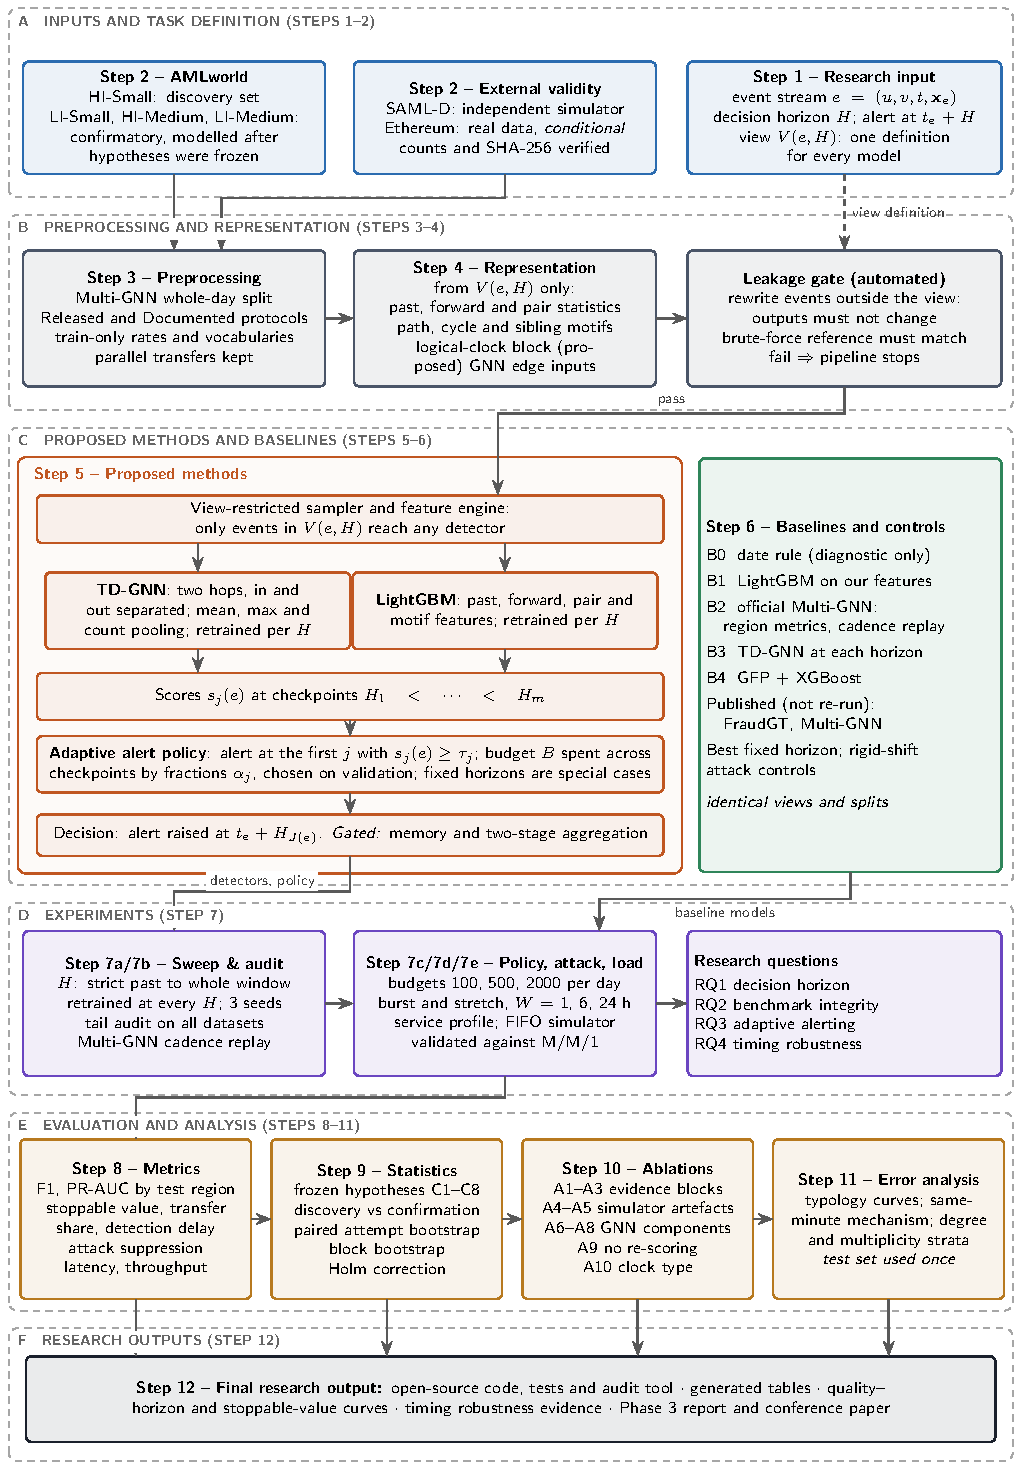
\includegraphics[width=0.98\textwidth,height=0.78\textheight,keepaspectratio]{methodology_architecture.pdf}
    \caption{Research methodology architecture of the decision-horizon study. The twelve steps are organised in six bands: (A) inputs and task definition (Steps 1--2), (B) preprocessing and representation (Steps 3--4), (C) proposed methods and baselines (Steps 5--6), (D) experiments (Step 7), (E) evaluation and analysis (Steps 8--11), and (F) research outputs (Step 12). Dashed arrows denote the view definition and the frozen hypotheses, which constrain later stages without passing data.}
    \label{fig:methodology_architecture}
\end{figure}

\subsection{Architectural Narrative and Operational Band Dynamics}
\begin{enumerate}[leftmargin=*]
    \item \textbf{Band A (Steps 1--2):} AMLworld (discovery and confirmatory datasets), SAML-D and, conditionally, Ethereum enter as verified event streams. The view $V(e,H)$ is defined once here.
    \item \textbf{Band B (Steps 3--4):} the Multi-GNN split under the Released and Documented protocols, followed by horizon-aware features. The automated gate stops the pipeline if rewriting events outside the view changes any output.
    \item \textbf{Band C (Steps 5--6):} per-horizon detectors (LightGBM and TD-GNN) feed the adaptive alert policy. The official Multi-GNN, GFP, the date rule and published values are the comparators.
    \item \textbf{Band D (Step 7):} the horizon sweep, the benchmark audit with cadence replay, adaptive alerting, the timing-only attack with matched controls on wall-clock and logical-clock detectors, and service times with queue simulation, mapped to RQ1--RQ4.
    \item \textbf{Band E (Steps 8--11):} metrics by test region, including stoppable value; discovery versus confirmation against frozen hypotheses; ablations that include simulator-artefact checks and the price of timing robustness; per-typology error analysis.
    \item \textbf{Band F (Step 12):} code, audit tool, generated tables, the Phase 3 report and a conference paper.
\end{enumerate}

% =========================================================================
% Project Execution Plan, Feasibility, and Risk Management
% =========================================================================
\section{Project Execution Plan, Feasibility, and Risk Management}
\label{sec:execution_plan}

\subsection{Milestones}
The instructor has confirmed that 15 November 2026 is a progress milestone, not the final deadline. The plan aims for credible evidence by that date, with the publication standard as the target beyond it. Table~\ref{tab:phase3_plan} lists the milestones; the detailed schedule is kept in \texttt{ROADMAP.md}.

\begin{table}[htbp]
\centering
\scriptsize
\caption{Milestones and Decision Gates (2026--2027). Dates after 15 November are planning targets; venue dates are in Section~\ref{sec:publication_potential}.}
\label{tab:phase3_plan}
\begin{tabularx}{\textwidth}{L{0.8cm} L{1.5cm} X L{2.3cm} L{3.2cm}}
\toprule
\textbf{ID} & \textbf{Dates} & \textbf{Work} & \textbf{Where} & \textbf{Exit criterion} \\
\midrule
M0 & 1 Nov & HI-Small discovery: audit, main horizon sweep; hypotheses frozen & Done & Section~\ref{sec:preliminary} \\
\midrule
M1 & 2--4 Nov & Move code to a shared repository; run the leakage checks at all horizons & Kaggle CPU & All shuffled-label runs collapse to prevalence \\
\midrule
M2 & 2--7 Nov & Official Multi-GNN: stock run, region metrics, cadence replay; GFP & Kaggle GPU (Multi-GNN), Kaggle CPU (GFP) & Published HI-Small F1 reproduced within its spread, or documented as not reproduced \\
\midrule
G1 & 7 Nov & Does the official GNN show the tail and horizon effects? & --- & Decides whether the claim covers GNNs or only our models \\
\midrule
M3 & 3--10 Nov & Confirmatory sweeps; alert policy; TD-GNN at several horizons & molab or Kaggle CPU; MacBook (Medium); Kaggle or university GPU (TD-GNN) & Verdict for each frozen hypothesis \\
\midrule
M4 & 5--12 Nov & Timing attack; logical-clock detector; ablations; service profile & Kaggle CPU; university GPU (latency) & Attack table with controls; price of robustness \\
\midrule
\textbf{P} & \textbf{15 Nov} & \textbf{Progress milestone:} report covering all seven brief components, each marked complete or preliminary & --- & Submitted \\
\midrule
G2 & late Nov & Is there a modelling gap at small horizons worth closing with memory or two-stage aggregation? & --- & Build DMT-GNN only if yes \\
\midrule
M5 & Dec & Rolling-origin folds; per-attempt attacks; real Ethereum window; search repeated; maintainers contacted & All & Results robust across folds \\
\midrule
M6 & Jan--Feb 2027 & Paper draft and artefact release & All & Submission if the venue's call opens \\
\bottomrule
\end{tabularx}
\end{table}

\subsection{Compute Strategy}
\label{sec:compute_strategy}
\paragraph{Principle.} No single machine is a dependency. Every job is a script that takes a dataset and writes a results folder, so it can run wherever capacity exists. Team laptops are for development and analysis.

\paragraph{Resources and allocation.} Table~\ref{tab:compute_budget} assigns each experiment to a resource. Only the official Multi-GNN strictly needs a GPU; TD-GNN benefits from one. Measured figures come from the discovery runs on an Intel i5-1235U, where a LightGBM run took about one to two minutes on HI-Small, including features. All other figures are planning estimates until measured. Kaggle's quota is commonly reported as about 30 GPU hours per week per account, which is unofficial and must be confirmed in the team's accounts. A friend's GPU is treated as extra capacity until its specification is known.

\begin{table}[htbp]
\centering
\scriptsize
\caption{Compute Plan by Experiment. GPU hours are estimates except where marked; the only published anchor is about 3.6\,h for one Multi-GNN run on an RTX 3090 \cite{egressy2024multigraph}.}
\label{tab:compute_budget}
\begin{tabularx}{\textwidth}{L{4.2cm} L{3.6cm} L{1.6cm} X}
\toprule
\textbf{Experiment} & \textbf{Where} & \textbf{GPU hours} & \textbf{Notes} \\
\midrule
Official Multi-GNN: GIN, PNA, second seed & Kaggle GPU; university GPU as fallback & 12--24 & 4--8\,h per run assumed; cadence replay included; harness not yet executed \\
TD-GNN: 4 horizons $\times$ 3 seeds & Kaggle or university GPU; Colab overflow & 12--24 & Unmeasured: no full run has finished \\
TGN comparison, if gate G2 passes & Kaggle GPU & 10--20 & Gated \\
Service and GPU latency profile & University GPU & 2--3 & Needs one consistent device \\
LightGBM on LI-Small, attacks, ablations, leakage checks & Kaggle CPU or molab (32\,GB) & 0 & About one to two minutes per run at HI-Small scale \\
LightGBM on HI-Medium, LI-Medium & MacBook (32\,GB) or molab & 0 & About six times larger; \texttt{prepare.py} needs memory work first \\
GFP & Kaggle CPU (Linux) & 0 & Library is not supported on Windows \\
\midrule
\textbf{Total} & & \textbf{26--51} & \textbf{Plus 10--20 if gated work runs} \\
\bottomrule
\end{tabularx}
\end{table}

\paragraph{Hosted notebooks: molab.} molab, the hosted notebook service of the marimo project, provides free notebooks with 4 CPUs and 32\,GB of RAM and, as a public preview, an optional NVIDIA RTX Pro 6000 Blackwell GPU with 96\,GB of memory; a notebook runs for at most 12\,h and is shut down after more than 90 minutes of inactivity.\footnote{\url{https://docs.marimo.io/guides/molab/}, accessed 25 October 2026.} Its large memory makes it useful for the Medium datasets. We rely on it only after three acceptance tests (GPU attachment, survival of a two-hour job with the browser closed, and data-loading time). Notebooks are public by default, so no credentials may appear in notebook code.

\subsection{Risk Assessment and Mitigation Strategies}
Table~\ref{tab:risk_management} lists the main technical and scientific risks.

\begin{table}[htbp]
\centering
\small
\caption{Risk Assessment and Mitigation Strategy Matrix}
\label{tab:risk_management}
\begin{tabularx}{\textwidth}{L{2.7cm} L{3.4cm} L{1.2cm} X}
\toprule
\textbf{Identified Risk} & \textbf{Operational Impact} & \textbf{Level} & \textbf{Mitigation Strategy} \\
\midrule
\textbf{R1: Effects are feature-model specific} & The official GNN may not show the same dependence on look-ahead or tail. & High & M2 tests this directly on the official code, and gate G1 reports it either way. A narrower claim is still a valid finding. \\
\midrule
\textbf{R2: Simulator artefact} & Same-minute bursts and timing may reflect AMLworld's scheduler, not laundering. & High & SAML-D as an independent simulator; hour and format ablations; real Ethereum window. No real-world effect sizes are claimed. \\
\midrule
\textbf{R3: Scooped} & The audit or a timing attack appears first; Heijmans et al.\ (October 2026) name timestamps as future work. & Medium & Search repeated monthly and before submission; move quickly on the audit; consider a preprint. \\
\midrule
\textbf{R4: Too few attempts} & 86 test attempts on HI-Small give wide attempt-level intervals. & High & HI-Medium; rolling-origin folds; attempt-level bootstrap reported honestly. \\
\midrule
\textbf{R5: Logical-clock defence costs too much} & Robust evidence may lose too much clean-data quality, since wall-clock gaps carry real signal. & High & This is a measured outcome (A10). A combined detector is also tested; a negative result is reported. \\
\midrule
\textbf{R6: Our GNN underperforms} & TD-GNN is weak, so its horizon curve says little about GNNs. & Medium & The official Multi-GNN is the reference; TD-GNN results are reported relative to it. \\
\midrule
\textbf{R7: Metric criticism} & Stoppable value assumes alerts can stop later transfers and can double count funds across hops. & Medium & Stated plainly; transfer-count analogue always reported; hop-aware variant planned. \\
\midrule
\textbf{R8: Multi-GNN audit fails to run} & The harness has never been executed, and the official code may not run on current libraries. & Medium & Pinned environment on Kaggle; a time box; otherwise published values are labelled as not reproduced. \\
\midrule
\textbf{R9: Leakage bugs} & Inflated horizon results. & Moderate & Future-perturbation tests, brute-force reference and mutation checks; shuffled-label runs at every horizon (M1). \\
\midrule
\textbf{R10: Compute access} & Quotas or access are lower than assumed. & Moderate & Several interchangeable resources; every job is resumable by re-running one script. \\
\midrule
\textbf{R11: Responsible disclosure and ethics} & Findings could be misread as an attack on a named benchmark or as evasion guidance. & Low & Synthetic data only; defences reported with the attack; dataset maintainers contacted before publication. \\
\bottomrule
\end{tabularx}
\end{table}

% =========================================================================
% Publication Potential
% =========================================================================
\section{Preliminary Evidence (1 November 2026)}
\label{sec:preliminary}
Every number in this section is generated from experiment logs by a script; tables and in-text values are not typed by hand. These are \textbf{discovery results on HI-Small}, except the day-level counts in Section~\ref{sec:prelim_tail}, which cover all four datasets. They use our own detector. \textbf{The official Multi-GNN has not been run}, so statements about published models remain inferences from their code.

\subsection{What Has and Has Not Been Run}
\begin{table}[htbp]
\centering
\small
\caption{Status of Experiments}
\label{tab:prelim_status}
\begin{tabularx}{\textwidth}{L{5.4cm} L{2.2cm} X}
\toprule
\textbf{Experiment} & \textbf{Status} & \textbf{Note} \\
\midrule
Tail audit, four datasets & Complete & Day-level counts only; no modelling \\
Horizon sweep, HI-Small, Released protocol & Complete & 9 horizons, 3 seeds \\
Horizon sweep, HI-Small, Documented protocol & Partial & Complete to 1\,h; run stopped \\
Shuffled-label leakage check & Partial & \SanityHorizonsDone{} of 4 horizons \\
Adaptive alert policy & Partial & One seed \\
Feature and GNN ablations & Not run & \\
Timing attack & Not run & Code written and tested \\
TD-GNN & Not run & Code written and tested; no full run finished \\
Official Multi-GNN audit & Not run & Harness written but never executed \\
GFP; SAML-D; LI-Small and Medium models & Not run & Reserved for confirmation \\
Logical-clock detector & Not built & Proposed \\
\bottomrule
\end{tabularx}
\end{table}

\paragraph{Verification.} All 119 automated tests pass. They include a brute-force reference for the feature engine, tests that rewrite data outside the view and require unchanged output, attack invariants, and a queue simulator check against the M/M/1 closed form. The strict-past results are identical with and without the tail days in the file, as causality requires. With shuffled training labels at strict past, core PR-AUC is \SanityShuffledStrict{}, against a prevalence of \SanityPrev{}, so the model finds nothing. \emph{This check has not yet been completed at positive horizons, where leakage matters most; until it is, positive-horizon results carry that caveat.}

\subsection{The Benchmark Tail}
\label{sec:prelim_tail}
Table~\ref{tab:tail} and Figure~\ref{fig:tail} report the day-level audit. On every dataset, background traffic stops at the span documented by Altman et al.\ \cite{altman2023ibmaml}, and laundering continues. The Multi-GNN split places those days in the test set. On HI-Small, \TailHISmallEvents{} events (\TailHISmallRate\% illicit) hold \TailHISmallShare\% of the test set's illicit transfers.

\begin{table}[htbp]
\centering
\caption{The post-simulation tail on AMLworld. The date rule flags every transfer in the tail. \emph{It is a diagnostic, not a detector}: it has no learning, and it uses knowledge of the tail. Published values are from Egressy et al.\ \cite{egressy2024multigraph}, not re-run.}
\label{tab:tail}
\resizebox{\textwidth}{!}{\begin{tabular}{lrrrrrrrr}
\toprule
Dataset & Days in file & Documented & Tail events & Tail illicit & Share of test & Date-rule & XGB+GFs & Multi-PNA+EU \\
 & & days & & rate (\%) & illicit (\%) & F1 (\%) & (publ.) & (publ.) \\
\midrule
HI-Small & 18 & 10 & 1,108 & 59.1 & 40.7 & 48.18 & 63.23 & 68.16 \\
LI-Small & 17 & 10 & 223 & 60.1 & 16.7 & 26.15 & 27.30 & 33.07 \\
HI-Medium & 28 & 16 & 6,987 & 58.5 & 37.1 & 45.37 & 65.70 & 65.67 \\
LI-Medium & 27 & 16 & 1,370 & 56.3 & 19.3 & 28.76 & 28.16 & 33.23 \\
\bottomrule
\end{tabular}}
\end{table}

\begin{figure}[htbp]
\centering
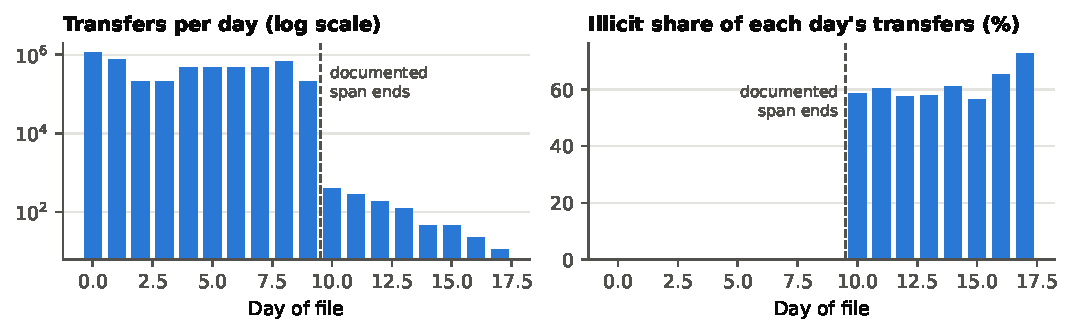
\includegraphics[width=\textwidth]{generated/fig_tail.pdf}
\caption{HI-Small by day. After the documented 10-day span, daily volume falls by about three orders of magnitude, while the illicit share rises to about 60\%. Most of the test split's days lie in this region.}
\label{fig:tail}
\end{figure}

The date rule scores \TailHISmallFone\% F1 on HI-Small, above the 47.73\% published for GIN+EU, and \TailLIMediumFone\% on LI-Medium, above the 28.16\% published for XGBoost with graph features. This does not show that those models exploit the tail. It shows that the metric's value is sensitive to a region that contains almost no negatives. How much of each published number comes from there is what the Multi-GNN audit will measure.

\subsection{Quality Against Horizon}
Table~\ref{tab:horizon} and Figure~\ref{fig:horizon} give the sweep on the discovery set, with LightGBM retrained at every horizon.

\begin{table}[htbp]
\centering
\small
\caption{Horizon sweep, HI-Small, Released protocol (LightGBM, mean over 3 seeds, $\pm$ s.d.). SV$_B$ is mean stoppable value at $B$ alerts/day with thresholds set on validation. Detection is at $B=500$. ``Core'' removes the tail. Attempts: \HISAttempts{}.}
\label{tab:horizon}
\resizebox{\textwidth}{!}{\begin{tabular}{lrrrrrrr}
\toprule
Horizon $H$ & Test F1 & Core F1 & Core PR-AUC & Detected & SV$_{100}$ & SV$_{500}$ & SV$_{2000}$ \\
\midrule
strict past & 54.4$\pm$0.5 & 37.7$\pm$0.1 & 0.364 & 93\% & 0.287 & 0.578 & 0.629 \\
same minute & 66.7$\pm$0.4 & 52.3$\pm$0.7 & 0.521 & 97\% & 0.319 & 0.617 & 0.634 \\
1 min & 66.6$\pm$1.2 & 52.5$\pm$1.6 & 0.526 & 96\% & 0.310 & 0.617 & 0.638 \\
10 min & 70.3$\pm$0.8 & 57.0$\pm$0.9 & 0.546 & 98\% & 0.281 & 0.611 & 0.635 \\
1 h & 73.5$\pm$0.3 & 62.7$\pm$0.6 & 0.575 & 95\% & 0.301 & 0.611 & 0.623 \\
6 h & 72.7$\pm$0.2 & 61.4$\pm$0.9 & 0.574 & 96\% & 0.276 & 0.570 & 0.589 \\
24 h & 72.9$\pm$1.1 & 61.5$\pm$0.5 & 0.572 & 94\% & 0.177 & 0.438 & 0.457 \\
72 h & 72.0$\pm$1.1 & 60.9$\pm$0.5 & 0.576 & 95\% & 0.070 & 0.180 & 0.185 \\
whole window & 71.9$\pm$0.3 & 61.0$\pm$0.4 & 0.563 & 94\% & 0.000 & 0.000 & 0.000 \\
\bottomrule
\end{tabular}}
\end{table}

\begin{figure}[htbp]
\centering
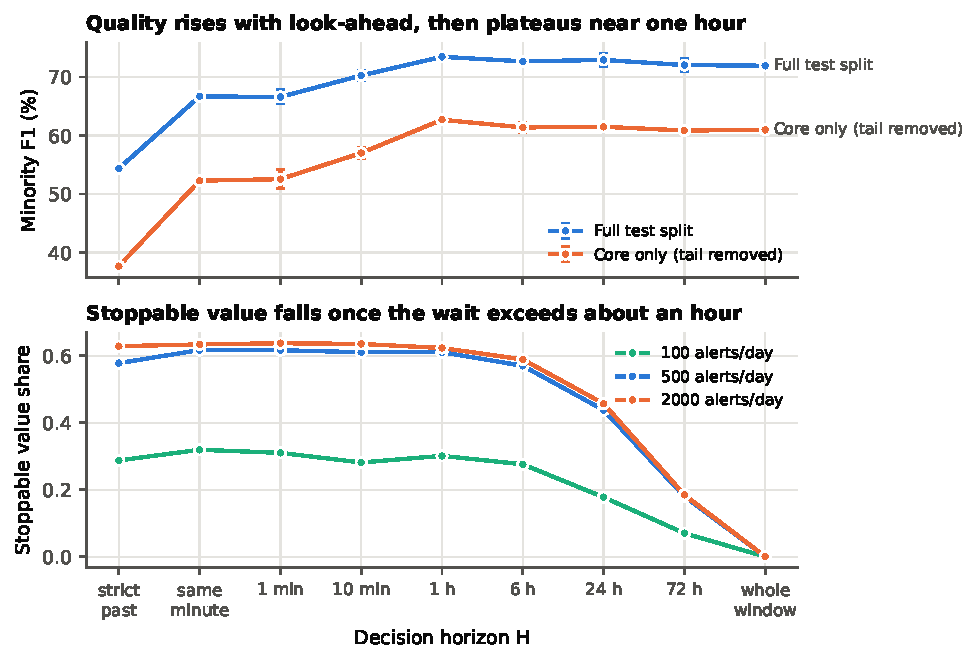
\includegraphics[width=0.86\textwidth]{generated/fig_horizon.pdf}
\caption{Quality and stoppable value against decision horizon, HI-Small, Released protocol. The two panels use separate axes because the measures differ in scale. Error bars show one s.d.\ over seeds. Table~\ref{tab:horizon} gives the values.}
\label{fig:horizon}
\end{figure}

Four observations follow, each limited to this dataset and detector:
\begin{enumerate}[leftmargin=*]
    \item \textbf{Look-ahead has a large effect.} Test F1 rises from \HISFStrict\% (strict past) to \HISFHour\% (1\,h). On the core alone, it rises from \HISCoreFStrict\% to \HISCoreFHour\%, and PR-AUC from \HISCorePRStrict{} to \HISCorePRHour.
    \item \textbf{The gain plateaus near one hour.} From 1\,h to the whole window, core PR-AUC changes by \HourToInfPR. The published protocol's multi-day view may add little for this detector, compared with a far shorter wait.
    \item \textbf{The tail raises F1.} At the whole-window view, test F1 is \COneGap{} points above core F1.
    \item \textbf{Real-time performance is an interval.} The strict-past and same-minute views differ in core PR-AUC by \CFourGap. Same-minute events have unknown order, and they matter: \SameMinInflowIllicit\% of illicit core transfers have a sender receiving funds in the same minute, against \SameMinInflowBenign\% of benign ones. Funds must arrive before they are forwarded, so a real system with sub-minute ordering could see part of this. Whether this reflects laundering or the simulator's scheduler is an open question that SAML-D will help answer.
\end{enumerate}
As a check on the baseline, our same-minute view (\HISFTie\% test F1) is at or above GFP's published 63.23\% at batch size 128, so the causal baseline is not artificially weak. These values are not directly comparable with published GNN results: the features, thresholding and training differ.

\subsection{F1 and Stoppable Value Disagree}
F1 changes little from 1\,h to 24\,h, while stoppable value at 500 alerts/day falls from \HISSVHour{} to \HISSVDay. The paired contrast between the best horizon of at most 1\,h and 24\,h is \HISCThreeValDiff{} (95\% CI \HISCThreeValCI). By construction, value reaches zero at the whole window, where F1 remains high: on this measure, a whole-window evaluation describes a detector that acts only after the attempts it detects have finished.

\begin{table}[htbp]
\centering
\small
\caption{Stoppable value at 500 alerts/day under two threshold rules, HI-Small, Released protocol. ``Val.'' sets thresholds on validation, as a deployment would. ``Equal alerts'' gives every horizon the same alert count on the test window, as a sensitivity analysis. ``Transfers'' is the transfer-count analogue of SV.}
\label{tab:sv}
\resizebox{\textwidth}{!}{\begin{tabular}{lrrrr}
\toprule
Horizon $H$ & SV$_{500}$ (val.\ threshold) & Transfers (val.) & SV$_{500}$ (equal alerts) & Detected (equal alerts) \\
\midrule
strict past & 0.578 & 0.578 & 0.428 & 74\% \\
same minute & 0.617 & 0.623 & 0.557 & 89\% \\
1 min & 0.617 & 0.620 & 0.573 & 92\% \\
10 min & 0.611 & 0.617 & 0.576 & 93\% \\
1 h & 0.611 & 0.617 & 0.571 & 90\% \\
6 h & 0.570 & 0.569 & 0.531 & 90\% \\
24 h & 0.438 & 0.437 & 0.411 & 88\% \\
72 h & 0.180 & 0.175 & 0.152 & 87\% \\
whole window & 0.000 & 0.000 & 0.000 & 85\% \\
\bottomrule
\end{tabular}}
\end{table}

\paragraph{A bias we corrected.} Thresholds set on validation do not produce equal alert rates on test: at a nominal 500 alerts/day, the strict-past detector actually raises \AlertsStrict{} alerts per day in the core and the 1\,h detector \AlertsHour. This favours strict past. With alerts equalised (Table~\ref{tab:sv}), waiting is clearly better: the gain of the best short horizon (\HISCThreeTestBest) over strict past is \HISWaitGainTest{} (95\% CI \HISWaitGainTestCI). \textbf{The practical reading on this dataset is to wait a little, not long.} A short wait gains evidence while most of an attempt's funds have yet to move, because attempts unfold over days. This depends on the simulator's timing: real laundering that moves faster would shorten the useful wait, which is why the result needs independent data.

\paragraph{Documented protocol.} Removing the tail truncates attempts at the end of the window, so stoppable value is lower throughout (Table~\ref{tab:sv_documented}), but the shape from strict past to 1\,h is the same.

\begin{table}[htbp]
\centering
\small
\caption{Stoppable value at 500 alerts/day, HI-Small, Documented protocol. Only horizons with all three seeds complete are shown; the run was stopped before 6\,h.}
\label{tab:sv_documented}
\resizebox{\textwidth}{!}{\begin{tabular}{lrrrr}
\toprule
Horizon $H$ & SV$_{500}$ (val.\ threshold) & Transfers (val.) & SV$_{500}$ (equal alerts) & Detected (equal alerts) \\
\midrule
strict past & 0.286 & 0.307 & 0.236 & 73\% \\
same minute & 0.355 & 0.370 & 0.339 & 90\% \\
1 min & 0.351 & 0.366 & 0.337 & 89\% \\
10 min & 0.354 & 0.369 & 0.347 & 92\% \\
1 h & 0.341 & 0.357 & 0.341 & 90\% \\
\bottomrule
\end{tabular}}
\end{table}

\paragraph{By typology.} Table~\ref{tab:typology} shows that the pattern holds across most typologies, though with few attempts per typology. Bipartite attempts yield the least stoppable value at every horizon shown.

\begin{table}[htbp]
\centering
\small
\caption{Detection and stoppable value by typology at 500 alerts/day, HI-Small. Each typology has few attempts, so differences between typologies are indicative only.}
\label{tab:typology}
\resizebox{0.82\textwidth}{!}{\begin{tabular}{lrrrrrrrrr}
\toprule
Typology & $n$ & \multicolumn{2}{c}{strict past} & \multicolumn{2}{c}{same minute} & \multicolumn{2}{c}{1 h} & \multicolumn{2}{c}{24 h} \\
 & & Det. & SV & Det. & SV & Det. & SV & Det. & SV \\
\midrule
Bipartite & 15 & 80\% & 0.19 & 87\% & 0.22 & 82\% & 0.21 & 80\% & 0.10 \\
Cycle & 9 & 100\% & 0.73 & 100\% & 0.77 & 100\% & 0.78 & 100\% & 0.48 \\
Fan-In & 9 & 93\% & 0.68 & 100\% & 0.70 & 89\% & 0.70 & 100\% & 0.53 \\
Fan-Out & 9 & 89\% & 0.66 & 89\% & 0.67 & 89\% & 0.67 & 93\% & 0.51 \\
Gather-Scatter & 16 & 98\% & 0.87 & 100\% & 0.85 & 100\% & 0.85 & 100\% & 0.68 \\
Random & 12 & 92\% & 0.41 & 100\% & 0.52 & 100\% & 0.52 & 97\% & 0.41 \\
Scatter-Gather & 10 & 100\% & 0.70 & 100\% & 0.73 & 100\% & 0.68 & 100\% & 0.52 \\
Stack & 6 & 94\% & 0.39 & 100\% & 0.55 & 100\% & 0.58 & 83\% & 0.24 \\
\bottomrule
\end{tabular}}
\end{table}

\subsection{Adaptive Alerting: Incomplete}
Table~\ref{tab:policy_partial} shows the only completed policy run, one seed of three. Adaptive allocation beats the best fixed horizon at 100 alerts/day, where the budget binds hardest; at higher budgets the interval includes zero. One seed cannot settle this, but it tempers expectations: one good fixed horizon may suffice.

\begin{table}[htbp]
\centering
\small
\caption{Adaptive alert policy against the best fixed horizon selected on validation, HI-Small, Released protocol. \emph{One seed only; the run was stopped.}}
\label{tab:policy_partial}
\begin{tabular}{rrrrl}
\toprule
Budget & Adaptive SV & Best fixed SV & Difference & 95\% CI \\
\midrule
100 & 0.305 & 0.273 & +0.031 & [+0.008, +0.059] \\
500 & 0.623 & 0.615 & +0.008 & [-0.004, +0.025] \\
2000 & 0.640 & 0.636 & +0.004 & [-0.002, +0.014] \\
\bottomrule
\end{tabular}
\end{table}

\subsection{Hypothesis Status}
Hypotheses were frozen in \texttt{DECISIONS.md} before any model ran on the confirmatory datasets. \textbf{None has yet been tested on confirmatory data.} HI-Small cannot confirm them, because it suggested them.

\begin{table}[htbp]
\centering
\small
\caption{Frozen Hypotheses and Current Evidence}
\label{tab:hypotheses}
\begin{tabularx}{\textwidth}{L{0.7cm} X L{4.3cm} L{1.9cm}}
\toprule
\textbf{ID} & \textbf{Claim} & \textbf{Discovery set (HI-Small)} & \textbf{Confirmation} \\
\midrule
C1 & The tail inflates headline F1 by more than 5 points & \COneGap{} points & Pending \\
C2 & Look-ahead is worth more than 0.05 core PR-AUC & \CTwoGap & Pending \\
C3 & F1 and stoppable value disagree on the best horizon & \HISCThreeValDiff{}, CI \HISCThreeValCI & Pending \\
C4 & Real-time performance is an interval wider than 0.02 PR-AUC & \CFourGap & Pending \\
C5 & Adaptive alerting beats the best fixed horizon at $B=500$ & One seed; CI includes zero & Pending \\
C6 & Bursts evade strict-past detectors; same-minute visibility blunts this & Not run & Pending \\
C7 & Equal views change the GNN versus boosted-tree comparison & Not run & Pending \\
C8 & Logical-clock evidence resists stretch attacks at acceptable clean-data cost & Not built & Pending \\
\bottomrule
\end{tabularx}
\end{table}

\section{Publication Potential}
\label{sec:publication_potential}

\subsection{Novelty and Scientific Contribution Assessment}
Publication is plausible but not assured. We assess each part as a sceptical reviewer would, in descending order of current confidence:
\begin{enumerate}[leftmargin=*]
    \item \textbf{Benchmark audit (strong).} The tail is verifiable by anyone from the public files, and it affects a benchmark that recent work ranks models on. Daniluk and Dabrowski's finding on TGB \cite{daniluk2023global} shows that such results are publishable. Its effect on specific published numbers still has to be shown on their code.
    \item \textbf{Horizon curves and the F1--value conflict (promising).} This changes what readers should ask of a detector. Nguyen et al.\ \cite{nguyen2022future} already show that the future helps in card fraud, so our contribution is the graph setting, the cost side of the trade-off, and equal-view comparisons. It rests so far on one dataset and one model family.
    \item \textbf{Timing-only threat model (open but time-sensitive).} We found no prior timing-only attack on these models, but we have run no attack yet, and recent work names it as an extension \cite{heijmans2026robust}.
    \item \textbf{Timing-invariant detection (highest potential, least evidence).} This is the most original idea here and has real-world appeal: robustness by design, without attack examples or adversarial training. It is an untested hypothesis, and it may cost too much clean-data quality.
    \item \textbf{Adaptive alerting (weak so far).} In one incomplete seed, it barely beats one good fixed horizon except at the smallest budget. If this holds, the honest and useful conclusion is that one simple short wait suffices.
    \item \textbf{Modelling (deliberately de-emphasised).} DMT-GNN is incremental next to MEGA-GNN, DIAM and SALT-GNN \cite{bilgi2026mega,ding2024diam,losavio2026saltgnn}.
\end{enumerate}

\paragraph{Real-world impact.} If confirmed, the findings would give three concrete pieces of guidance: report the decision horizon alongside any AML result; evaluate alerts by what they can still stop, not only by F1; and prefer evidence an adversary cannot change by re-timing. The first two need no new model and could be adopted immediately. All of this is on synthetic data so far, and it does not establish effect sizes in a real institution.

\paragraph{Minimum evidence for a credible submission.} (i) The official Multi-GNN audited by region and view; (ii) horizon curves for at least two model families on at least two simulators; (iii) confirmed hypotheses on data unseen at freezing; (iv) robustness across rolling-origin folds; (v) released code and audit tool; and (vi) a repeated literature search.

\subsection{Target Publication Venues}
Two papers are more defensible than one overloaded paper: \textbf{Paper A} (benchmark audit, horizon framework, stoppable value) and \textbf{Paper B} (timing-only threat model and timing-invariant detection). Facts below were checked on official pages on 1 November 2026, except where marked. Rankings are not re-verified here and should be confirmed on the ICORE portal.
\begin{itemize}[leftmargin=*]
    \item \textbf{Paper A, primary: KDD 2027, Datasets and Benchmarks track} (San Jose, 1--5 August 2027). Its scope explicitly includes benchmarks, evaluation methods and auditing frameworks, with eight content pages, single-blind review and at least three reviews. Cycle 1 closed on 26 July 2026. The Research Track's page refers to a February 2027 deadline; \emph{a second-cycle call for this track was not yet published} when checked, so this date must be confirmed.
    \item \textbf{Paper A, alternative: ACM ICAIF 2027.} GFP, FraudGT and LAS-GNN appeared there \cite{blanusa2024gfp,lin2024fraudgt,verlaan2025lasgnn}, so its reviewers know this benchmark. ICAIF 2026 had an August deadline, an eight-page limit including references, double-blind review and no appendices. \emph{The 2027 call was not yet published; an August 2027 deadline is an inference.}
    \item \textbf{Paper B: Financial Cryptography and Data Security (FC).} FC 2027 closed on 17 September 2026 (Barbados, February 2027), with regular papers of 15 pages plus references in LNCS format, anonymised. FC 2028 is the realistic target, and only if the attack holds beyond one simulator. \emph{Its dates are not published.}
    \item \textbf{Alternatives:} ECML PKDD 2027 Applied Data Science (the 2026 deadline was 12 March; 2027 dates unconfirmed); the Learning on Graphs conference (2026 deadline in August; nine-page proceedings track); the Temporal Graph Learning workshop, where Daniluk and Dabrowski appeared (2027 edition unconfirmed).
    \item \textbf{Not recommended now:} main research tracks of top ML venues, which expect a new method with a large effect on multiple real datasets, and networking flagships, where the systems component is too small to carry a paper on its own. Deadlines for IEEE ICC, GLOBECOM, ICBC and ACM AFT could not be confirmed from official pages and were not assessed.
\end{itemize}
Before any submission, the literature search of Section~\ref{sec:selection} is repeated, the benchmark's maintainers are contacted, and the Official Journal text of Regulation 2024/886 is checked directly.

% =========================================================================
% Conclusion
% =========================================================================
\section{Conclusion}
\label{sec:conclusion}

This document extends the Phase 1 review with nine verified 2025--2026 studies from Q1/Q2 journals and CORE A* conferences, positions the project against the closest earlier work, and turns the resulting gaps into a twelve-step methodology.

Revision 3 changes the direction of the project on the basis of direct evidence. Reading the released code shows that the most-cited AML results use an unstated, non-uniform view of future transactions. Reading the raw data shows that the standard test split extends past the end of background traffic on all four datasets we checked. Preliminary measurements on the discovery set suggest that strict causality costs a large share of detection quality, that the gain from looking ahead plateaus near an hour for our feature-based detector, and that F1 and stoppable value disagree about how long to wait: a short wait pays, a long one does not. These are discovery results on one dataset and one family of models. The official GNN has not yet been run, and the hypotheses that would make these results general are frozen and untested.

The Computer Networks contribution lies in treating detection as a delay--information trade-off in a stream-processing service, and in proposing logical rather than physical time as the basis for evidence an adversary cannot move. The project's aim remains a defensible conference paper; 15 November 2026 is the first evidence-of-progress milestone on the way.

% =========================================================================
% Appendices
% =========================================================================
\appendix

\section{Requirement Traceability Matrix}
\label{app:traceability}

Table~\ref{tab:traceability_matrix} maps each Phase 2 requirement to where it is addressed.

\begin{table}[htbp]
\centering
\scriptsize
\caption{Phase 2 Requirement Traceability Matrix}
\label{tab:traceability_matrix}
\begin{tabularx}{\textwidth}{L{4.6cm} X L{3.6cm}}
\toprule
\textbf{Requirement} & \textbf{How it is addressed} & \textbf{Location} \\
\midrule
8--10 additional papers, 2025--2026 & Nine papers; Phase 1 papers excluded; years verified on Crossref & Section~\ref{sec:selection}, Table~\ref{tab:eligibility_audit} \\
Genuine research articles in Q1/Q2 or ranked venues & Seven journal articles (Q1/Q2) and two CORE A* conference papers; sources in Appendix~\ref{app:verification} & Table~\ref{tab:eligibility_audit} \\
Relevance, methodology, data and evaluation & Fifteen headings (A--O) per paper & Section~\ref{sec:individual_analyses} \\
Screening transparency & Excluded candidates with reasons & Table~\ref{tab:excluded} \\
Cross-paper comparison table (title, year, dataset, preprocessing, models, metrics, results, limitations) & Landscape table with split protocol stated; capability matrix & Tables~\ref{tab:cross_paper_comparison}, \ref{tab:capability_matrix} \\
At least three research gaps with evidence from three papers & Six gaps (G4 deferred; G5 and G6 added in Revision 3), evidence from KAR, LMAE4Eth, TAML and the code audits & Table~\ref{tab:gap_synthesis}, Section~\ref{sec:gap_justification} \\
Refined gap answering six questions & Six questions; gap statement, problem, aim, objectives, RQ1--RQ4 & Section~\ref{sec:refined_gap} \\
Twelve-step methodology & Steps 1--12 with objective, input, procedure, output, justification, literature, risks & Section~\ref{sec:methodology}, Table~\ref{tab:methodology_summary} \\
Methodology architecture diagram & Vector TikZ figure consistent with Steps 1--12 & Figure~\ref{fig:methodology_architecture} \\
Feasibility within the project timeline & Revision 3: milestones and gates to the 15 November progress date and beyond; CPU-first compute strategy; risks & Section~\ref{sec:execution_plan}, Tables~\ref{tab:phase3_plan}, \ref{tab:risk_management} \\
Publication potential & Contribution assessment and venue fit & Section~\ref{sec:publication_potential} \\
Closest prior work & Multi-GNN, DIAM, MEGA-GNN, GFP, FraudGT (with reported results), SALT-GNN, PRES, BADGNN, AnchorRM, StreamTGN, TeMP-TraG, Amatriciana; added in Revision 3: KONTOGRAPH, Maganti, MemFreezing, HIA, TDAP, Heijmans et al., LAS-GNN & Section~\ref{sec:prior_work}, Table~\ref{tab:prior_work_positioning} \\
\bottomrule
\end{tabularx}
\end{table}

\section{Literature Verification Log}
\label{app:verification}

Bibliographic metadata were checked against Crossref (\texttt{api.crossref.org}) and the publisher landing pages in October 2026. Conference ranks were checked on the ICORE portal. The SCImago portal blocked automated access, so journal quartiles come from publisher bibliometric pages or secondary SJR/JCR listings and should be re-confirmed on \url{https://www.scimagojr.com} before final submission. The entries added in Revision 2 (below the FraudGT row) come from arXiv abstract pages and, for StreamTGN, search-result excerpts; at that time their full texts were still to be read, and none of them is counted towards the nine-paper quota. On 1 November 2026, the full texts of AnchorRM, StreamTGN, MemFreezing, HIA, KONTOGRAPH, Maganti and Heijmans et al.\ and the relevant sections of Multi-GNN, MEGA-GNN, GFP and SALT-GNN were read; the Multi-GNN repository (commit \texttt{252b025}) and FraudGT's dataset class were inspected directly. LAS-GNN and TDAP were checked against Crossref metadata only; LAS-GNN's full text was not accessible. Regulation 2024/886 was cited from secondary sources because EUR-Lex could not be read automatically. Searches that found no prior work on the AMLworld tail, on horizon curves or on timing-only attacks do not prove none exists.

\begin{table}[htbp]
\centering
\scriptsize
\caption{Literature Verification Log}
\label{tab:verification_log}
\begin{tabularx}{\textwidth}{L{1.7cm} L{2.9cm} L{2.6cm} L{2.3cm} X}
\toprule
\textbf{Key} & \textbf{First author, year, venue} & \textbf{DOI / identifier} & \textbf{Ranking (source)} & \textbf{Full text examined; notes} \\
\midrule
\texttt{yang2025} & X.~Yang, 2025, AAAI-25 & \nolinkurl{10.1609/aaai.v39i20.35508} & CORE2023 A* (ICORE) & arXiv:2412.16447; hyperparameters not reported, so omitted. \\
\texttt{tian2025} & Z.~Tian, 2025, Electronics & \nolinkurl{10.3390/electronics14173345} & SJR Q2 (secondary) & MDPI HTML; result-table values not extracted, so only text-stated results are quoted. \\
\texttt{ferretti2025} & S.~Ferretti, 2025, IEEE Access & \nolinkurl{10.1109/ACCESS.2025.3552240} & SJR Q1 (secondary); SJR 2024 0.849 (IEEE) & IEEE Xplore HTML; split protocol not described. \\
\texttt{li2025} & M.~Li, 2025, Sci.\ Rep. & \nolinkurl{10.1038/s41598-025-08365-9} & JCR Q1 (secondary) & Nature HTML and tables; split not described; baselines borrowed. \\
\texttt{kasula2025} & V.~K.~Kasula, 2025, Discover AI & \nolinkurl{10.1007/s44163-025-00508-1} & SJR Q1, 0.876 (secondary) & Springer HTML and tables. \\
\texttt{jia2025} & Y.~Jia, 2025, IEEE TIFS & \nolinkurl{10.1109/TIFS.2025.3612149} & SJR Q1 (secondary) & Authors' version arXiv:2509.03939v1; may differ slightly from the version of record. \\
\texttt{lin2026} & Z.~Lin, 2026, Sci.\ Rep. & \nolinkurl{10.1038/s41598-025-23901-3} & JCR Q1 (secondary) & Nature HTML; dataset statistics differ from canonical Elliptic. \\
\texttt{alemari2026} & S.~Al-E'mari, 2026, Future Internet & \nolinkurl{10.3390/fi18090461} & SJR Q2 (secondary) & MDPI HTML and tables; adjusted $p=0.074$ (Table~12 of the paper). \\
\texttt{rico2026} & R.~Rico, 2026, IJCAI-26 & \nolinkurl{10.24963/ijcai.2026/723} & CORE2023 A* (ICORE) & Proceedings PDF. \\
\midrule
\texttt{egressy2024} & B.~Egressy, 2024, AAAI-24 & \nolinkurl{10.1609/aaai.v38i10.29069} & CORE2023 A* (ICORE) & arXiv v3 tables and appendix (F1 values, training times, throughput). \\
\texttt{ding2024} & Z.~Ding, 2024, CIKM-24 & \nolinkurl{10.1145/3627673.3679707} & CORE2023 A (ICORE) & Abstract and arXiv record only. \\
\texttt{bilgi2026} & H.~\c{C}.~Bilgi, 2026, TMLR & arXiv:2412.00241v3 & Not verified & Acceptance as stated on arXiv; abstract only. \\
\texttt{blanusa2024} & J.~Blanu\v{s}a, 2024, ICAIF-24 & \nolinkurl{10.1145/3677052.3698674} & Not checked & arXiv:2402.08593v2 read 1 Nov 2026; Table 5 inspected as a rendered page. \\
\texttt{lin2024} & J.~Lin, 2024, ICAIF-24 & \nolinkurl{10.1145/3677052.3698648} & Not checked & Revision 2: author PDF, Tables 1--2 (dataset statistics, split, minority F1). \\
\texttt{losavio2026} & L.~Losavio, 2026, arXiv & arXiv:2607.10131v1 & Preprint & Abstract page only (July 2026); code not yet released. \\
\texttt{su2024} & J.~Su, 2024, ICLR-24 & arXiv:2402.04284 & Not checked & Abstract only. \\
\texttt{zhou2025b} & Y.~Zhou, 2025, arXiv & arXiv:2506.19282v1 & Preprint & Abstract only; training-focused. \\
\texttt{anchorrm} & H.~Gharwi, 2026, arXiv & arXiv:2610.27558v1 & Preprint & Full text read 1 Nov 2026. \\
\texttt{streamtgn} & L.~Zhang, 2026, arXiv & arXiv:2603.21090v1 & Preprint & Full text read 1 Nov 2026. \\
\texttt{dai2025} & Y.~Dai, 2025, ICML & PMLR 267:12121--12160 & Not checked & Full text read 1 Nov 2026; threat model verified. \\
\texttt{heijmans2026} & D.~Heijmans, 2026, arXiv & arXiv:2610.31718v1 & Preprint & HTML read 1 Nov 2026, except the final part of Appendix G. \\
\texttt{abolfadl2026} & A.~Abolfadl, 2026, arXiv & arXiv:2608.22389v1 & Preprint & Full text read 1 Nov 2026; not peer reviewed. \\
\texttt{maganti2026} & S.~Maganti, 2026, arXiv & arXiv:2604.19514v1 & Preprint & Read 1 Nov 2026; not peer reviewed. \\
\texttt{jeon2025} & D.~H.~Jeon, 2025, arXiv & arXiv:2509.25418v1 & Preprint & Threat model read 1 Nov 2026. \\
\texttt{sharma2023} & K.~Sharma, 2023, KDD & \nolinkurl{10.1145/3580305.3599517} & Not checked & Crossref metadata and search excerpt only. \\
\texttt{verlaan2025} & S.~Verlaan, 2025, ICAIF & \nolinkurl{10.1145/3768292.3770410} & Not checked & Crossref metadata only; full text inaccessible (HTTP 403). \\
\texttt{oztas2023} & B.~Oztas, 2023, ICEBE & Crossref title match & Not checked & Metadata only; dataset not yet obtained. \\
\midrule
\texttt{chen2025} & S.~Chen, 2025, Adv.\ Intell.\ Syst. & \nolinkurl{10.1002/aisy.202400898} & Q1 (secondary) & Excluded: full text behind a bot-verification page; abstract only. \\
\texttt{zhou2025} & W.-G.~Zhou, 2025, IEEE Access & \nolinkurl{10.1109/ACCESS.2025.3553377} & Q1 (secondary) & Excluded: non-financial datasets. \\
\texttt{asiri2025} & A.~Asiri, 2025, Sci.\ Rep. & \nolinkurl{10.1038/s41598-025-95672-w} & JCR Q1 (secondary) & Excluded: anomalies confirmed in the PubMed Central full text. \\
\bottomrule
\end{tabularx}
\end{table}

\bibliographystyle{IEEEtran}
\bibliography{references}

\end{document}
